\chapter*{Chapitre 3 : Réalisation et mise en œuvre des systèmes}
\addcontentsline{toc}{chapter}{Chapitre 3 : Réalisation et mise en œuvre des systèmes}
\thispagestyle{fancy}
\setcounter{section}{0}
\newpage

\section{Outils et technologies de développement}
Pour la réalisation de nos deux projets complémentaires, nous avons sélectionné un ensemble d'outils et de technologies modernes qui répondent aux exigences de performance, de scalabilité et de maintenabilité.

\subsection{Environnement de développement}
L'environnement de développement a été configuré avec soin pour assurer une productivité optimale et une collaboration efficace :

\begin{itemize}
  \item \textbf{Visual Studio Code} : Comme éditeur de code principal avec des extensions pour TypeScript, React, Python et ESLint
  
  \item \textbf{Git et GitHub} : Pour la gestion de versions et la collaboration entre les membres de l'équipe
  
  \item \textbf{Docker} : Pour la conteneurisation des services et la cohérence des environnements de développement
  
  \item \textbf{Postman} : Pour tester et documenter les API REST
  
  \item \textbf{Chrome DevTools} : Pour le débogage et l'optimisation des performances frontend
  
  \item \textbf{MongoDB Compass et pgAdmin} : Pour la gestion visuelle des bases de données
\end{itemize}

\subsection{Technologies frontend}
Pour le développement des interfaces utilisateur, nous avons adopté des technologies modernes et performantes :

\subsubsection{Système de gestion scolaire}

\begin{itemize}
  \item \textbf{React 19} : Bibliothèque JavaScript pour la construction d'interfaces utilisateur réactives
  
  \item \textbf{TypeScript} : Langage typé apportant robustesse et maintenabilité au code
  
  \item \textbf{Vite} : Outil de build rapide pour le développement et la production
  
  \item \textbf{Tailwind CSS} : Framework CSS utilitaire pour un design responsive et personnalisable
  
  \item \textbf{React Router} : Pour la gestion du routage et de la navigation
  
  \item \textbf{React Hook Form} : Pour la gestion efficace des formulaires avec validation
  
  \item \textbf{Radix UI} : Composants UI accessibles et personnalisables
  
  \item \textbf{React Query} : Pour la gestion optimisée des requêtes API et du cache
  
  \item \textbf{React Native} : Pour le développement des applications mobiles multiplateformes
  
  \item \textbf{Expo} : Plateforme simplifiant le développement React Native
\end{itemize}

\subsubsection{Système de création de profils IA}

\begin{itemize}
  \item \textbf{React} : Pour la construction de l'interface utilisateur
  
  \item \textbf{TypeScript} : Pour un code plus robuste et maintenable
  
  \item \textbf{Chakra UI} : Bibliothèque de composants accessibles et esthétiques
  
  \item \textbf{Tailwind CSS} : Pour la stylisation efficace des composants
  
  \item \textbf{React Router} : Pour la navigation entre les différentes vues
  
  \item \textbf{React Query} : Pour la gestion optimisée des requêtes API
  
  \item \textbf{Framer Motion} : Pour les animations et transitions fluides
\end{itemize}

\subsection{Technologies backend}

Les backends de nos deux systèmes ont été développés avec des technologies adaptées à leurs besoins spécifiques :

\subsubsection{Système de gestion scolaire}

\begin{itemize}
  \item \textbf{Node.js} : Environnement d'exécution JavaScript côté serveur
  
  \item \textbf{Express} : Framework web minimaliste et flexible pour Node.js
  
  \item \textbf{TypeScript} : Pour un développement backend typé et robuste
  
  \item \textbf{MySQL} : Système de gestion de base de données relationnelle
  
  \item \textbf{Mongoose} : ODM pour l'intégration avec MongoDB (pour certaines fonctionnalités spécifiques)
  
  \item \textbf{JWT} : Pour l'authentification et la gestion des sessions
  
  \item \textbf{Multer} : Pour la gestion des uploads de fichiers
  
  \item \textbf{Socket.IO} : Pour les fonctionnalités en temps réel
  
  \item \textbf{Swagger} : Pour la documentation automatique des API
\end{itemize}

\subsubsection{Système de création de profils IA}

\begin{itemize}
  \item \textbf{FastAPI} : Framework Python moderne, performant et facile à utiliser
  
  \item \textbf{SQLAlchemy} : ORM Python pour l'interaction avec la base de données
  
  \item \textbf{Pydantic} : Pour la validation des données et la sérialisation
  
  \item \textbf{PostgreSQL} : Base de données relationnelle robuste
  
  \item \textbf{Alembic} : Pour les migrations de base de données
  
  \item \textbf{PyPDF2, python-docx} : Pour le traitement des documents
  
  \item \textbf{OpenAI API} : Pour l'intégration avec les modèles de langage
  
  \item \textbf{Redis} : Pour la mise en cache et la limitation de débit
  
  \item \textbf{Supabase} : Pour l'authentification et le stockage de fichiers
\end{itemize}

\subsection{Outils de déploiement et d'intégration continue}

Pour assurer un processus de développement fluide et des déploiements fiables :

\begin{itemize}
  \item \textbf{Docker et Docker Compose} : Pour la conteneurisation et l'orchestration des services
  
  \item \textbf{GitHub Actions} : Pour l'automatisation des tests et des déploiements
  
  \item \textbf{Nginx} : Comme serveur web et reverse proxy
  
  \item \textbf{PM2} : Pour la gestion des processus Node.js en production
  
  \item \textbf{Gunicorn} : Serveur WSGI pour les applications Python
\end{itemize}

\section{Développement du système de gestion scolaire}

\subsection{Implémentation du backend}
Le développement du backend du système de gestion scolaire a suivi une approche structurée basée sur l'architecture en couches :

\begin{itemize}
  \item \textbf{Structure du projet} : Organisation en modules fonctionnels (utilisateurs, cours, présences, notes, etc.)
  
  \item \textbf{API RESTful} : Conception d'endpoints suivant les bonnes pratiques REST avec des routes clairement définies
  
  \item \textbf{Middleware d'authentification} : Implémentation d'un système robuste basé sur JWT avec différents niveaux d'autorisation
  
  \item \textbf{Validation des données} : Utilisation d'express-validator pour garantir l'intégrité des données entrantes
  
  \item \textbf{Gestion des erreurs} : Mise en place d'un système centralisé de gestion des exceptions
  
  \item \textbf{Documentation API} : Intégration de Swagger pour une documentation interactive et toujours à jour
\end{itemize}

Le code suivant illustre la structure d'un contrôleur typique pour la gestion des cours :

\begin{lstlisting}[style=codestyle, language=JavaScript]
// src/controllers/courseController.ts
import { Request, Response } from 'express';
import { CourseService } from '../services/courseService';
import { handleError } from '../utils/errorHandler';

export class CourseController {
  private courseService: CourseService;
  
  constructor() {
    this.courseService = new CourseService();
  }
  
  public async createCourse(req: Request, res: Response): Promise<void> {
    try {
      const courseData = req.body;
      const teacherId = req.user.id; // From JWT token
      
      const course = await this.courseService.createCourse(courseData, teacherId);
      
      res.status(201).json({
        success: true,
        data: course
      });
    } catch (error) {
      handleError(error, res);
    }
  }
  
  // Other course-related methods...
}
\end{lstlisting}

\subsection{Développement des interfaces web}

Le développement des interfaces web a été réalisé avec une attention particulière à l'expérience utilisateur, en créant des interfaces adaptées à chaque type d'utilisateur du système.

\subsubsection{Interface administrateur}

L'interface administrateur offre une vue complète du système avec des fonctionnalités de gestion avancées :

\begin{figure}[H]
  \centering
  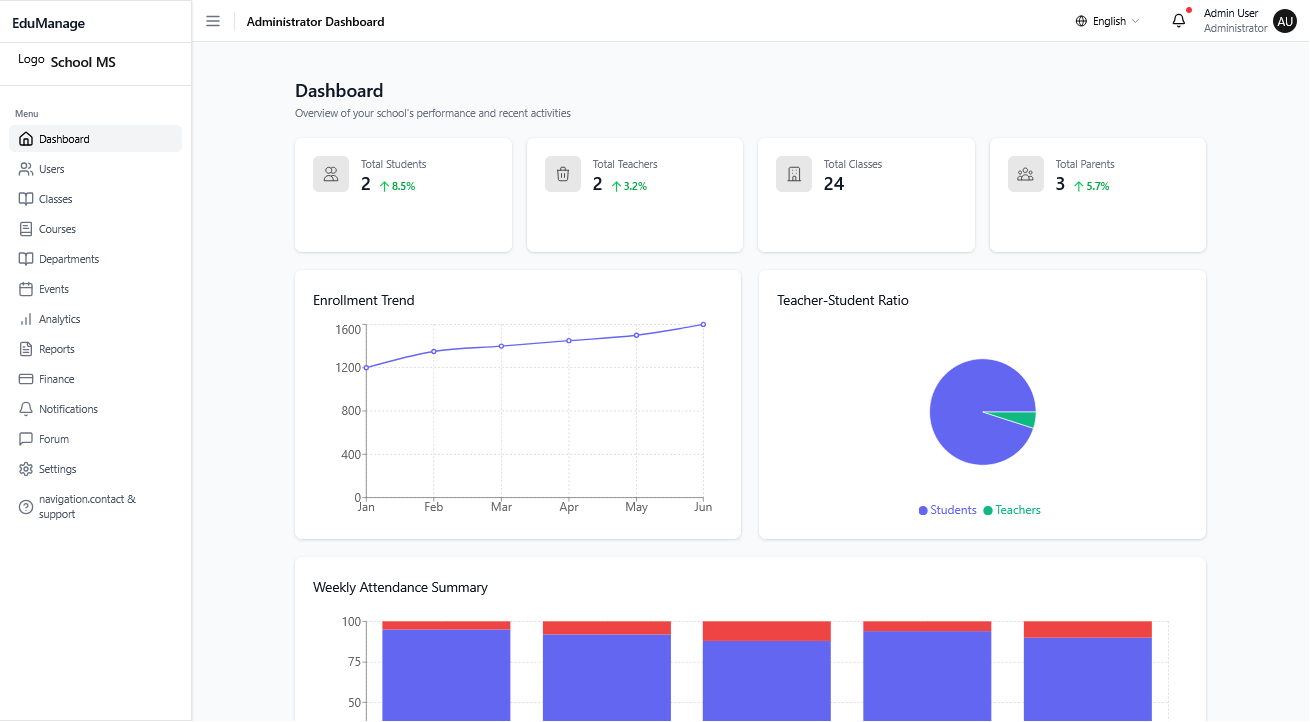
\includegraphics[width=0.85\textwidth,keepaspectratio]{pfe-pics/admin/Screenshot 2025-06-09 at 22-38-06 Vite React TS.png}
  \caption{\textbf{Tableau de bord administrateur} présentant une vue d'ensemble des métriques du système.}
  \label{fig:admin_dashboard}
\end{figure}

Les principales fonctionnalités développées pour l'administrateur comprennent :

\begin{itemize}
  \item \textbf{Tableau de bord analytique} : Visualisation des statistiques clés de l'établissement
  
  \item \textbf{Gestion des utilisateurs} : Interface complète pour créer, modifier et gérer les comptes
  
  \item \textbf{Configuration du système} : Paramètres généraux et personnalisation
  
  \item \textbf{Gestion des cours} : Supervision de tous les cours et programmes
\end{itemize}

\begin{figure}[H]
  \centering
  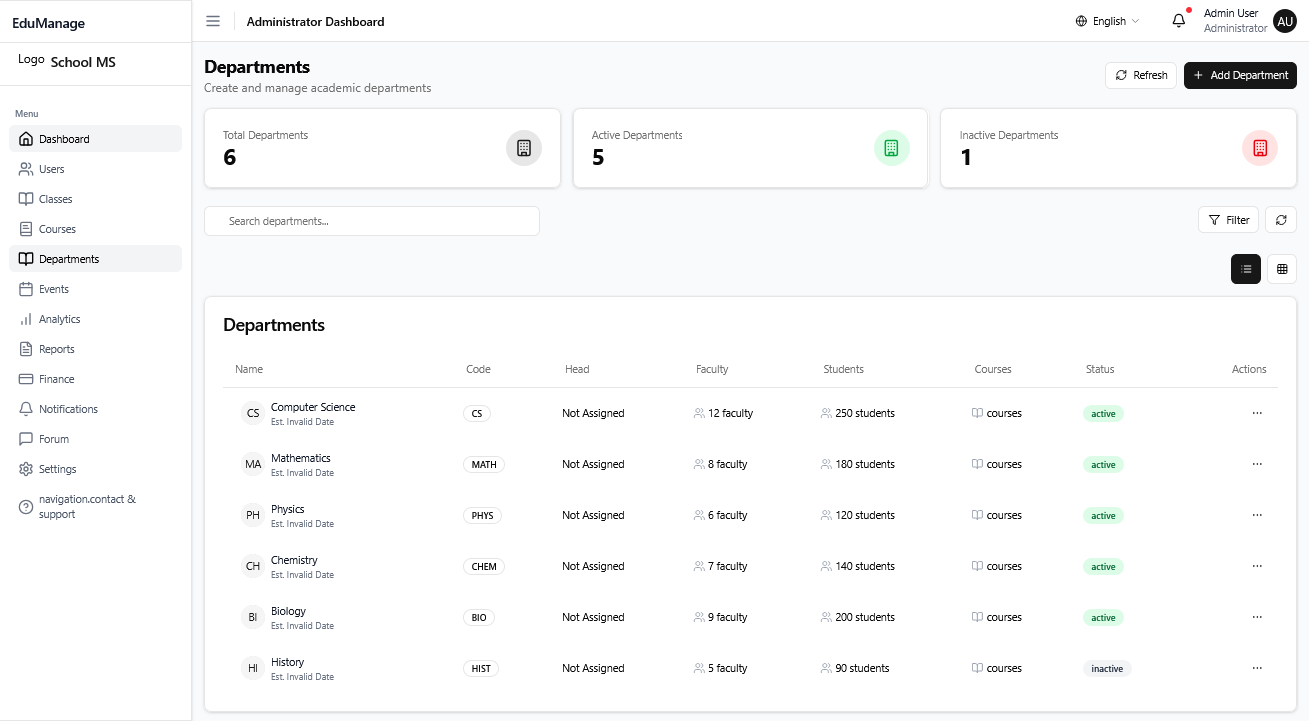
\includegraphics[width=0.85\textwidth,keepaspectratio]{pfe-pics/admin/Screenshot 2025-06-09 at 22-39-15 Vite React TS.png}
  \caption{\textbf{Interface de gestion des utilisateurs} permettant d'administrer les différents types de comptes.}
  \label{fig:user_management}
\end{figure}

\begin{figure}[H]
  \centering
  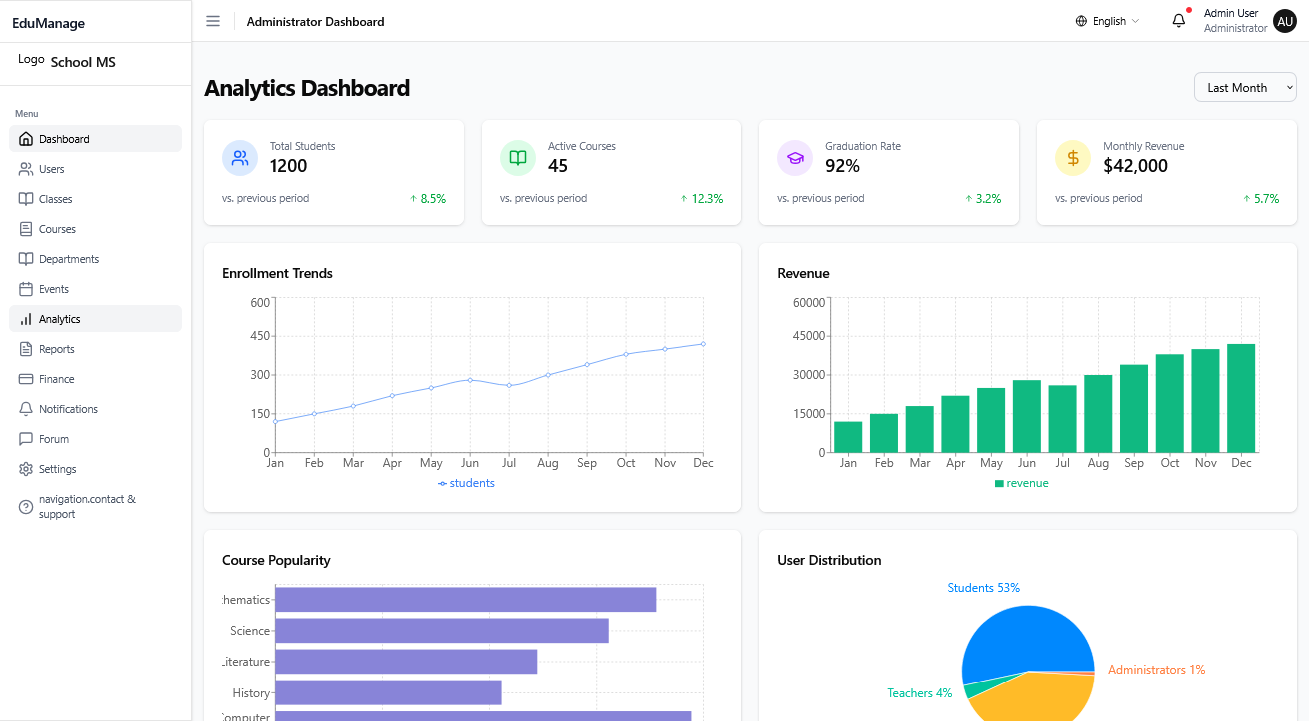
\includegraphics[width=0.85\textwidth,keepaspectratio]{pfe-pics/admin/Screenshot 2025-06-09 at 22-40-11 Vite React TS.png}
  \caption{\textbf{Interface de gestion des cours} avec options de filtrage et d'organisation.}
  \label{fig:course_management_admin}
\end{figure}

\subsubsection{Interface enseignant}

L'interface enseignant a été conçue pour faciliter la gestion pédagogique et le suivi des étudiants :

\begin{figure}[H]
  \centering
  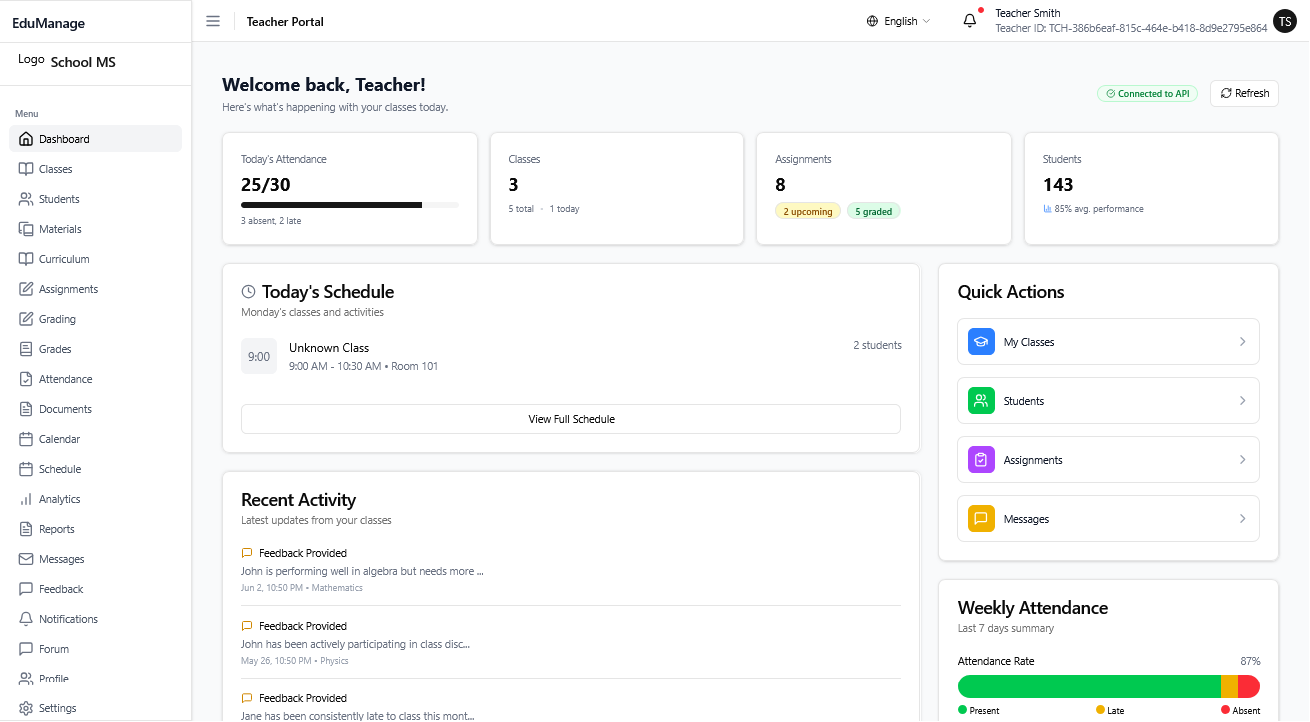
\includegraphics[width=0.85\textwidth,keepaspectratio]{pfe-pics/teacher/Screenshot 2025-06-09 at 22-51-23 Vite React TS.png}
  \caption{\textbf{Tableau de bord enseignant} avec vue d'ensemble des cours et activités récentes.}
  \label{fig:teacher_dashboard}
\end{figure}

Les fonctionnalités clés développées pour les enseignants incluent :

\begin{itemize}
  \item \textbf{Gestion des cours} : Création et organisation du contenu pédagogique
  
  \item \textbf{Suivi des présences} : Interface intuitive pour l'enregistrement des présences
  
  \item \textbf{Évaluation} : Système complet pour la création, notation et commentaire des travaux
  
  \item \textbf{Communication} : Outils pour interagir avec les étudiants et les parents
\end{itemize}

\begin{figure}[H]
  \centering
  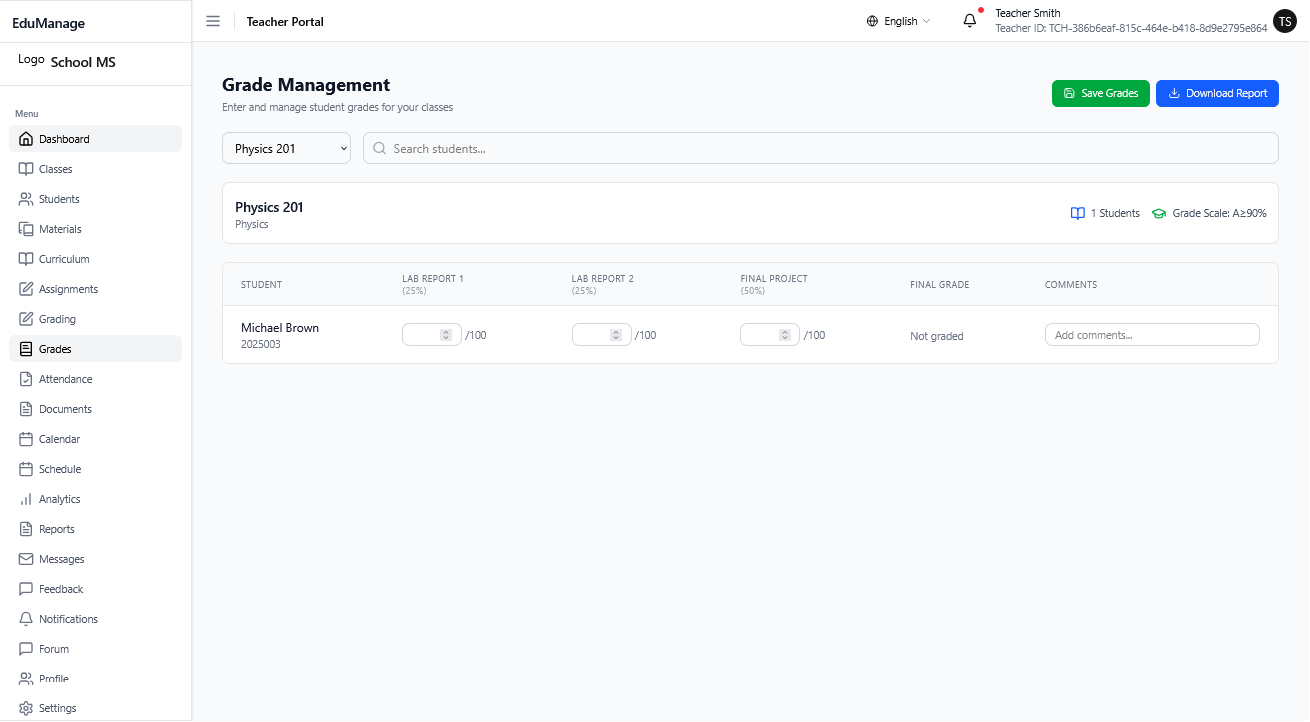
\includegraphics[width=0.85\textwidth,keepaspectratio]{pfe-pics/teacher/Screenshot 2025-06-09 at 22-53-59 Vite React TS.png}
  \caption{\textbf{Interface de prise de présence} permettant un enregistrement rapide et efficace.}
  \label{fig:attendance_taking}
\end{figure}

\begin{figure}[H]
  \centering
  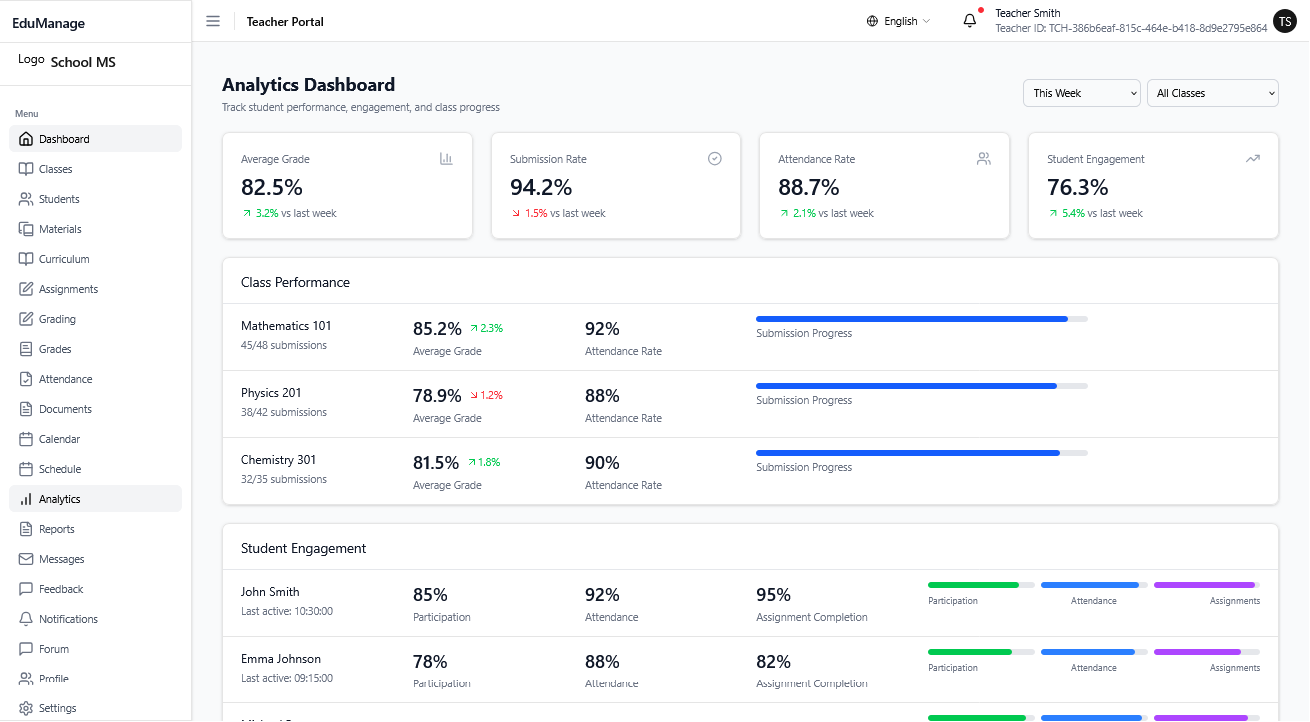
\includegraphics[width=0.85\textwidth,keepaspectratio]{pfe-pics/teacher/Screenshot 2025-06-09 at 22-55-38 Vite React TS.png}
  \caption{\textbf{Interface de notation} avec options de feedback détaillé pour les étudiants.}
  \label{fig:grading_interface}
\end{figure}

\subsubsection{Interface étudiant}

L'interface étudiant a été développée pour offrir un accès clair aux cours, devoirs et résultats :

\begin{figure}[H]
  \centering
  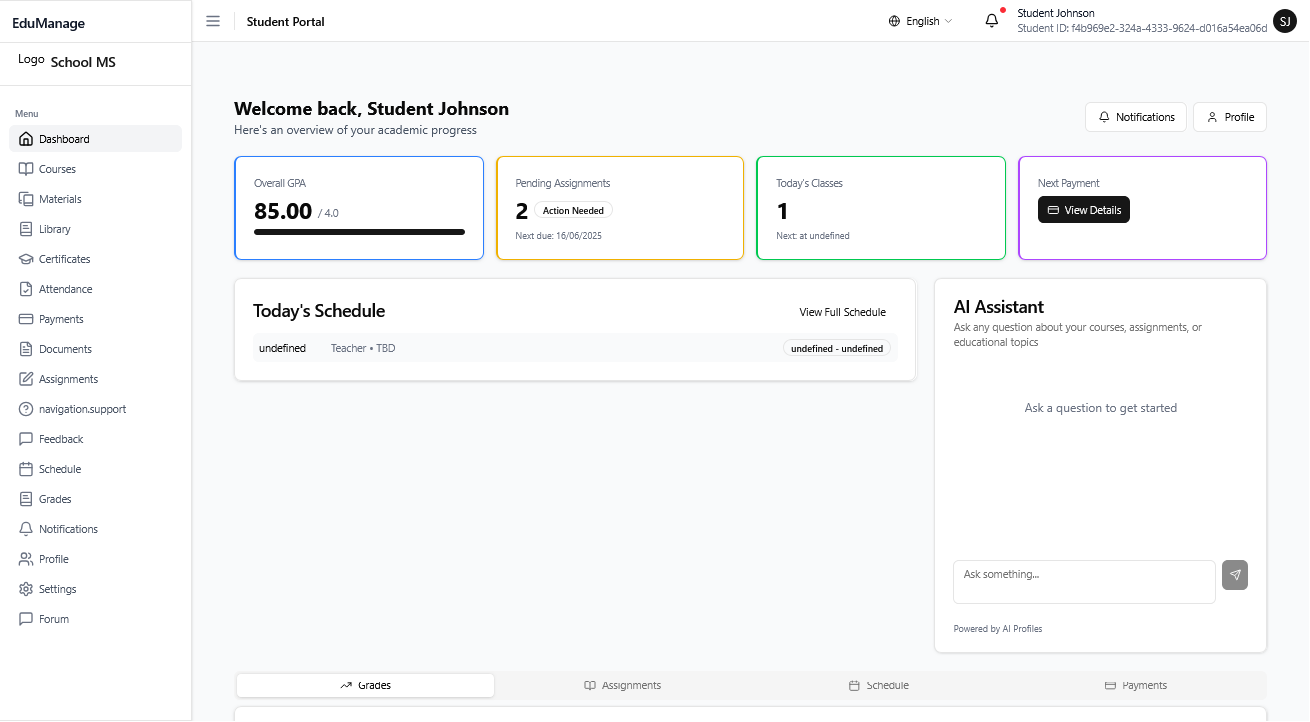
\includegraphics[width=0.85\textwidth,keepaspectratio]{pfe-pics/student/Screenshot 2025-06-09 at 22-43-56 Vite React TS.png}
  \caption{\textbf{Tableau de bord étudiant} présentant les cours, devoirs à venir et notifications.}
  \label{fig:student_dashboard}
\end{figure}

Les principales fonctionnalités pour les étudiants comprennent :

\begin{itemize}
  \item \textbf{Vue d'ensemble des cours} : Accès rapide aux cours suivis et leur contenu
  
  \item \textbf{Calendrier et échéances} : Organisation claire des devoirs et examens à venir
  
  \item \textbf{Soumission de travaux} : Interface intuitive pour déposer les devoirs
  
  \item \textbf{Consultation des résultats} : Visualisation des notes et commentaires des enseignants
\end{itemize}

\begin{figure}[H]
  \centering
  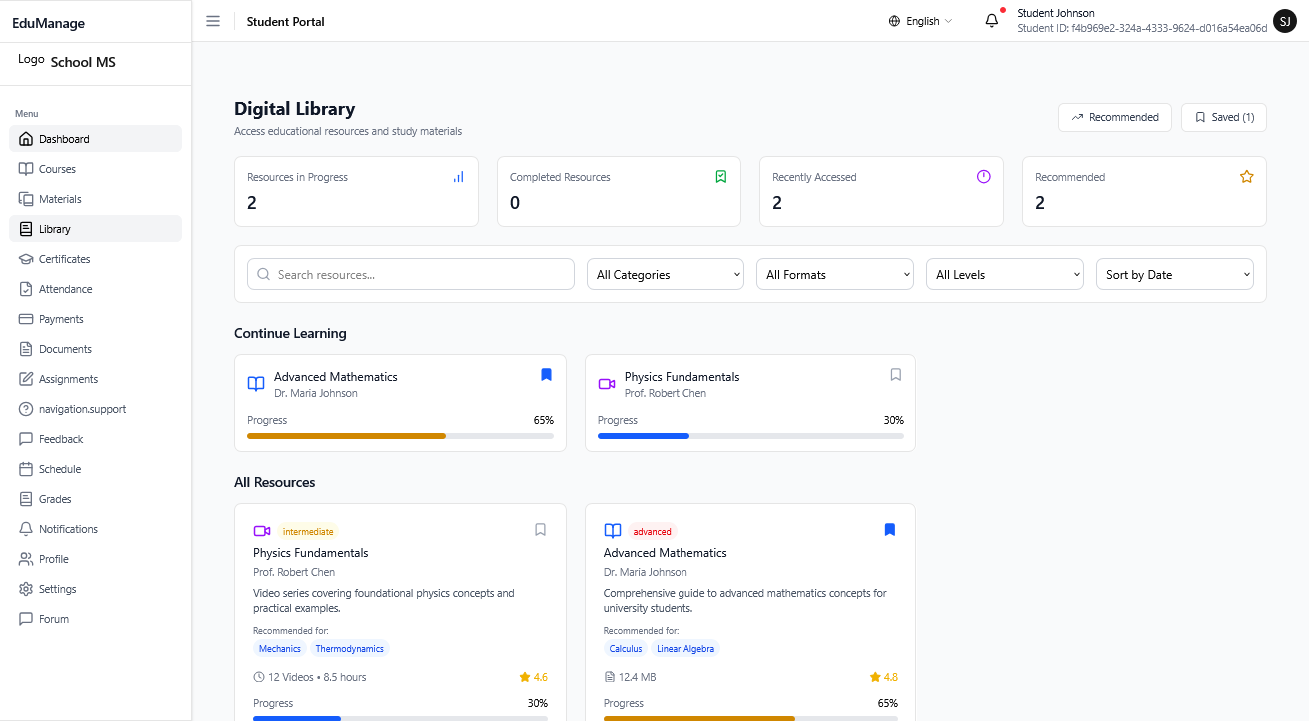
\includegraphics[width=0.85\textwidth,keepaspectratio]{pfe-pics/student/Screenshot 2025-06-09 at 22-45-09 Vite React TS.png}
  \caption{\textbf{Interface de cours} avec accès au matériel pédagogique et aux ressources.}
  \label{fig:course_view}
\end{figure}

\begin{figure}[H]
  \centering
  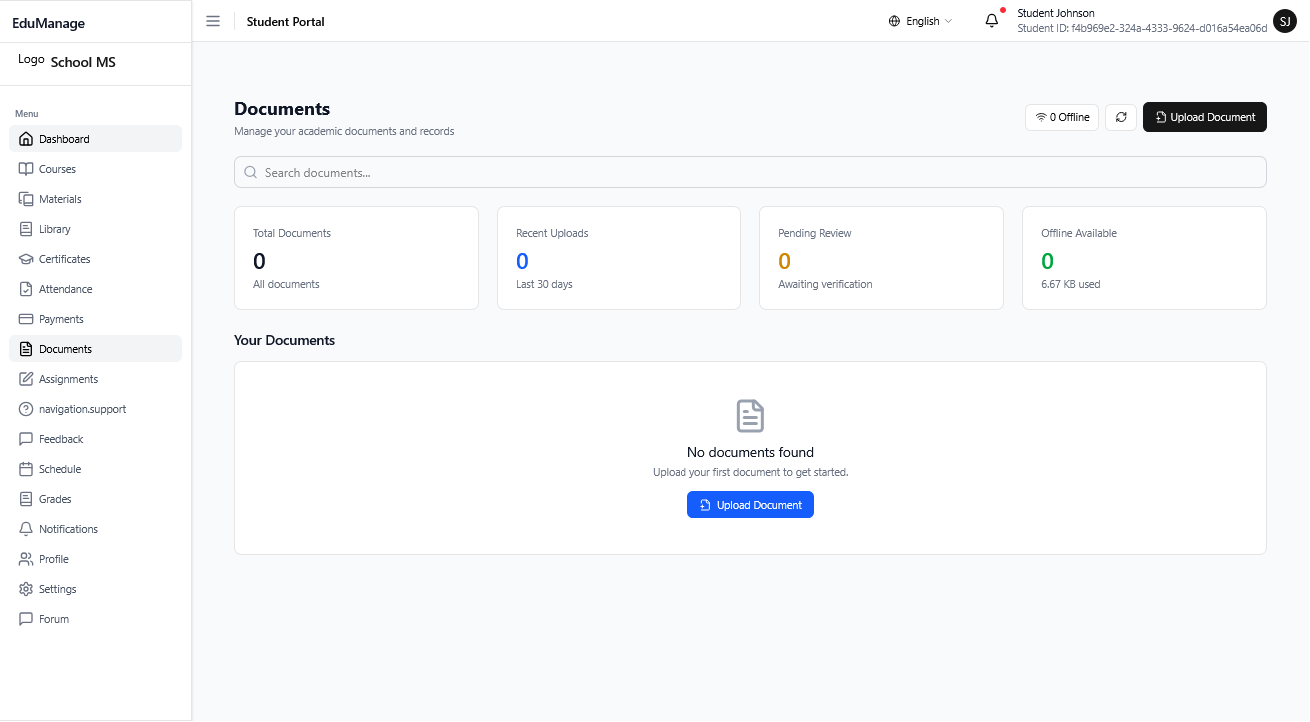
\includegraphics[width=0.85\textwidth,keepaspectratio]{pfe-pics/student/Screenshot 2025-06-09 at 22-46-22 Vite React TS.png}
  \caption{\textbf{Interface de soumission de devoir} avec options d'upload de fichiers.}
  \label{fig:assignment_submission}
\end{figure}

\subsubsection{Interface parent}

L'interface parent permet de suivre efficacement la progression académique des enfants :

\begin{figure}[H]
  \centering
  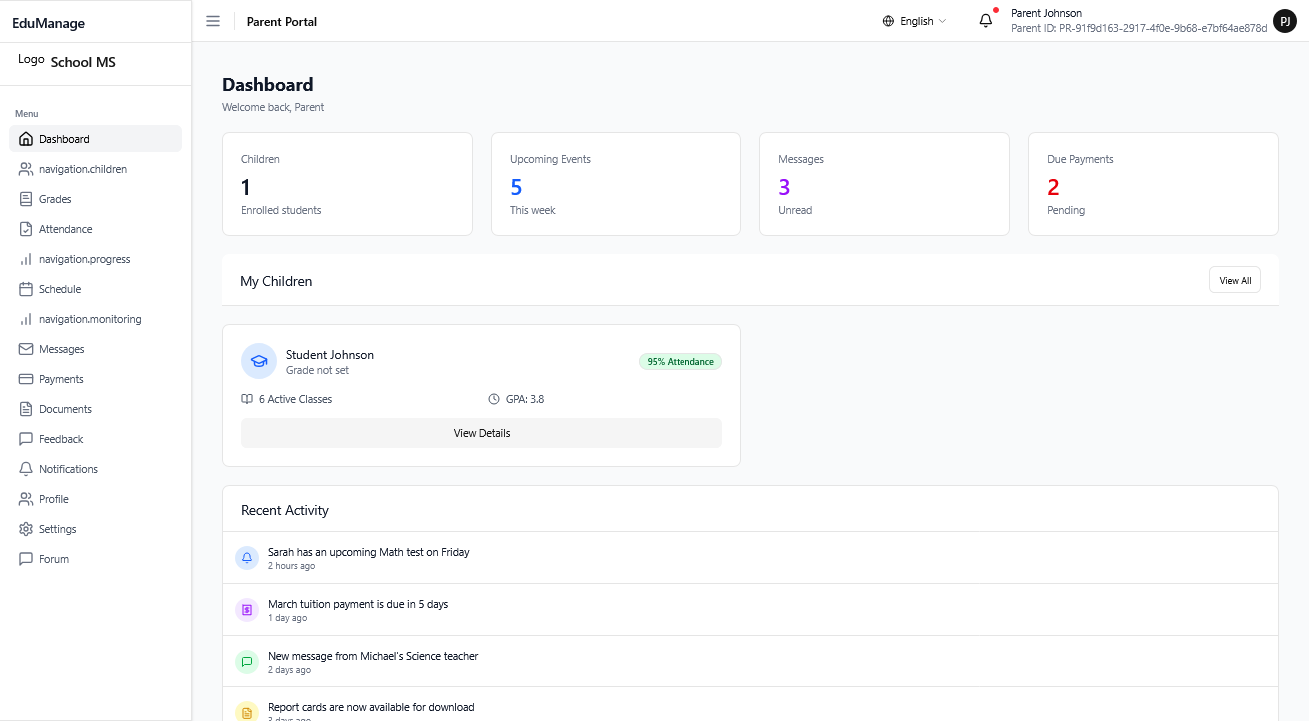
\includegraphics[width=0.85\textwidth,keepaspectratio]{pfe-pics/parent/Screenshot 2025-06-09 at 22-57-22 Vite React TS.png}
  \caption{\textbf{Tableau de bord parent} avec vue d'ensemble des enfants et leurs activités scolaires.}
  \label{fig:parent_dashboard}
\end{figure}

Les fonctionnalités développées pour les parents incluent :

\begin{itemize}
  \item \textbf{Suivi multi-enfants} : Possibilité de suivre plusieurs enfants depuis un seul compte
  
  \item \textbf{Consultation des résultats} : Accès aux notes et évaluations
  
  \item \textbf{Suivi des présences} : Visualisation de l'assiduité de l'enfant
  
  \item \textbf{Communication} : Messagerie directe avec les enseignants et l'administration
\end{itemize}

\begin{figure}[H]
  \centering
  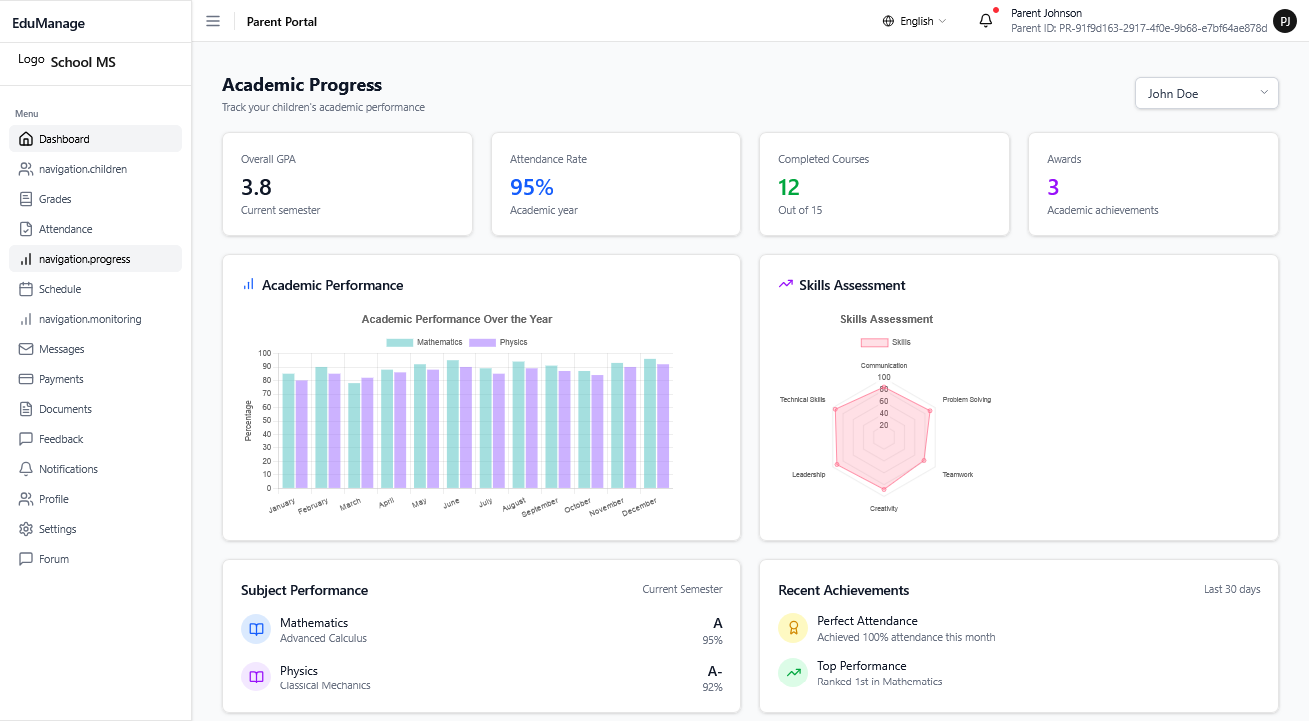
\includegraphics[width=0.85\textwidth,keepaspectratio]{pfe-pics/parent/Screenshot 2025-06-09 at 22-58-13 Vite React TS.png}
  \caption{\textbf{Interface de suivi des résultats} permettant aux parents de visualiser les performances académiques.}
  \label{fig:grades_view}
\end{figure}

\begin{figure}[H]
  \centering
  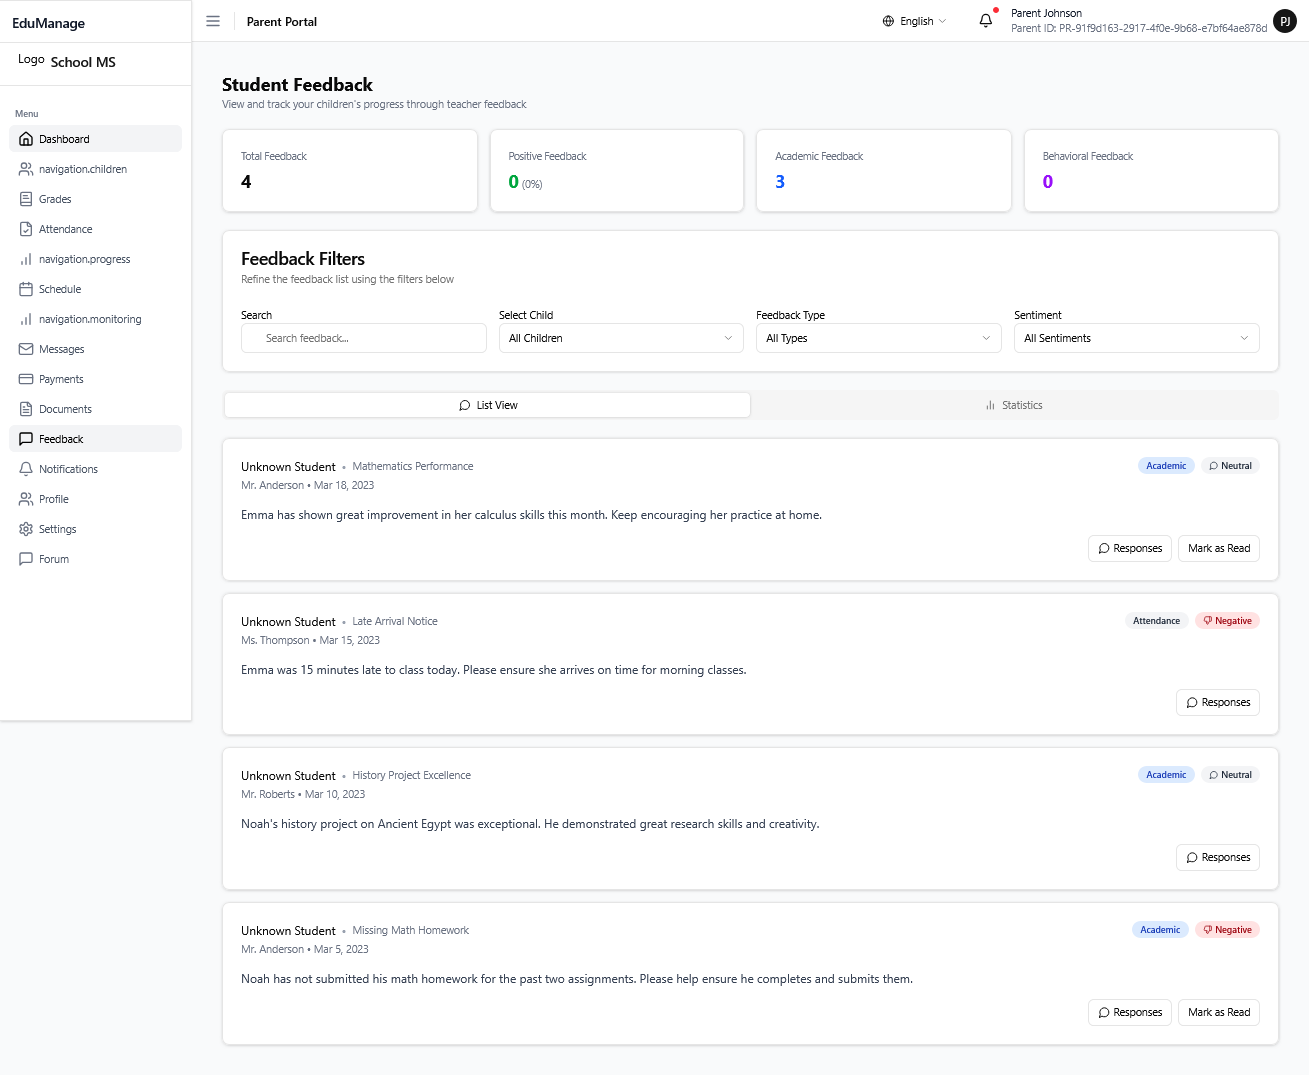
\includegraphics[width=0.85\textwidth,keepaspectratio]{pfe-pics/parent/Screenshot 2025-06-09 at 22-59-25 Vite React TS.png}
  \caption{\textbf{Interface de messagerie} pour la communication avec les enseignants.}
  \label{fig:messaging_interface}
\end{figure}

\subsubsection{Système d'authentification}

Un système d'authentification robuste a été implémenté pour sécuriser l'accès à la plateforme :

\begin{figure}[H]
  \centering
  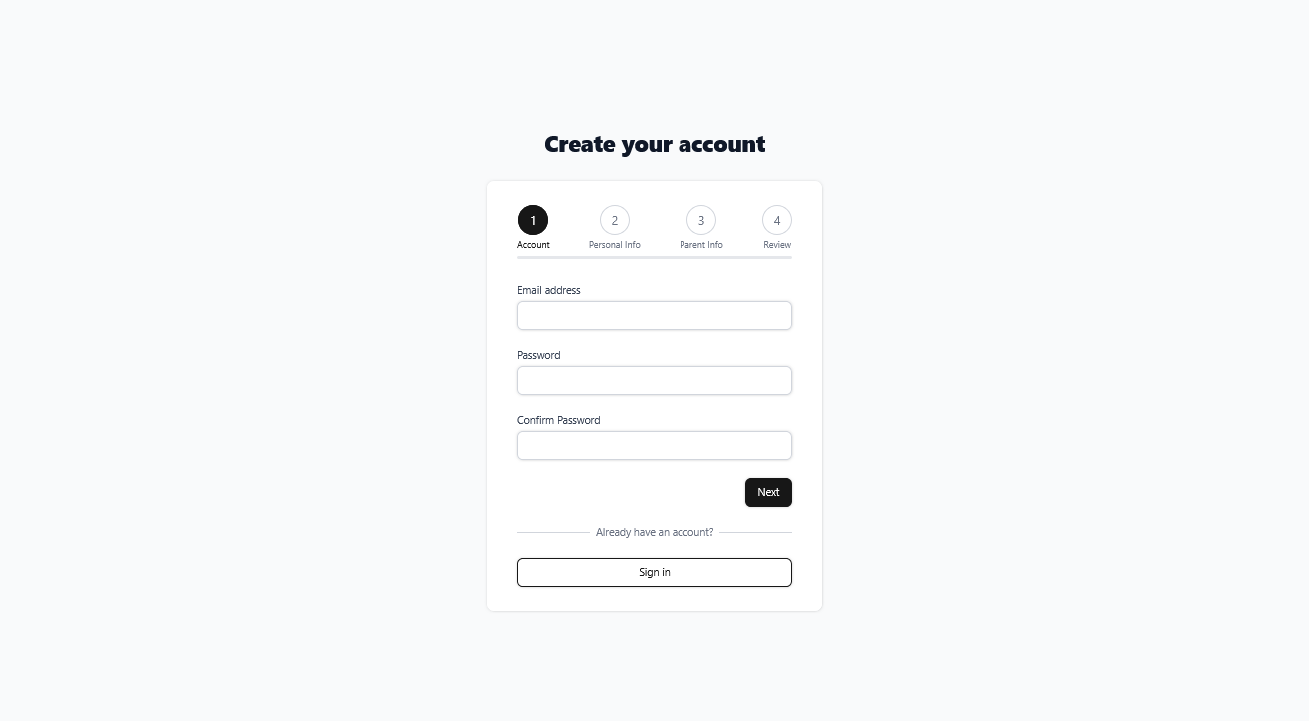
\includegraphics[width=0.6\textwidth,keepaspectratio]{pfe-pics/auth/Screenshot 2025-06-09 at 23-00-18 Vite React TS.png}
  \caption{\textbf{Page de connexion} avec sélection du type d'utilisateur.}
  \label{fig:login_page}
\end{figure}

Les fonctionnalités d'authentification comprennent :

\begin{itemize}
  \item \textbf{Connexion sécurisée} : Authentification avec email et mot de passe
  
  \item \textbf{Récupération de mot de passe} : Procédure sécurisée de réinitialisation
  
  \item \textbf{Vérification d'email} : Confirmation de l'adresse email lors de l'inscription
  
  \item \textbf{Protection des routes} : Accès contrôlé aux différentes sections selon le rôle
\end{itemize}

\begin{figure}[H]
  \centering
  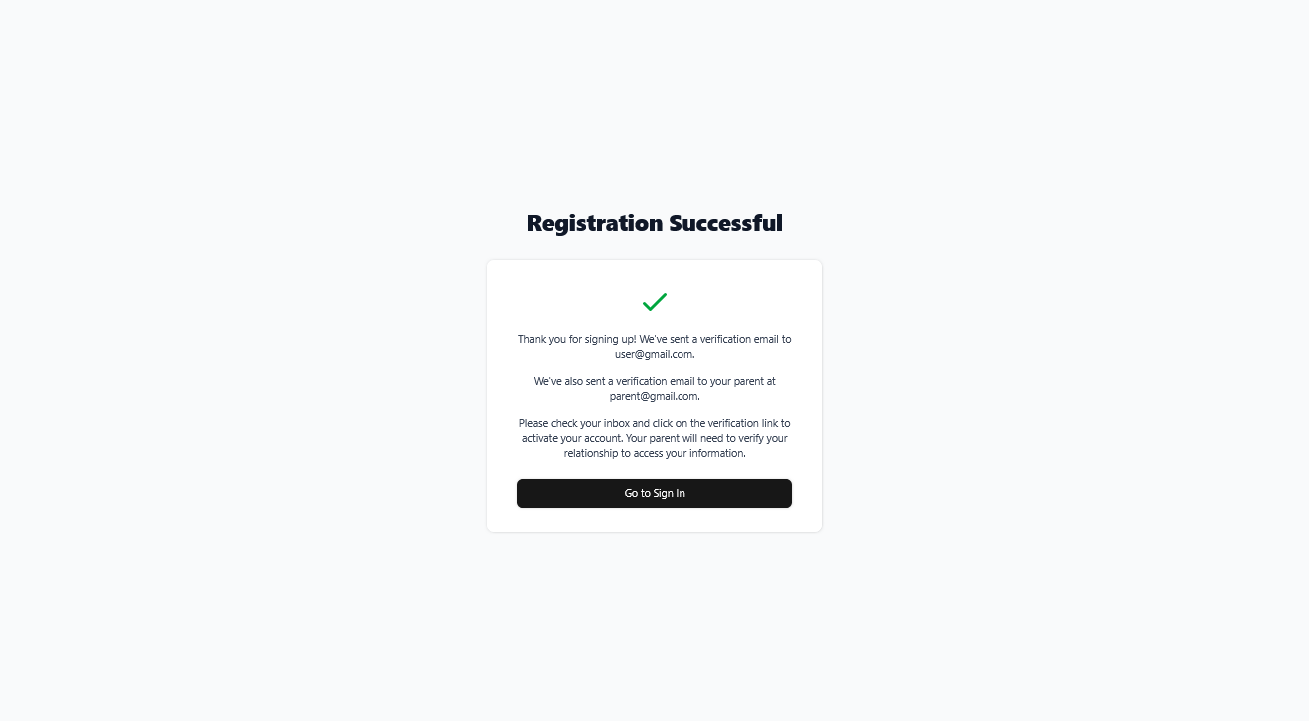
\includegraphics[width=0.6\textwidth,keepaspectratio]{pfe-pics/auth/Screenshot 2025-06-09 at 23-02-10 Vite React TS.png}
  \caption{\textbf{Interface de récupération de mot de passe} avec vérification par email.}
  \label{fig:password_reset}
\end{figure}

\begin{figure}[H]
  \centering
  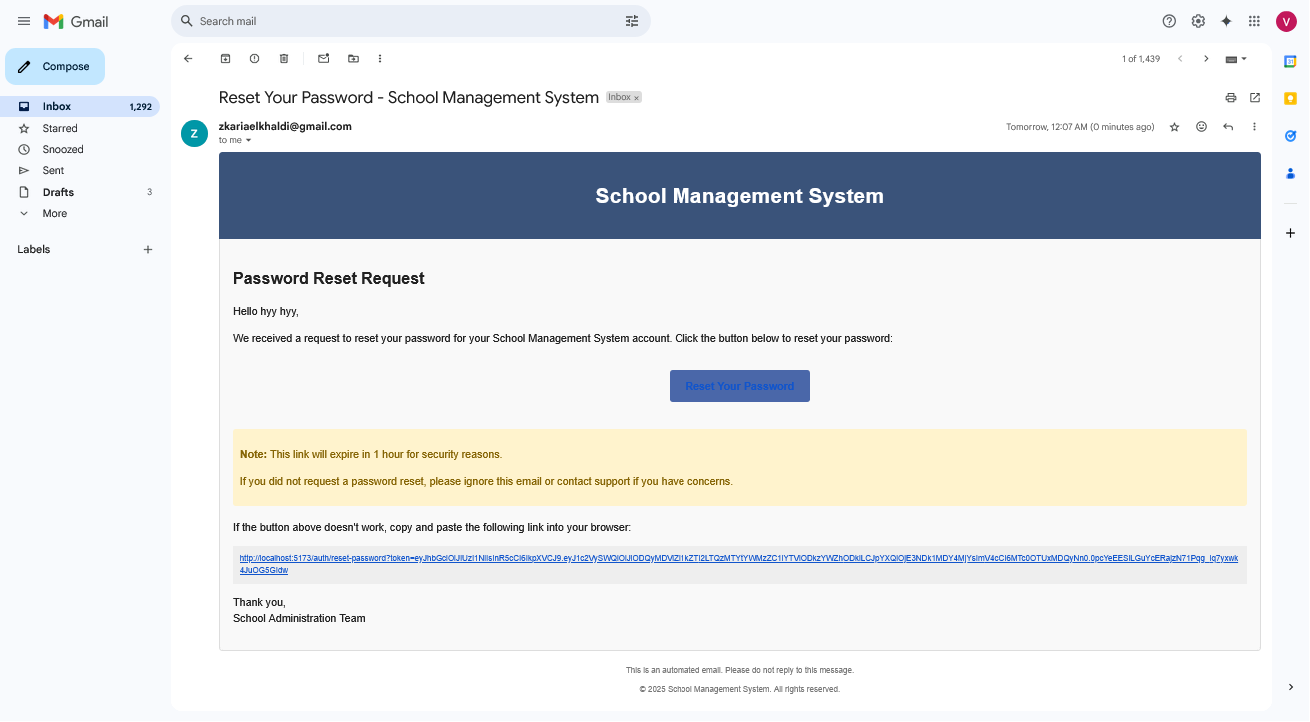
\includegraphics[width=0.85\textwidth,keepaspectratio]{pfe-pics/auth/Screenshot 2025-06-09 at 23-08-41 Reset Your Password - School Management System - vertigoevilman1@gmail.com - Gmail.png}
  \caption{\textbf{Email de réinitialisation de mot de passe} envoyé aux utilisateurs.}
  \label{fig:password_reset_email}
\end{figure}

\subsection{Développement des applications mobiles}

\subsubsection{Architecture de l'application mobile}

L'application mobile a été développée avec React Native et Expo pour offrir une expérience utilisateur native sur iOS et Android tout en partageant une base de code commune. L'architecture adoptée suit le modèle de composants React avec une gestion d'état centralisée.

\begin{itemize}
  \item \textbf{Structure du projet} : Organisation en modules fonctionnels avec séparation des préoccupations
  
  \item \textbf{Navigation} : Utilisation de React Navigation pour une expérience de navigation fluide
  
  \item \textbf{Gestion d'état} : Combinaison de Context API et de React Query pour la gestion des données
  
  \item \textbf{Composants réutilisables} : Bibliothèque de composants partagés entre les différentes vues
  
  \item \textbf{Adaptation responsive} : Interfaces s'adaptant aux différentes tailles d'écran
\end{itemize}

\subsubsection{Interfaces mobiles pour les étudiants}

L'application mobile offre aux étudiants un accès optimisé à leurs cours et activités :

\begin{figure}[H]
  \centering
  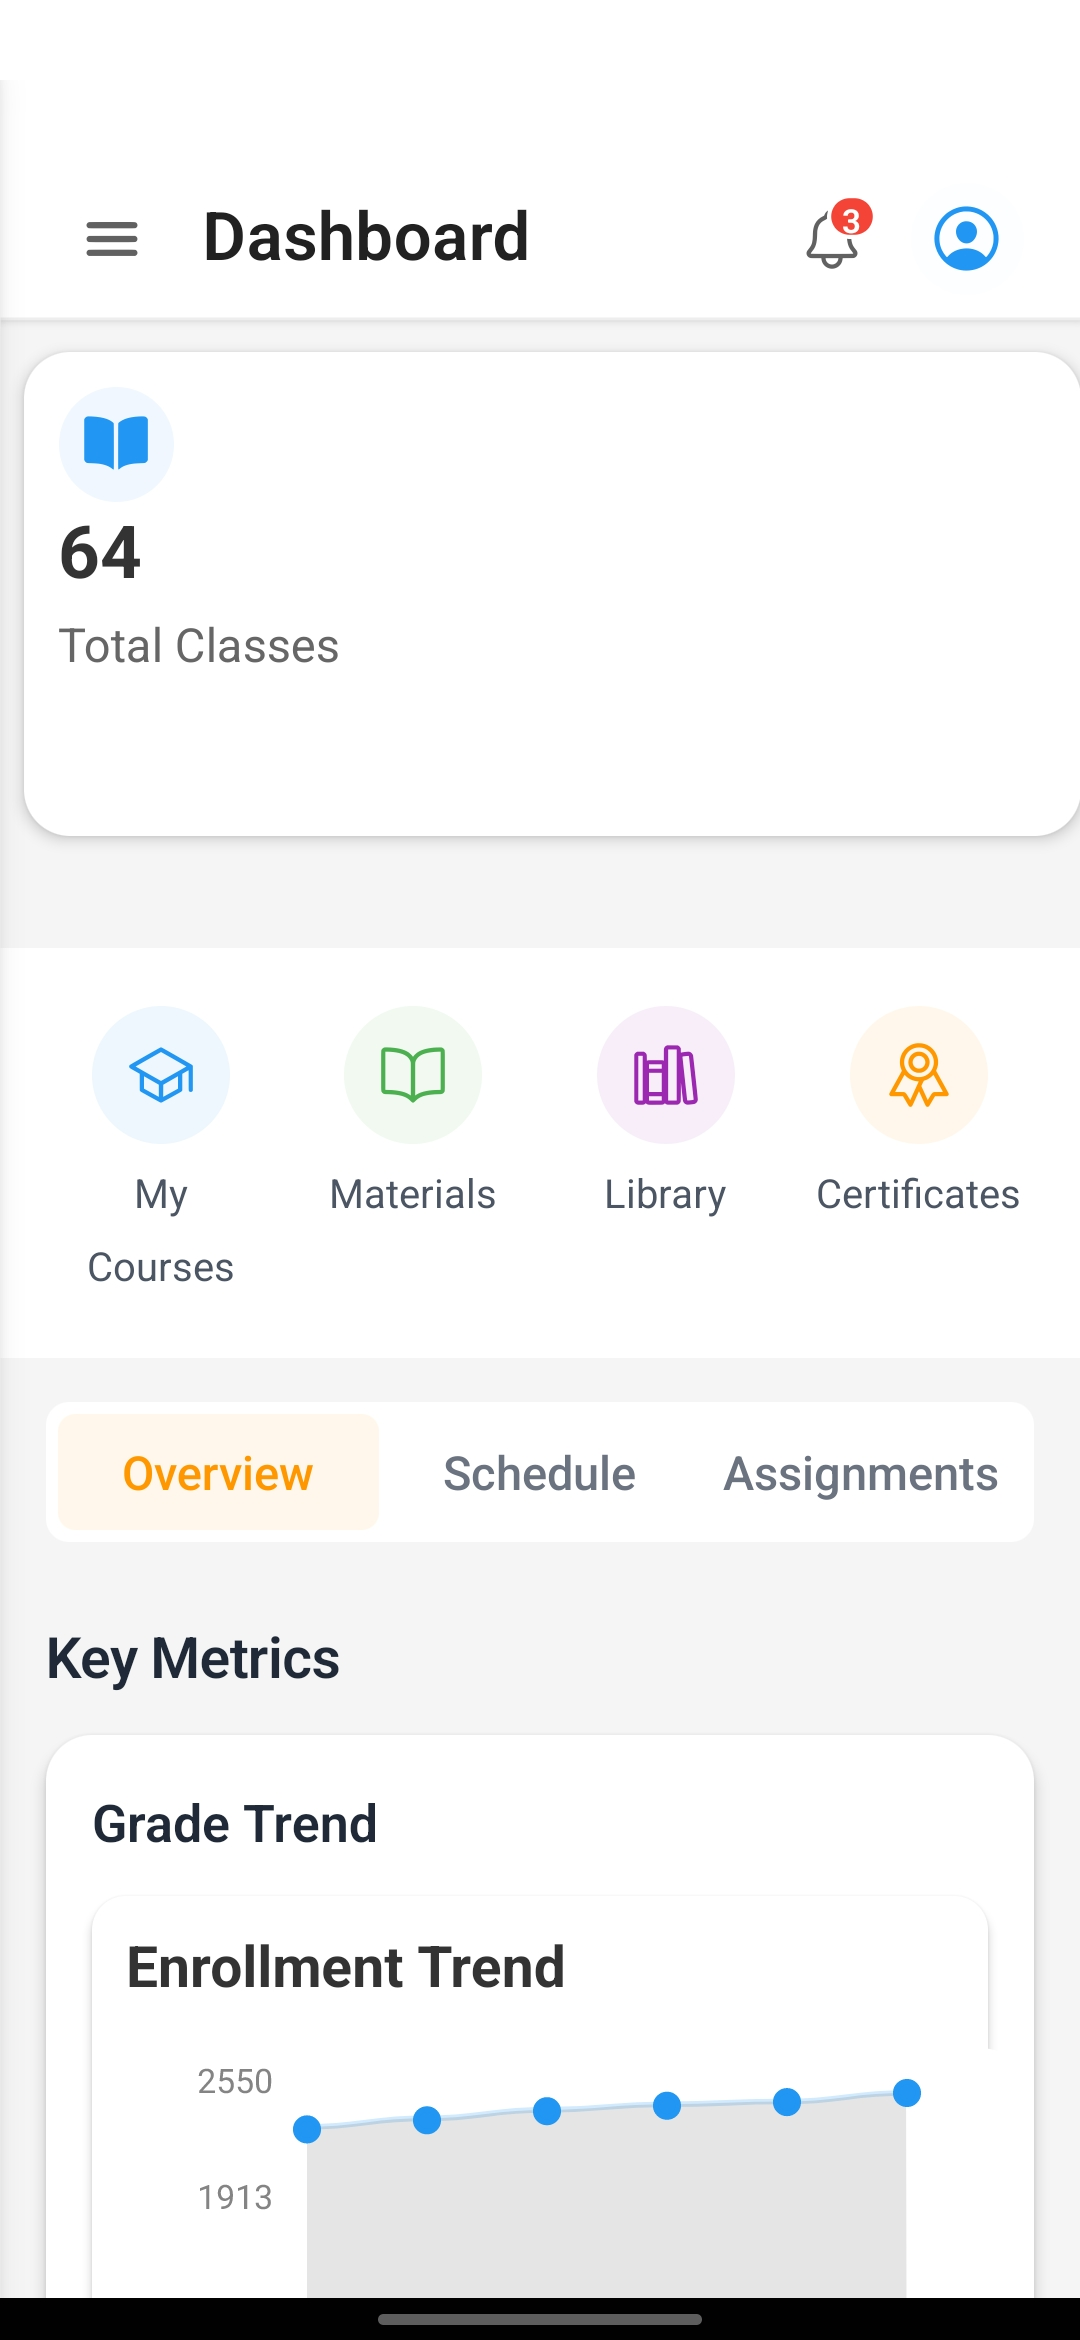
\includegraphics[width=0.4\textwidth,keepaspectratio]{pfe-pics/Mobile /Students/Screenshot_20250610_130022_Expo Go.jpg}
  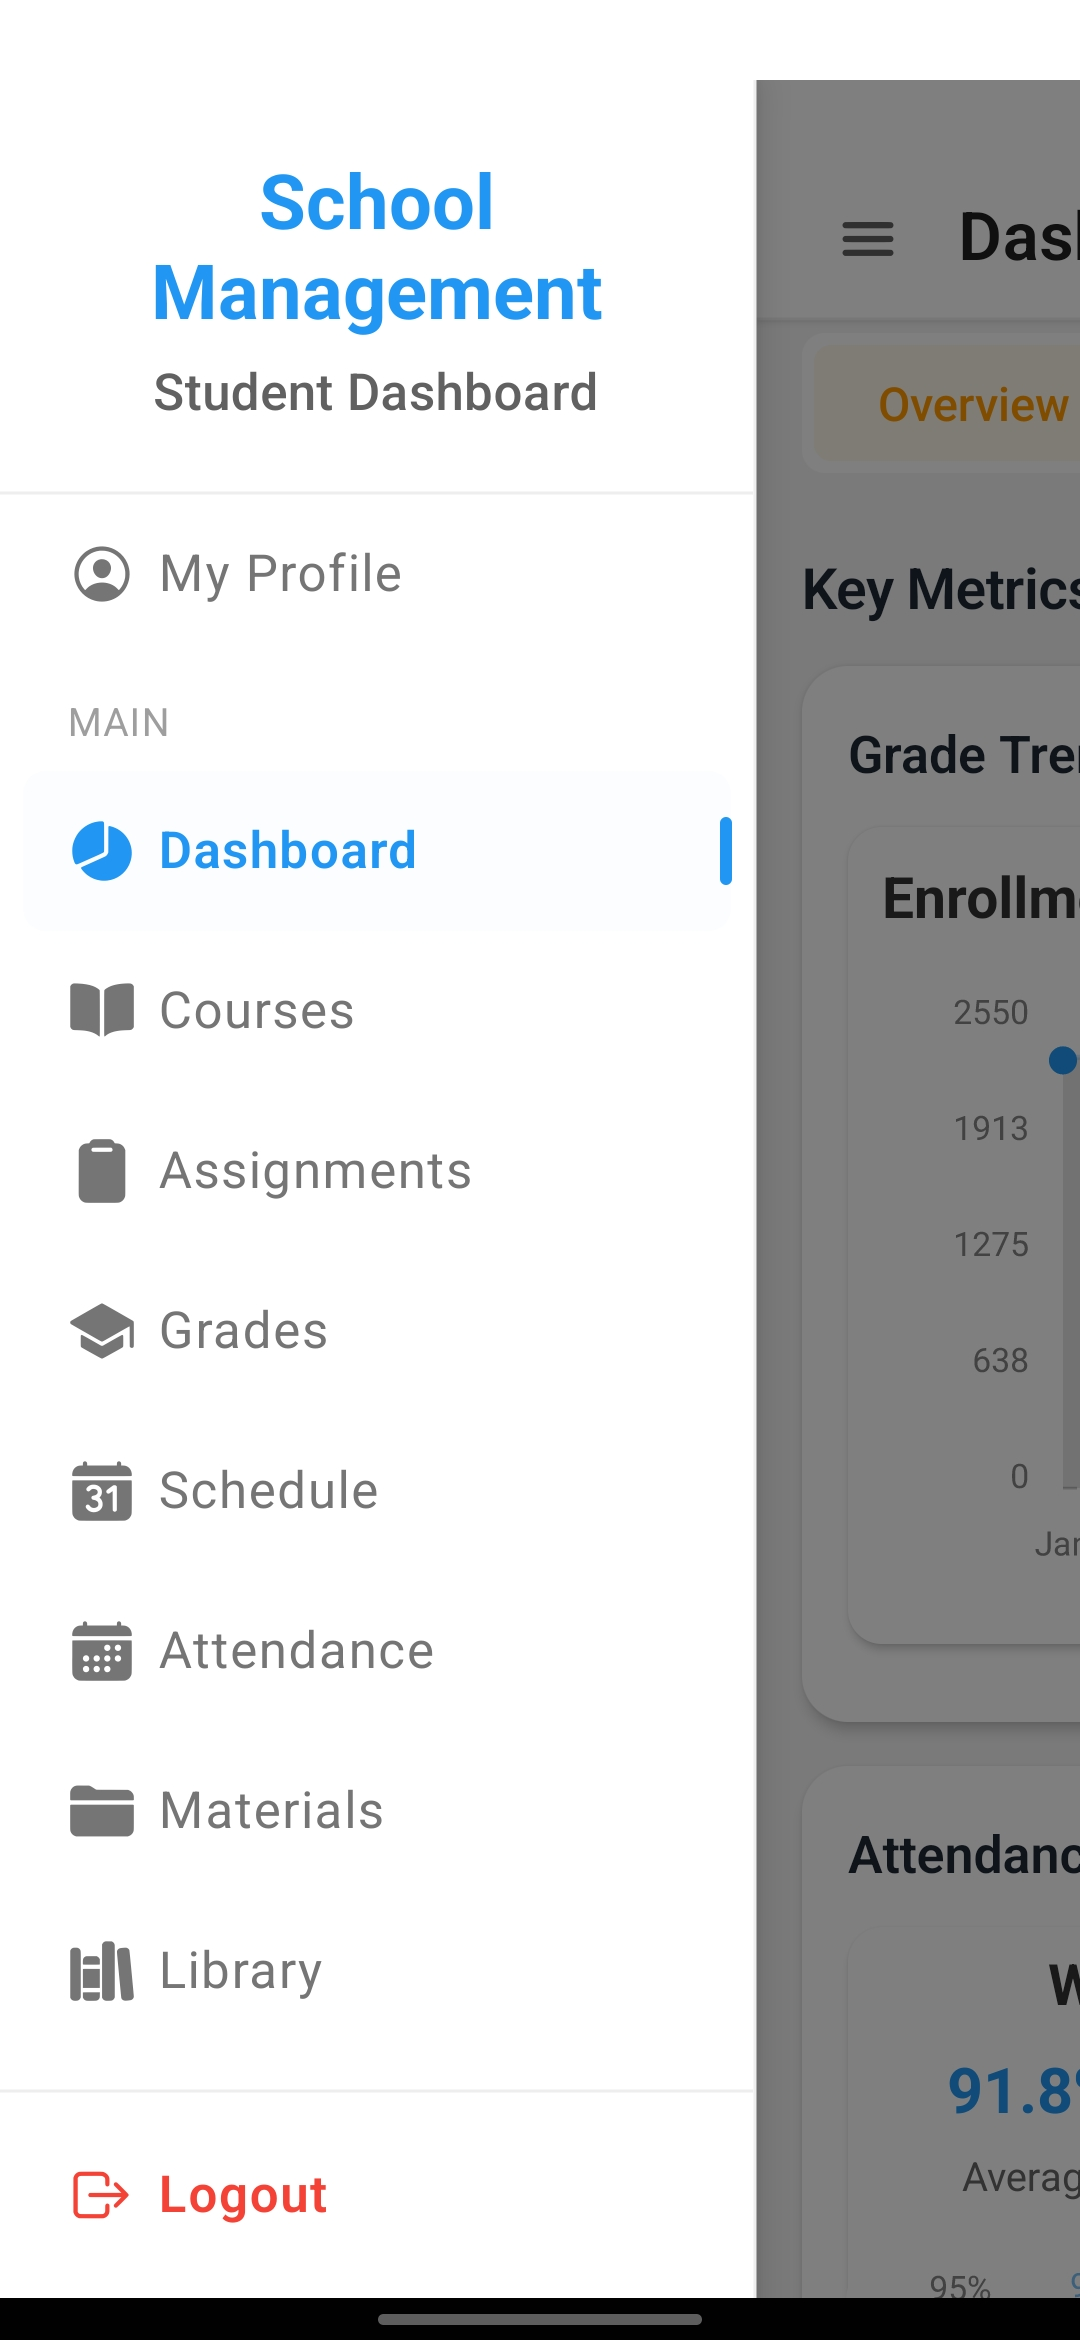
\includegraphics[width=0.4\textwidth,keepaspectratio]{pfe-pics/Mobile /Students/Screenshot_20250610_130124_Expo Go.jpg}
  \caption{\textbf{Écrans d'accueil et de cours} de l'application mobile pour les étudiants.}
  \label{fig:mobile_student_home}
\end{figure}

\begin{figure}[H]
  \centering
  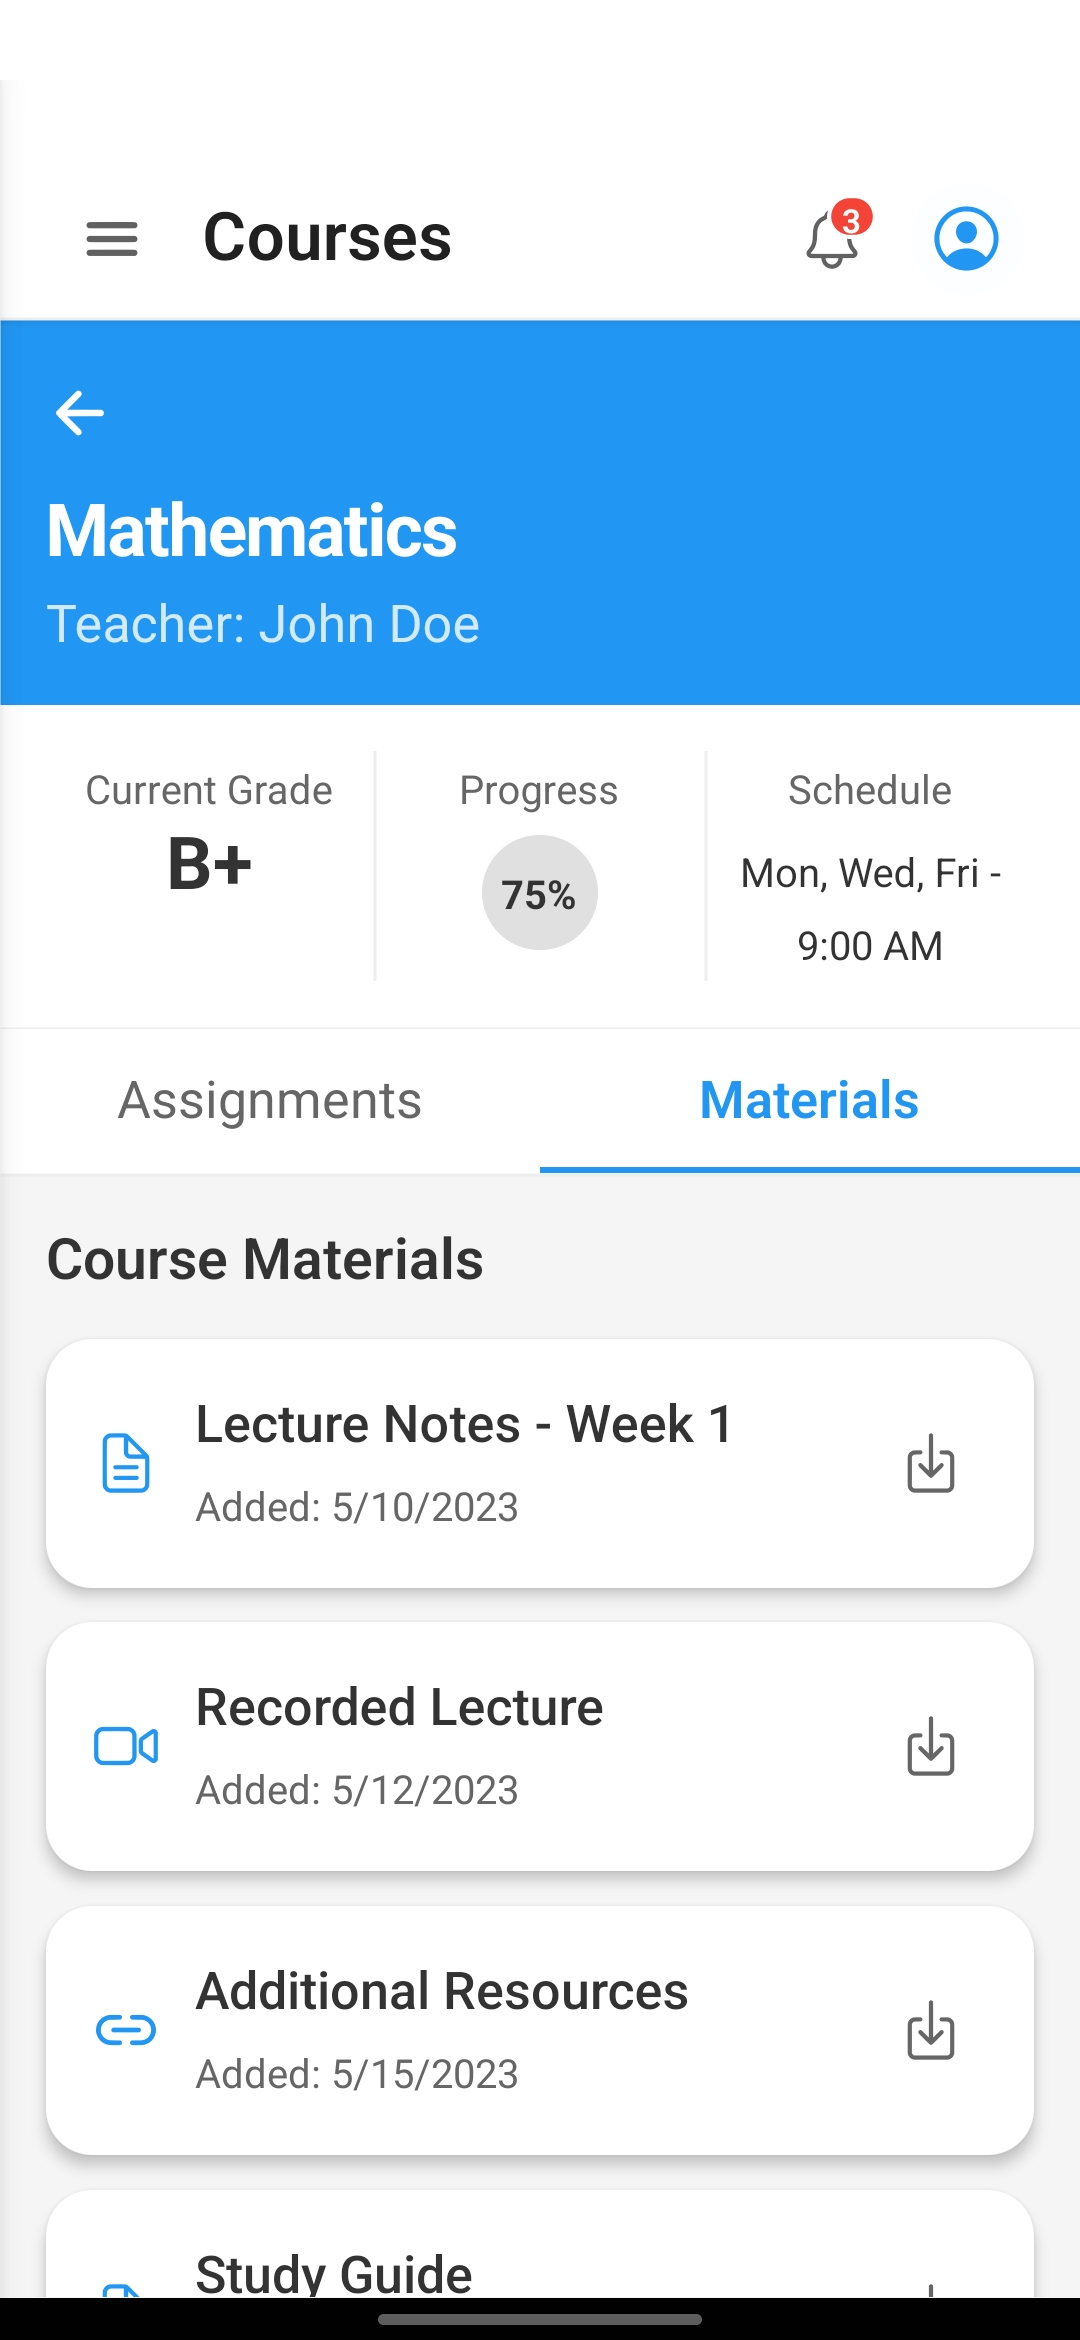
\includegraphics[width=0.4\textwidth,keepaspectratio]{pfe-pics/Mobile /Students/Screenshot_20250610_130150_Expo Go.jpg}
  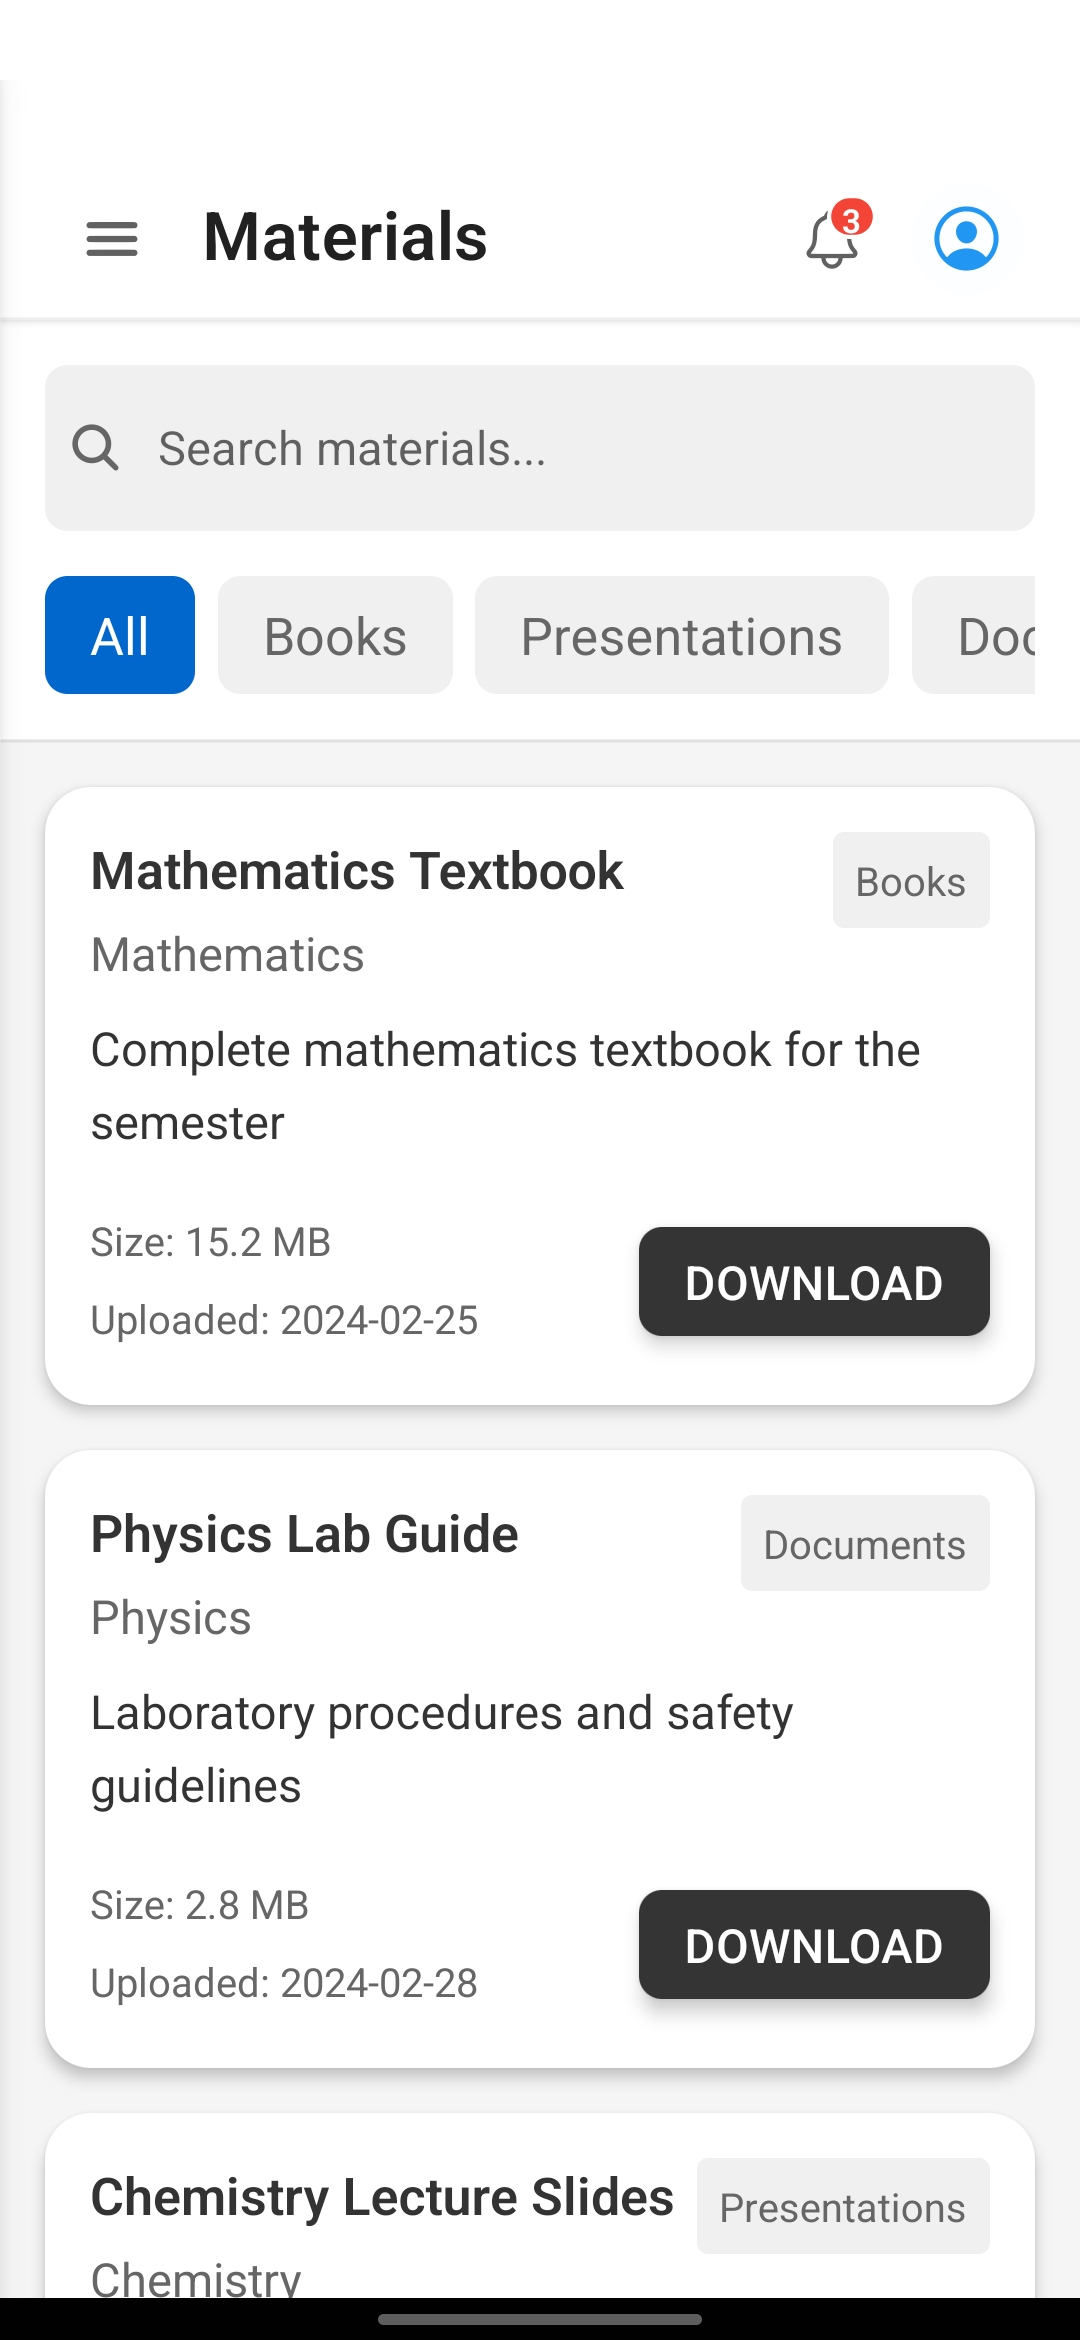
\includegraphics[width=0.4\textwidth,keepaspectratio]{pfe-pics/Mobile /Students/Screenshot_20250610_130310_Expo Go.jpg}
  \caption{\textbf{Interfaces de consultation des devoirs et résultats} sur mobile.}
  \label{fig:mobile_student_assignments}
\end{figure}

\subsubsection{Interfaces mobiles pour les enseignants}

Les enseignants bénéficient d'une application mobile adaptée à leurs besoins spécifiques :

\begin{figure}[H]
  \centering
  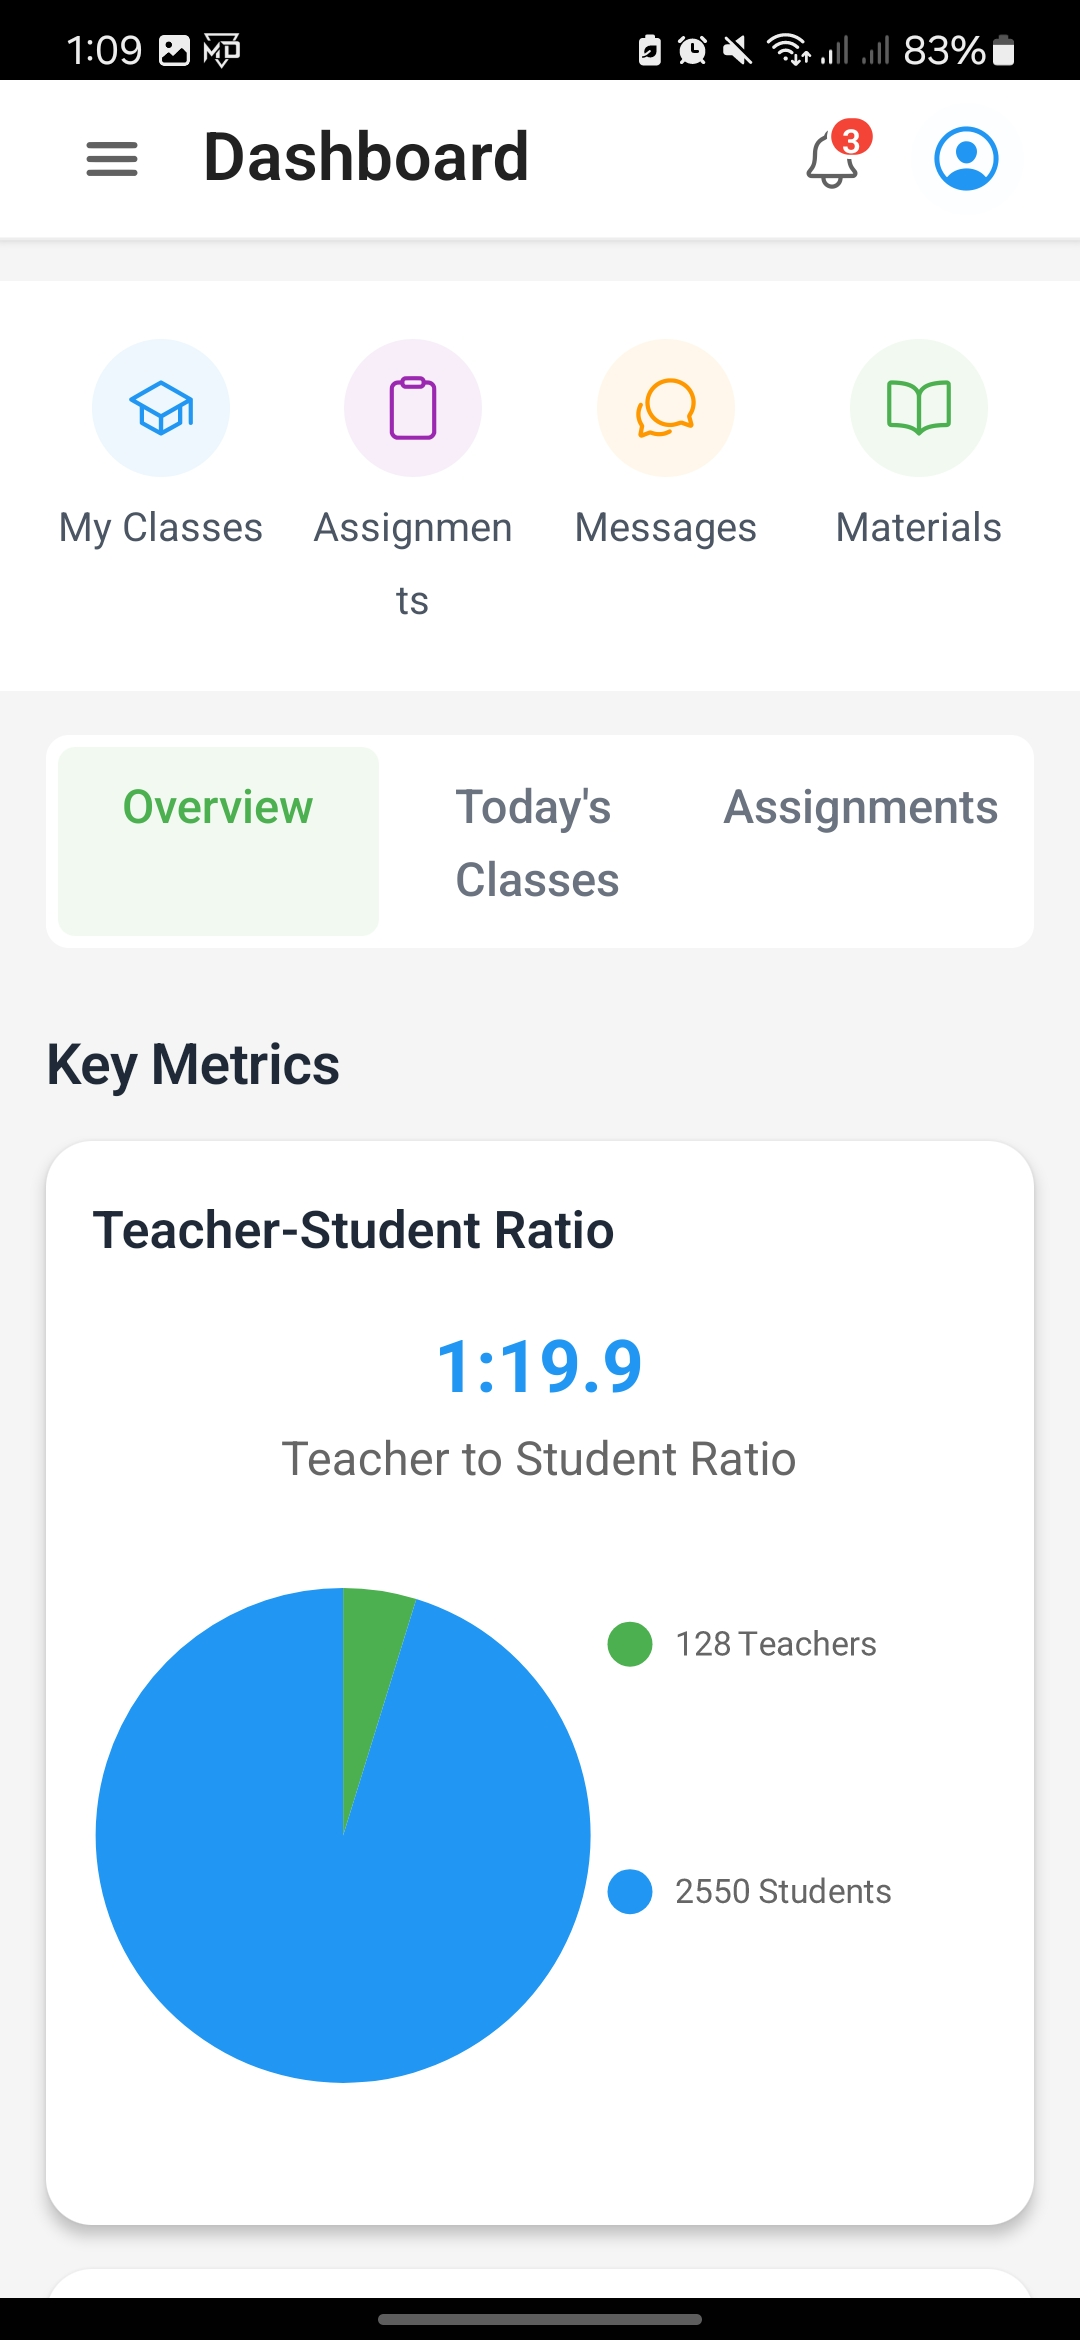
\includegraphics[width=0.4\textwidth,keepaspectratio]{pfe-pics/Mobile /Teacher/Screenshot_20250610_130952_Expo Go.jpg}
  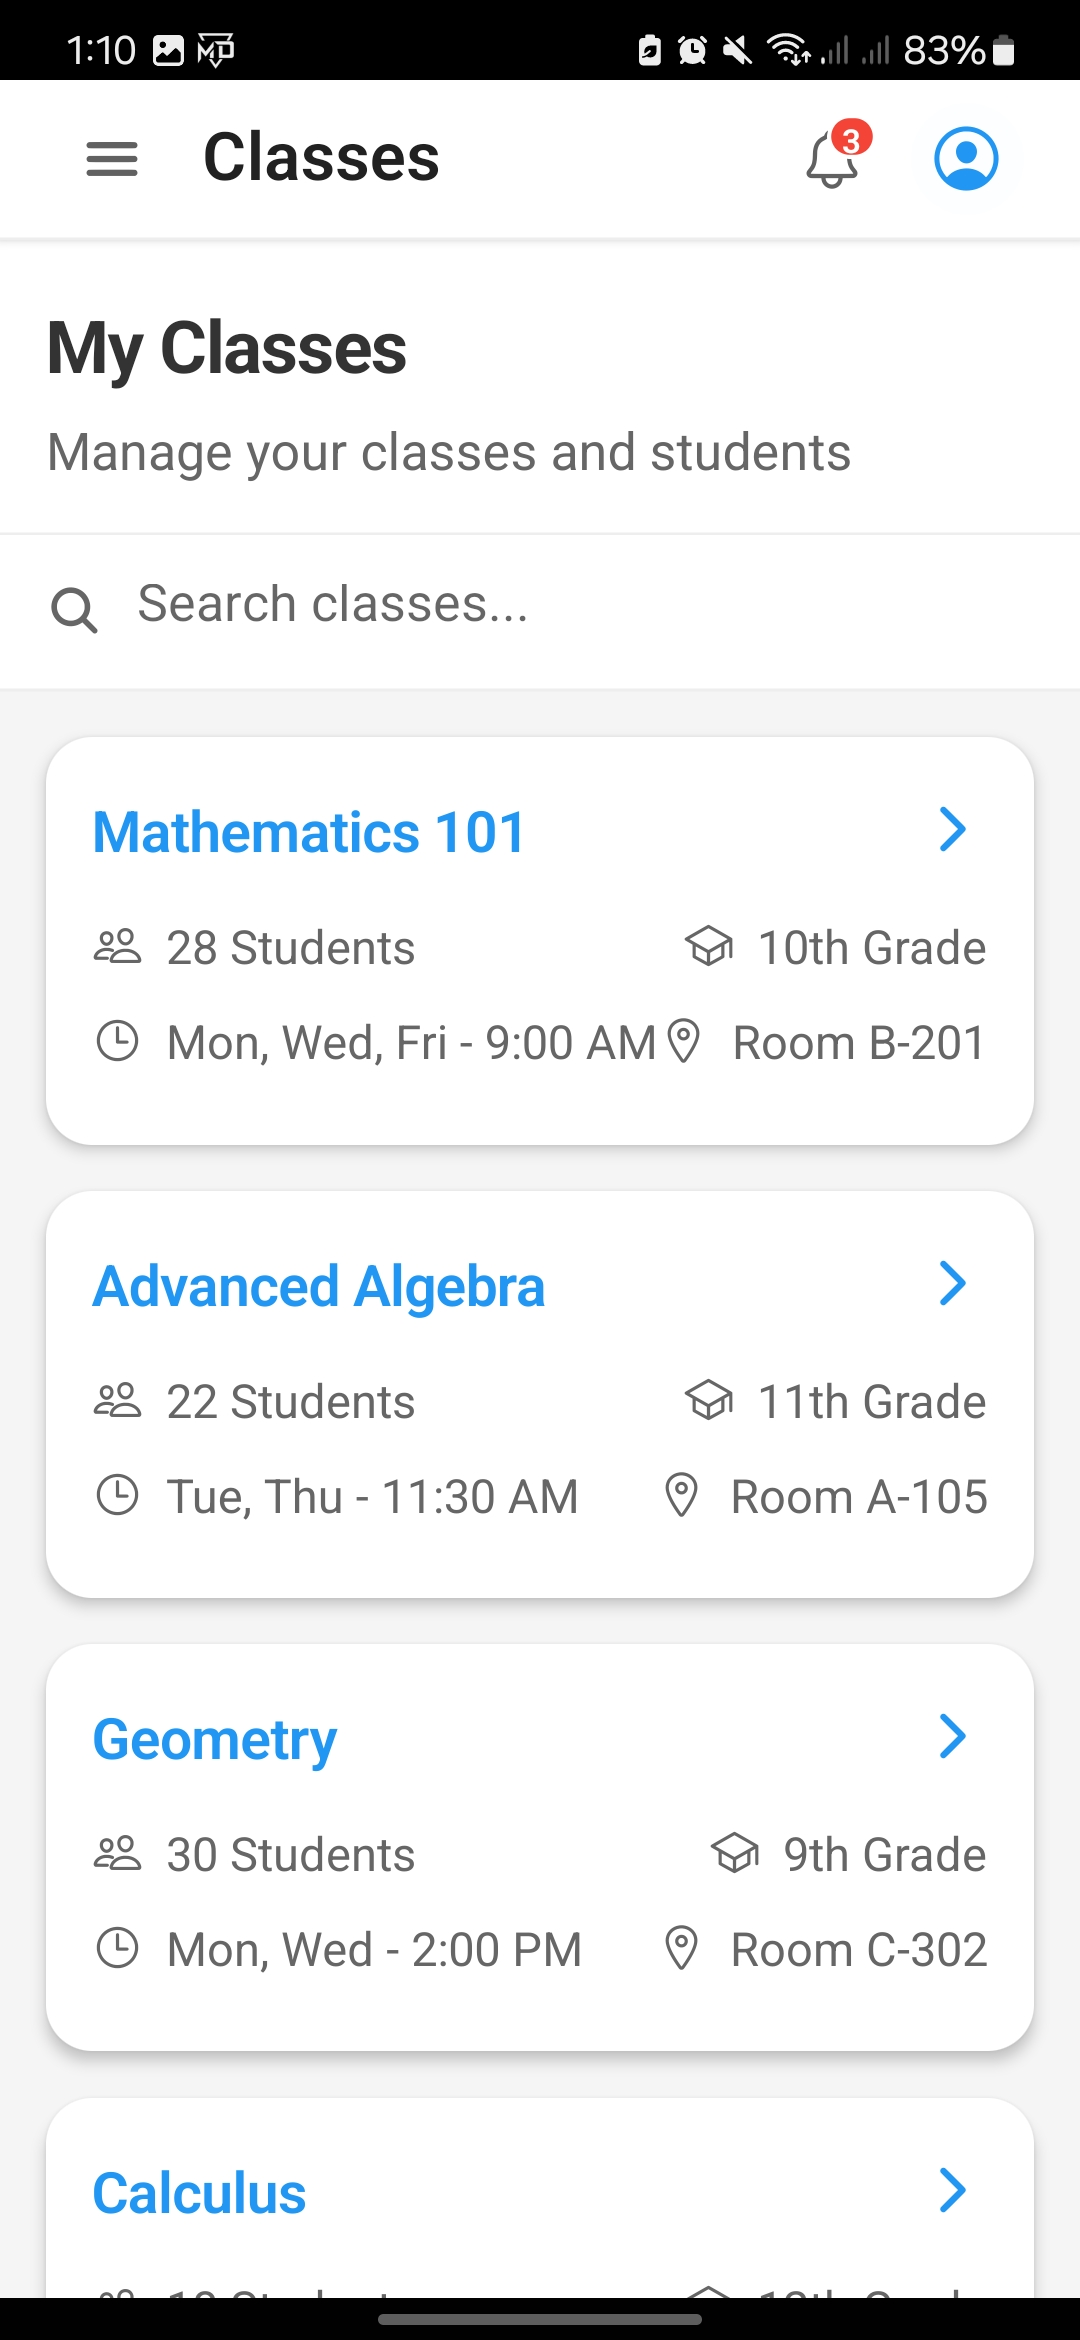
\includegraphics[width=0.4\textwidth,keepaspectratio]{pfe-pics/Mobile /Teacher/Screenshot_20250610_131009_Expo Go.jpg}
  \caption{\textbf{Tableau de bord et liste des cours} sur l'application mobile enseignant.}
  \label{fig:mobile_teacher_dashboard}
\end{figure}

\begin{figure}[H]
  \centering
  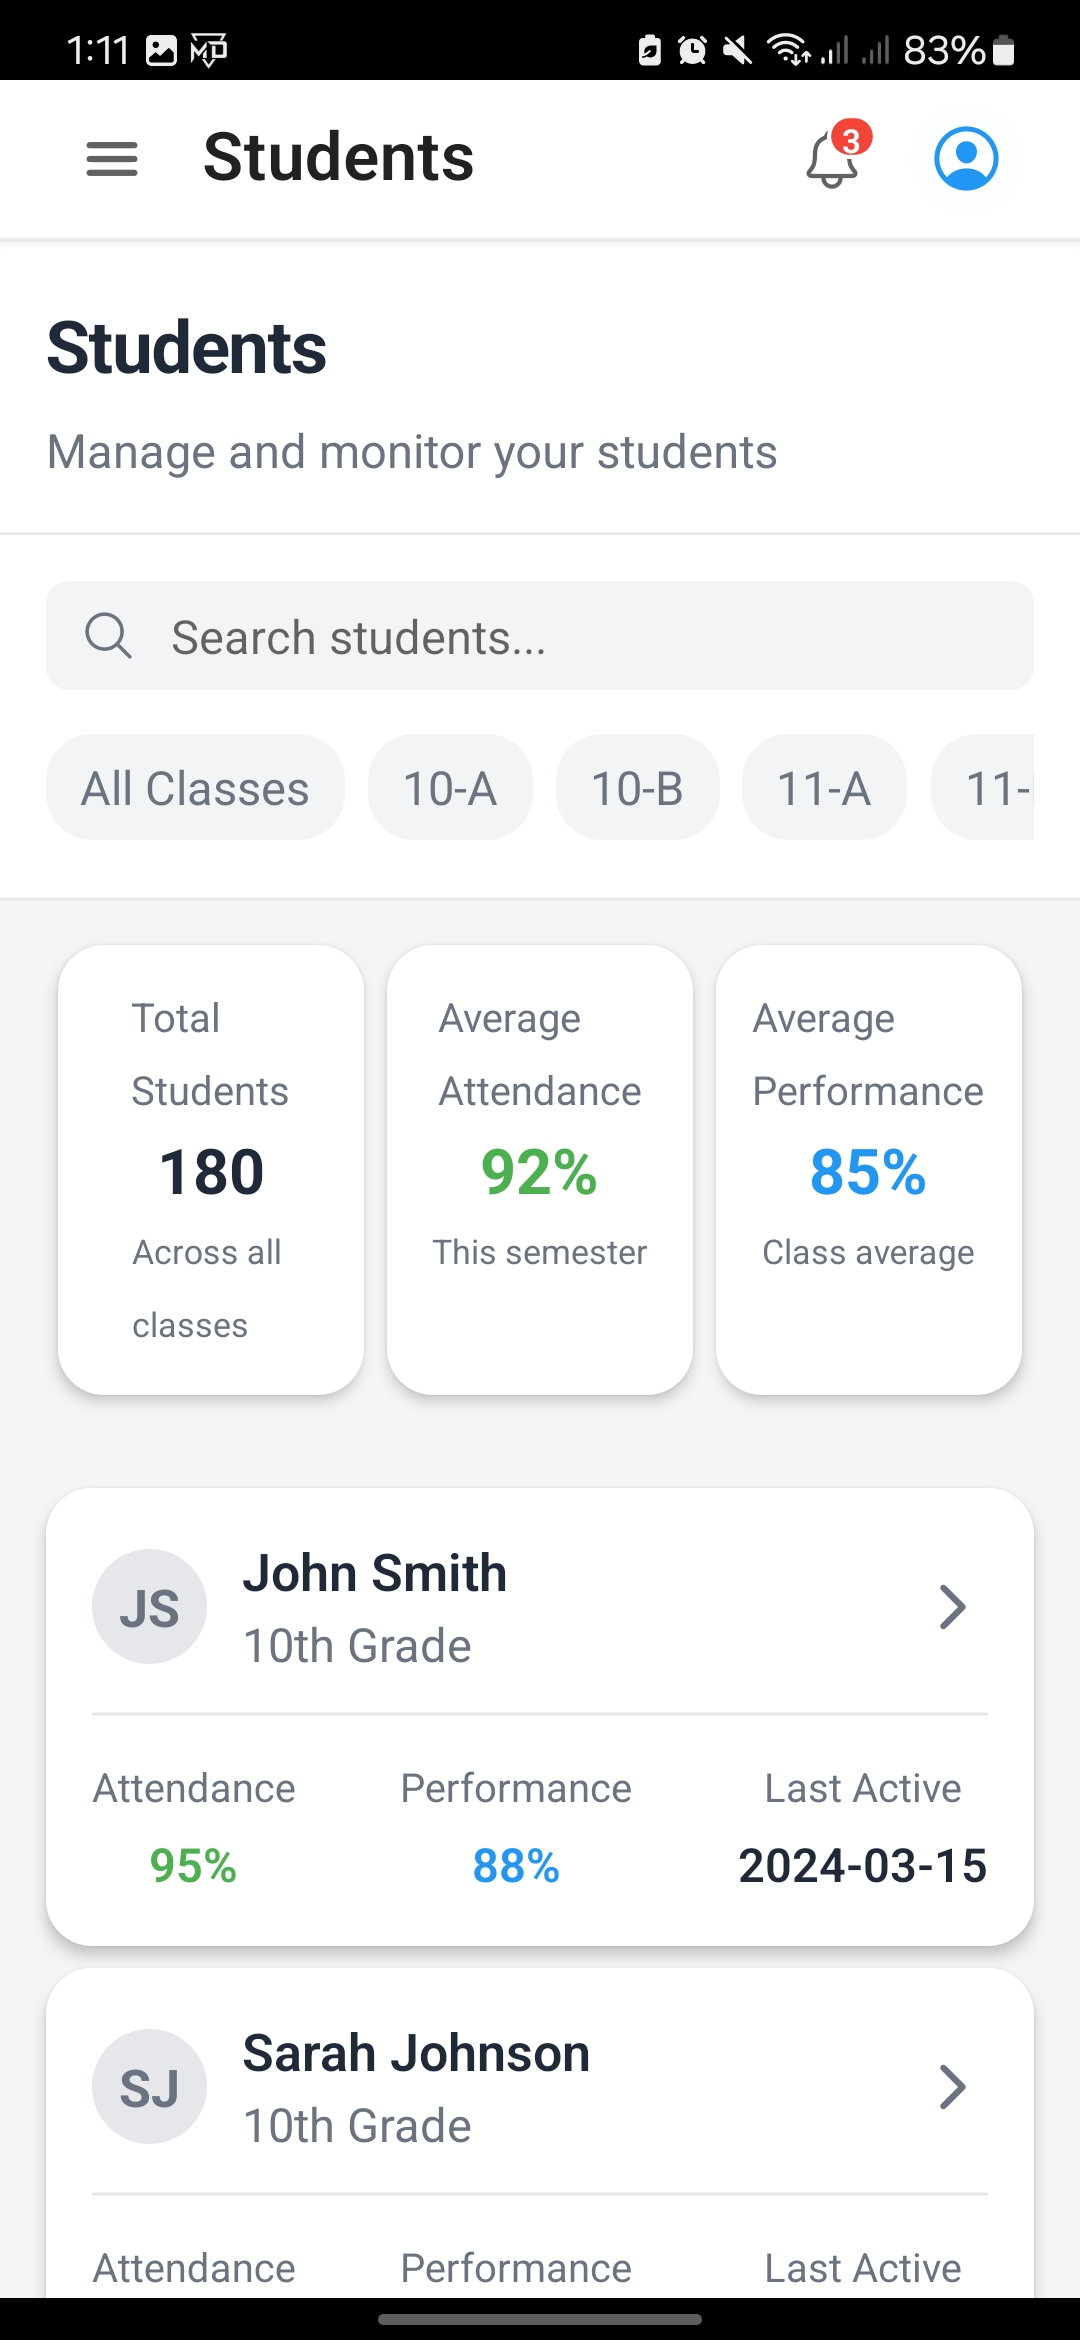
\includegraphics[width=0.4\textwidth,keepaspectratio]{pfe-pics/Mobile /Teacher/Screenshot_20250610_131112_Expo Go.jpg}
  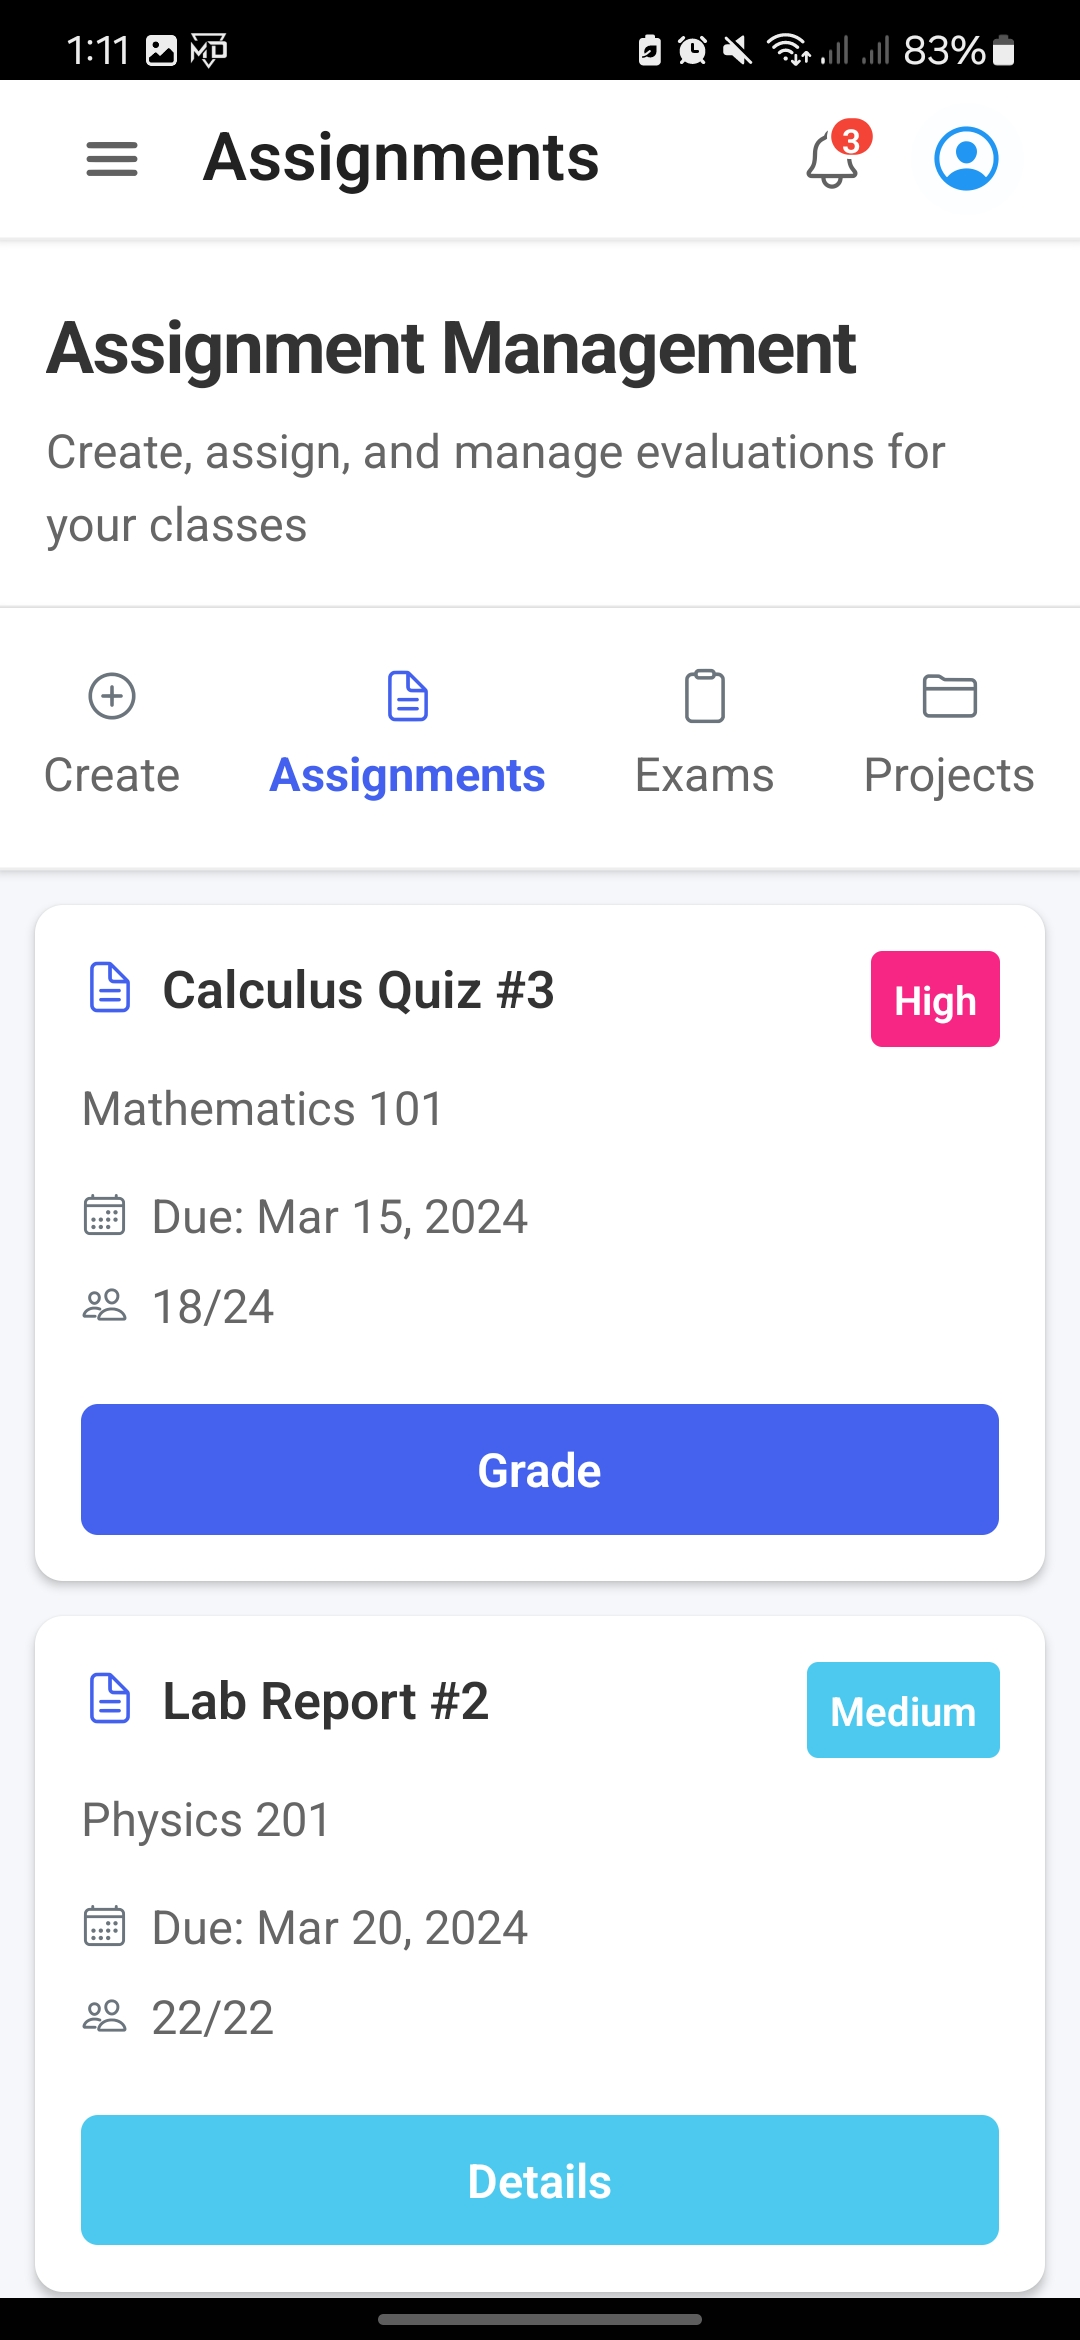
\includegraphics[width=0.4\textwidth,keepaspectratio]{pfe-pics/Mobile /Teacher/Screenshot_20250610_131132_Expo Go.jpg}
  \caption{\textbf{Interfaces de prise de présence et de notation} optimisées pour mobile.}
  \label{fig:mobile_teacher_attendance}
\end{figure}

\subsubsection{Interfaces mobiles pour les parents}

L'application mobile pour les parents facilite le suivi des activités scolaires de leurs enfants :

\begin{figure}[H]
  \centering
  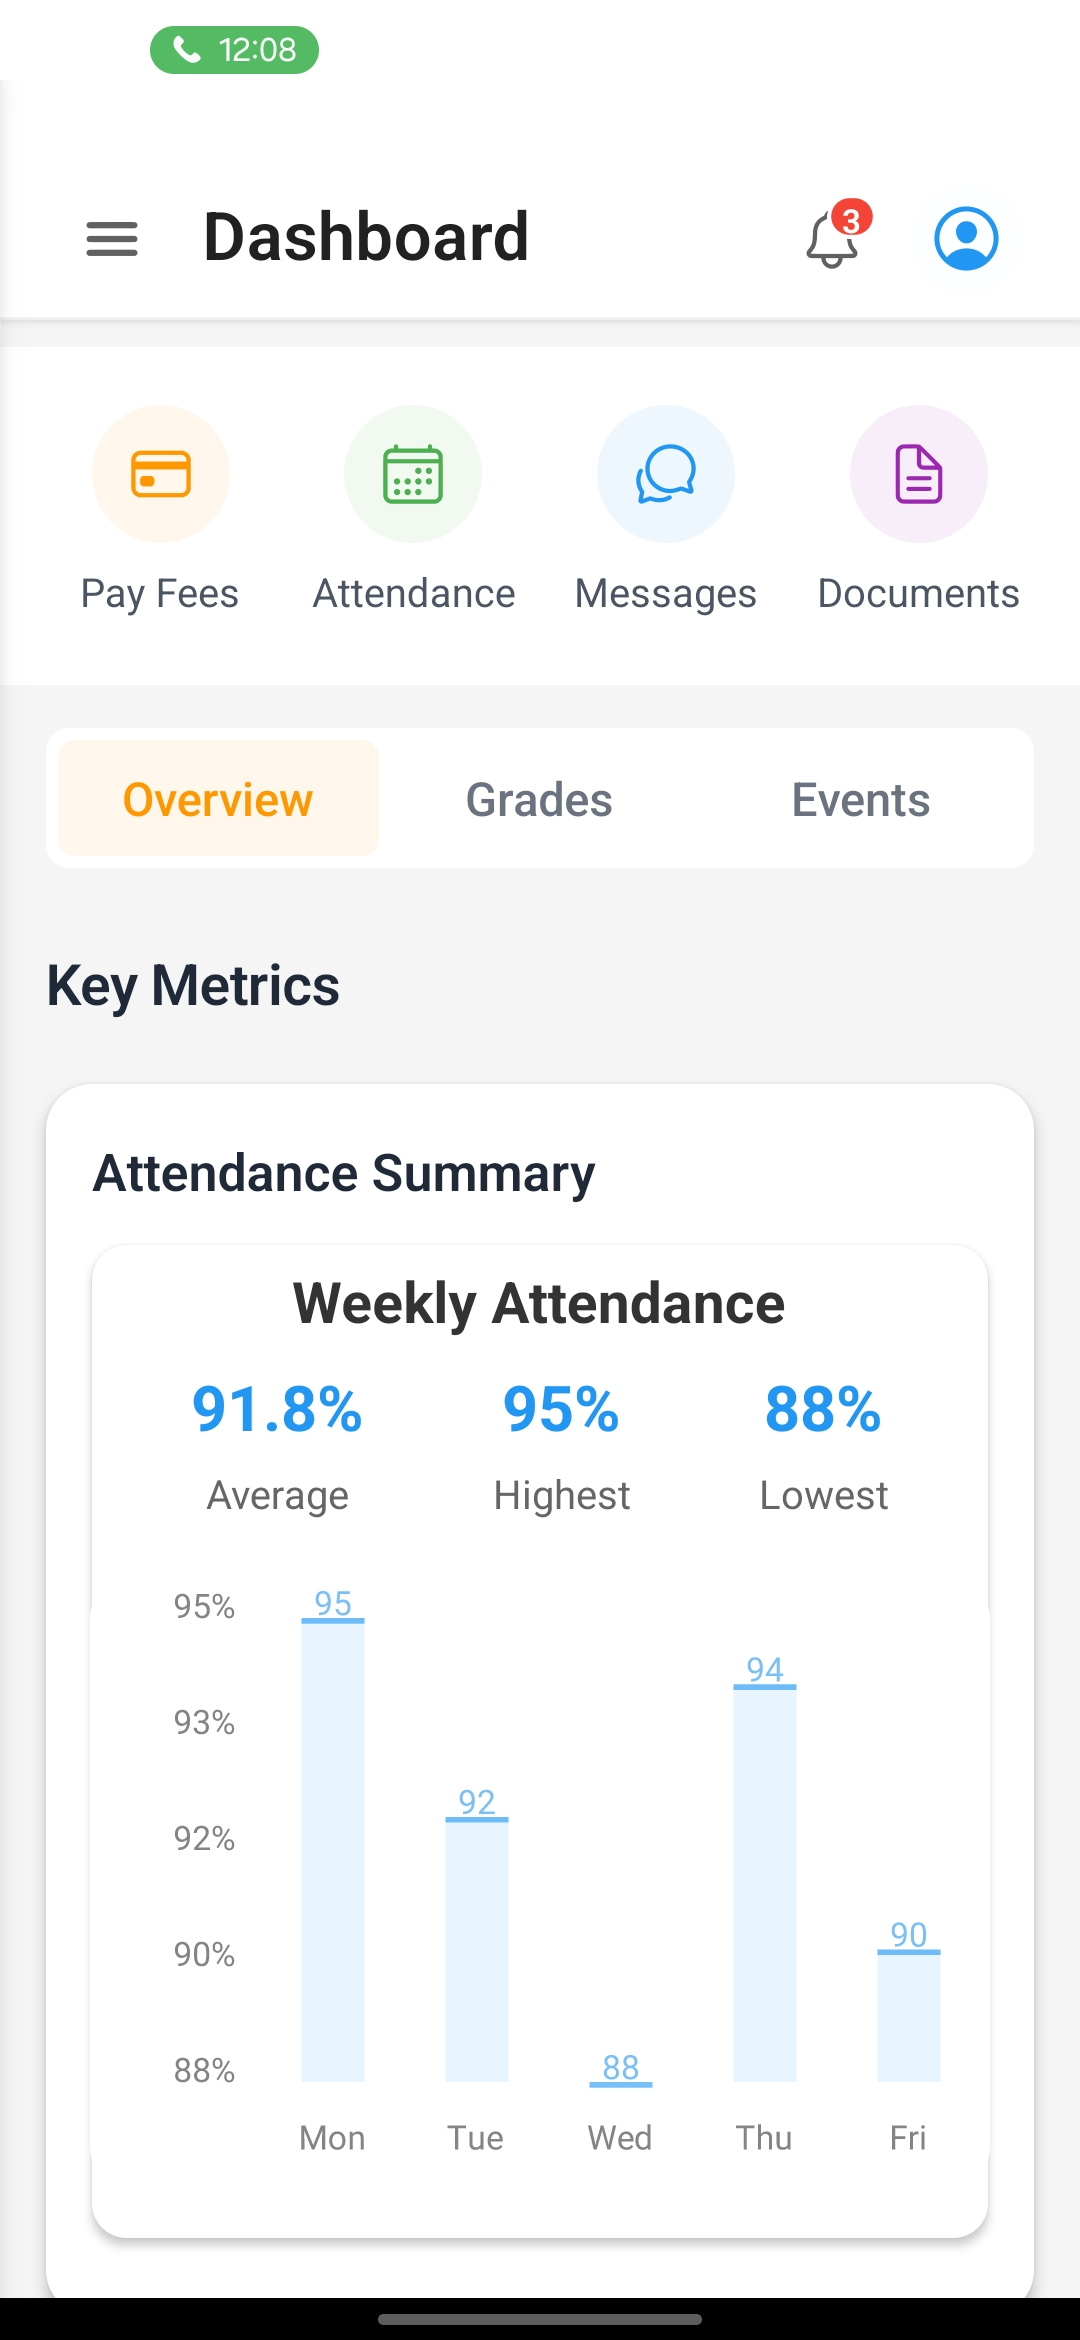
\includegraphics[width=0.4\textwidth,keepaspectratio]{pfe-pics/Mobile /Parent /Screenshot_20250610_132939_Expo Go.jpg}
  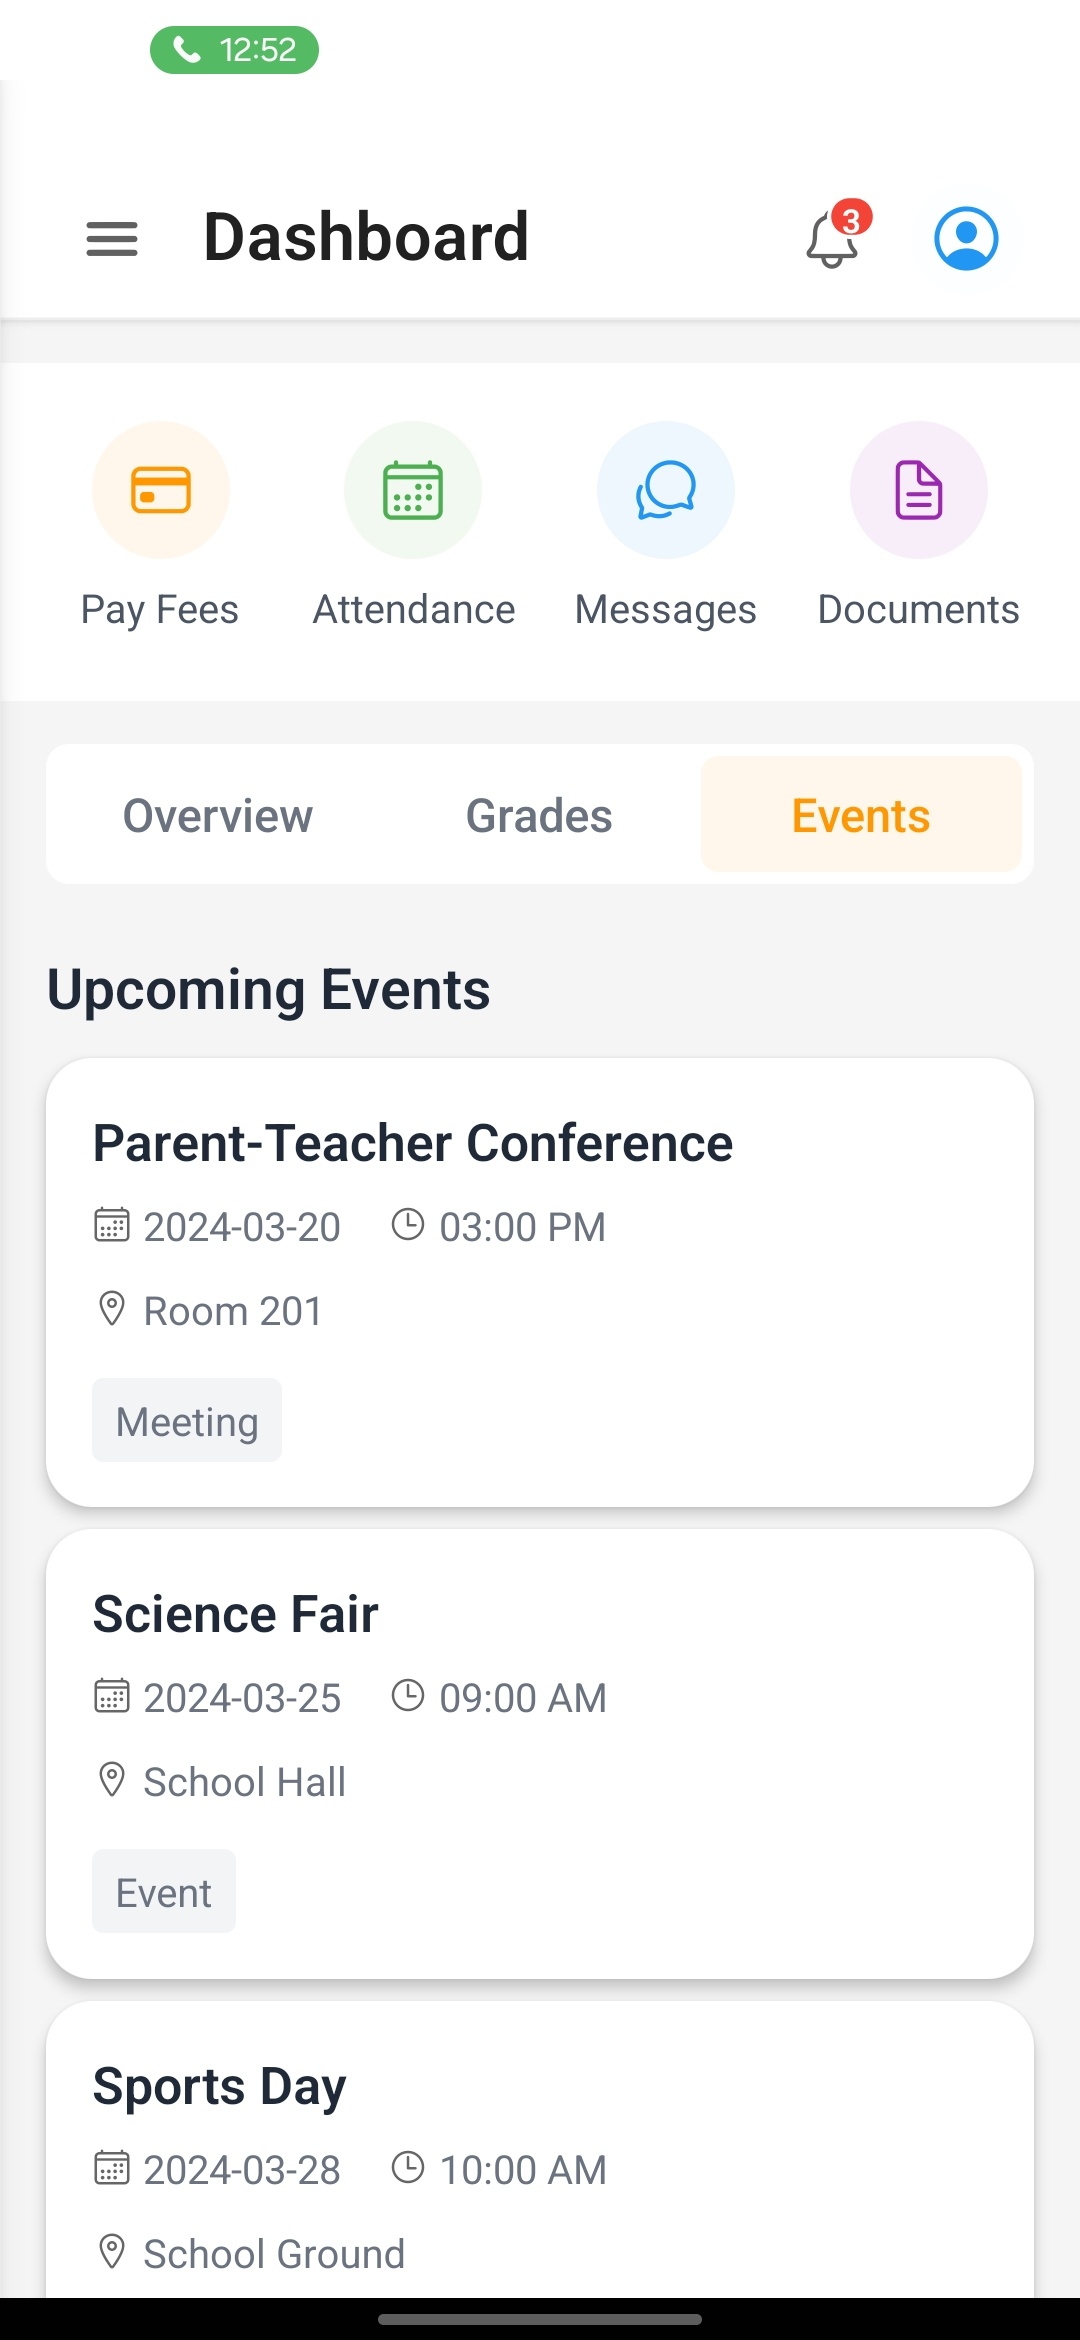
\includegraphics[width=0.4\textwidth,keepaspectratio]{pfe-pics/Mobile /Parent /Screenshot_20250610_133022_Expo Go.jpg}
  \caption{\textbf{Tableau de bord et sélection d'enfant} sur l'application mobile parent.}
  \label{fig:mobile_parent_dashboard}
\end{figure}

\begin{figure}[H]
  \centering
  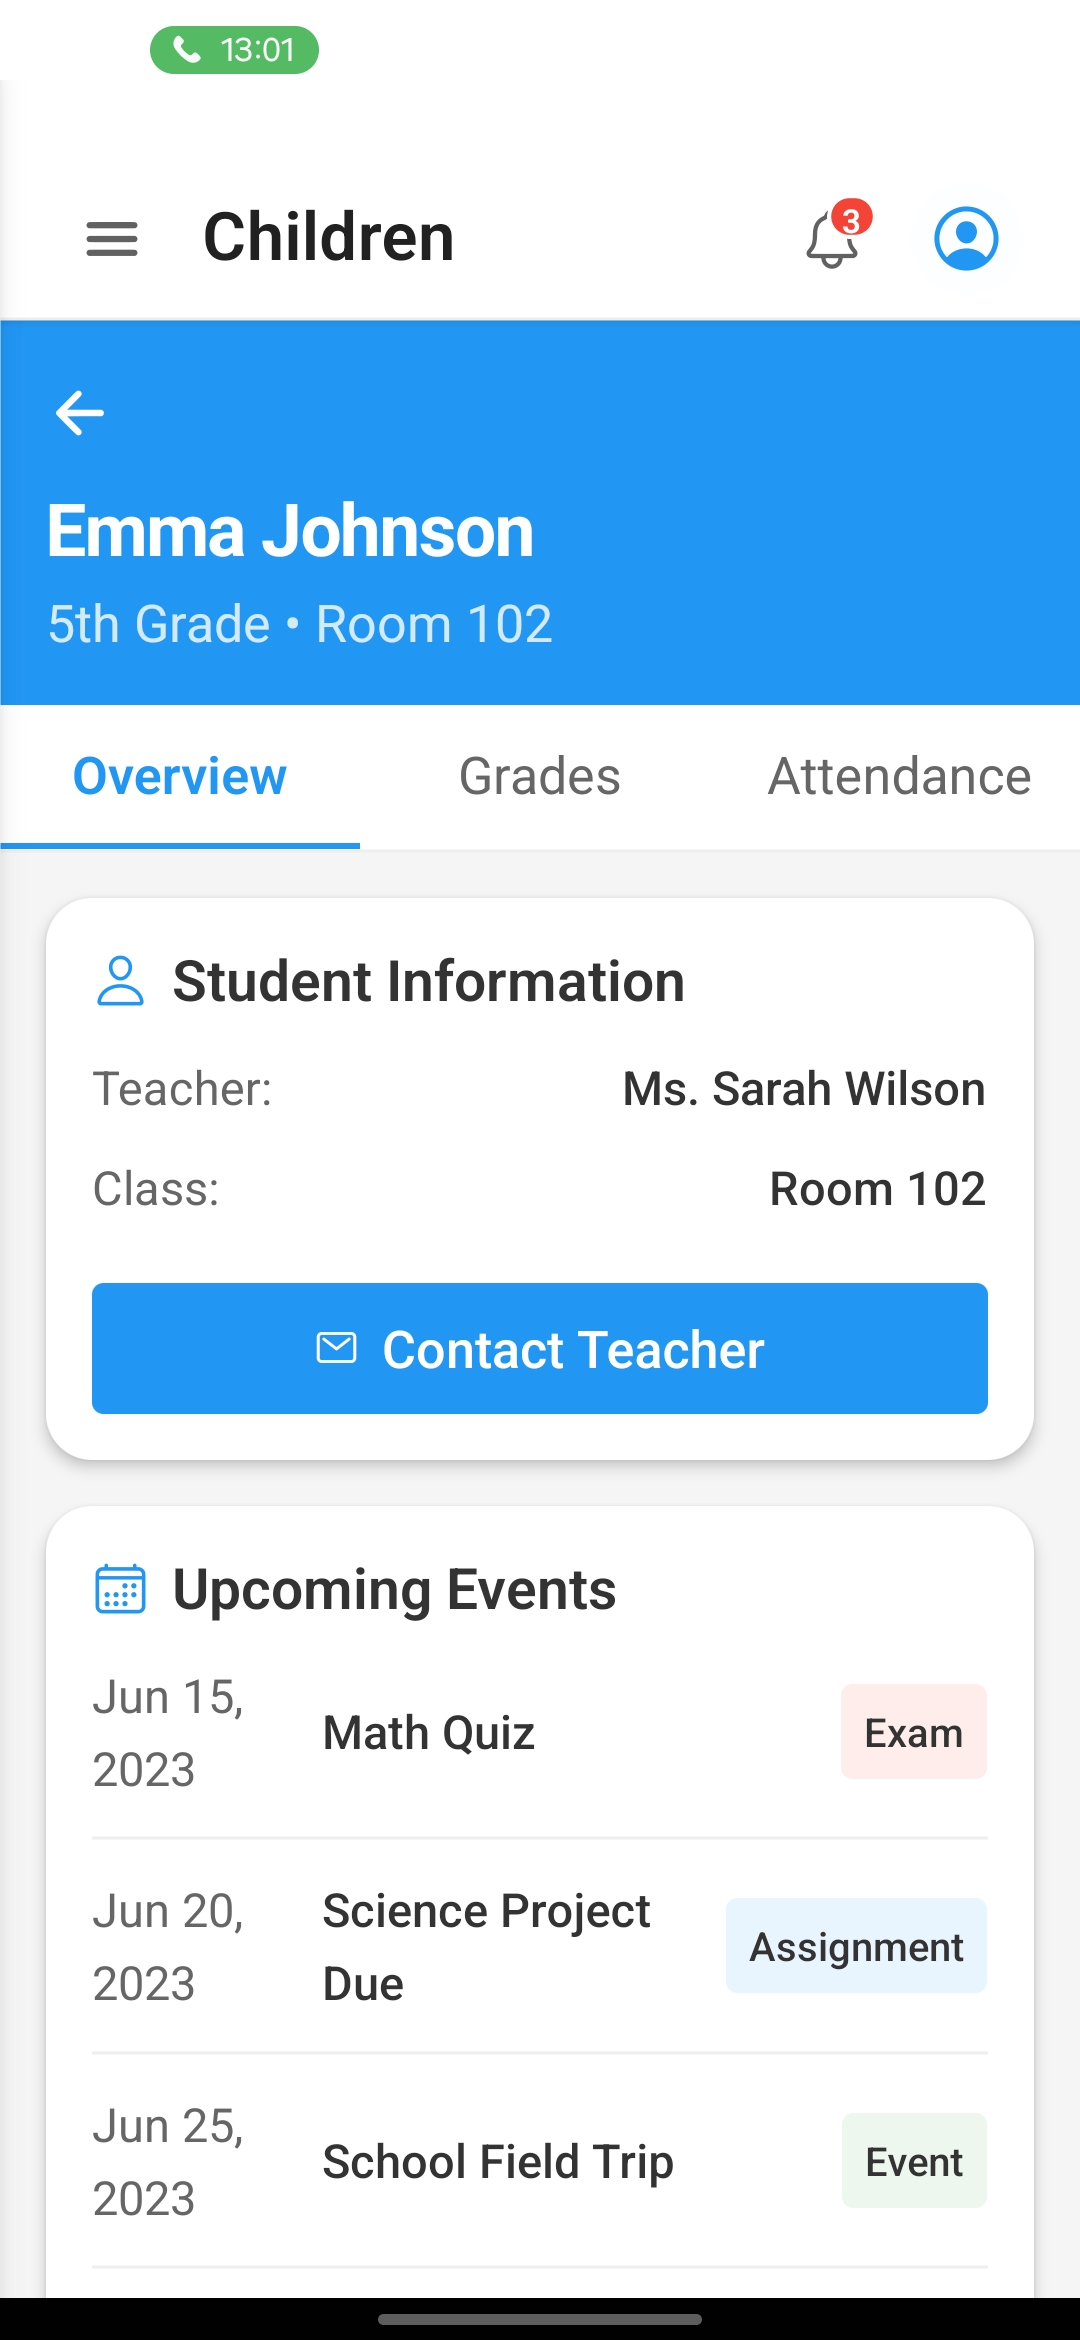
\includegraphics[width=0.4\textwidth,keepaspectratio]{pfe-pics/Mobile /Parent /Screenshot_20250610_133032_Expo Go.jpg}
  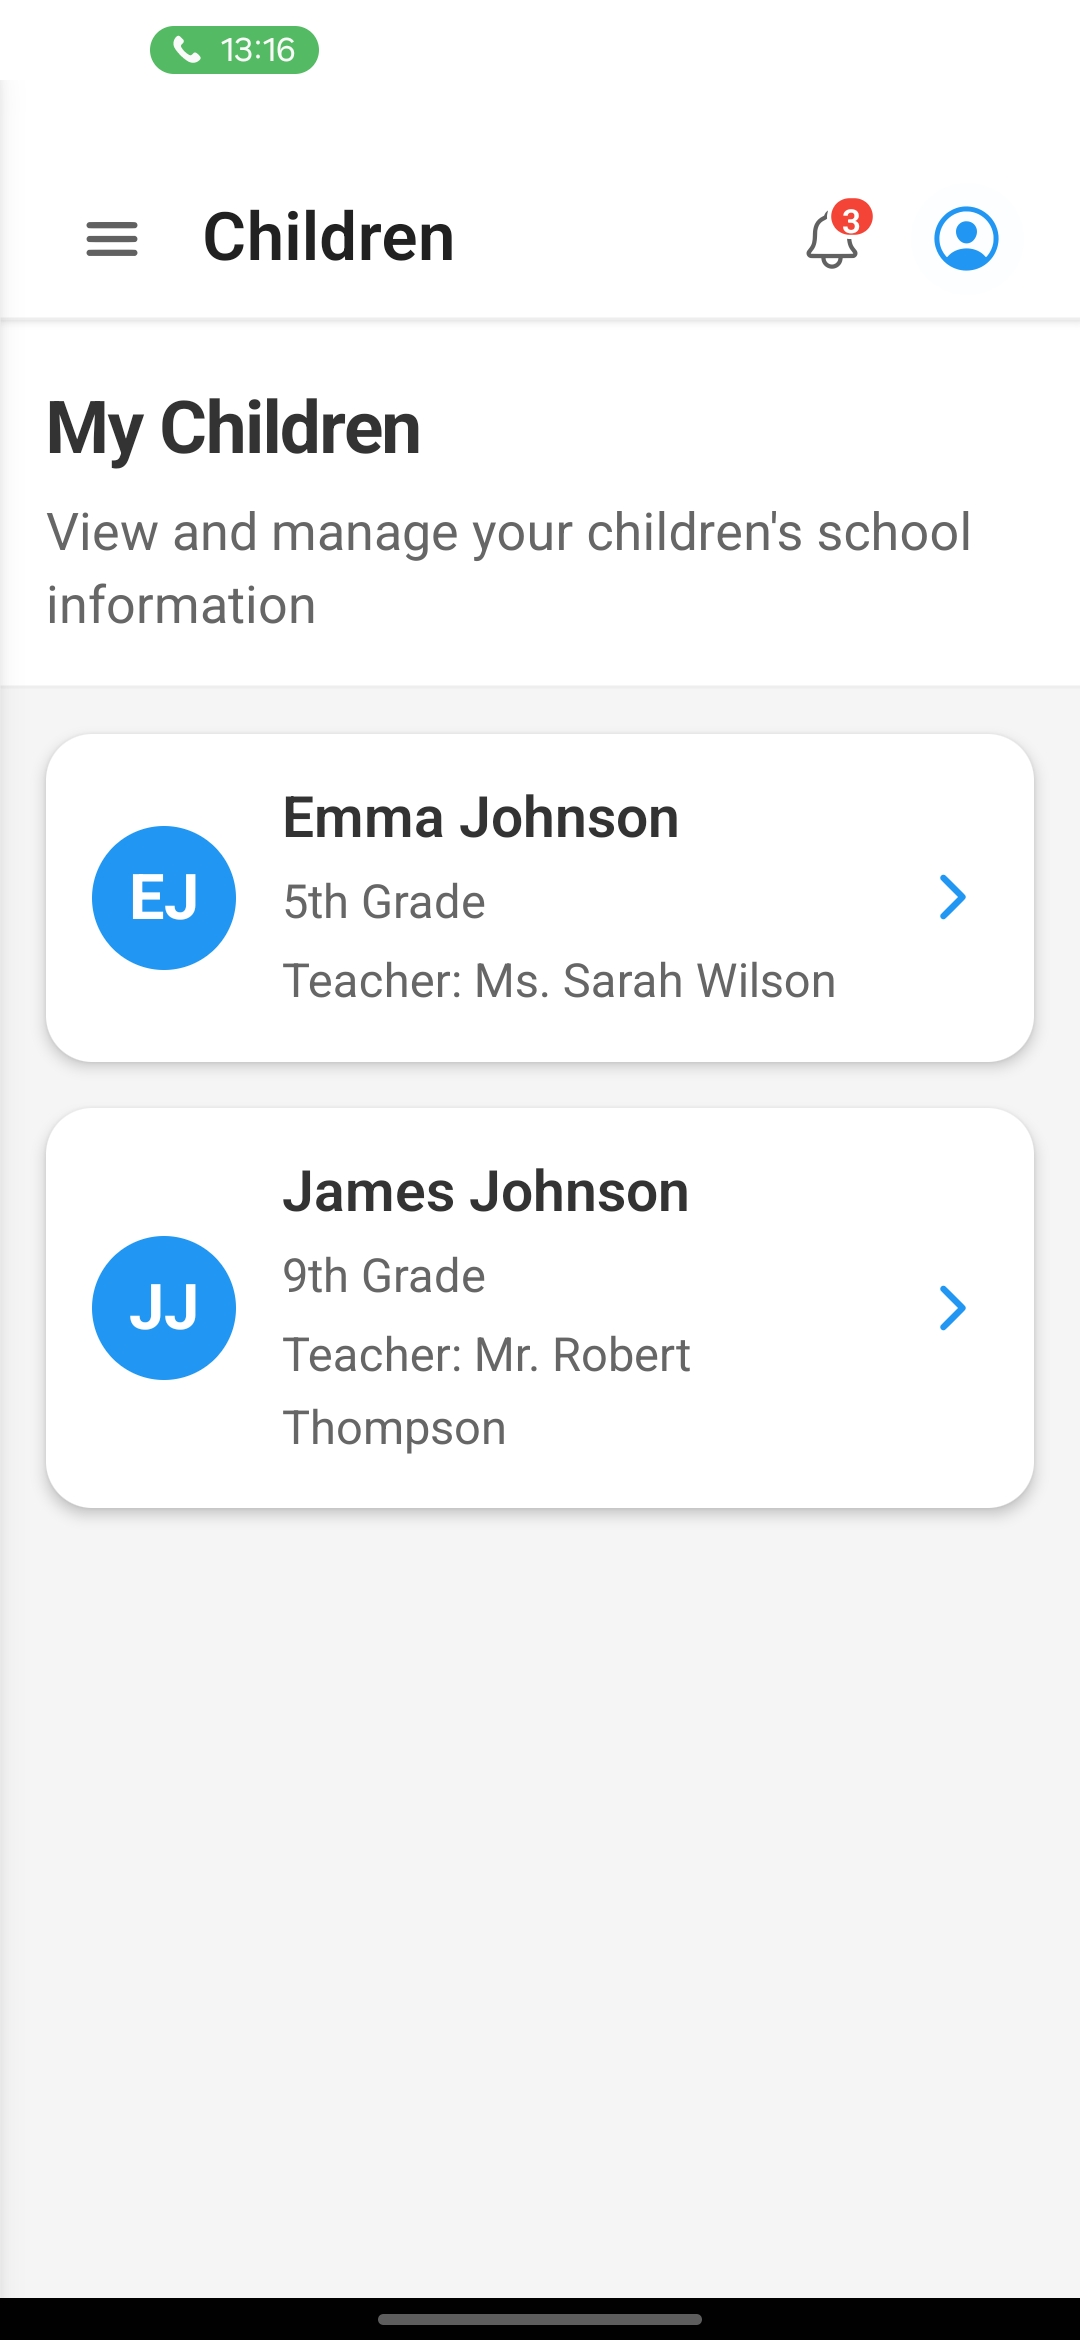
\includegraphics[width=0.4\textwidth,keepaspectratio]{pfe-pics/Mobile /Parent /Screenshot_20250610_133047_Expo Go.jpg}
  \caption{\textbf{Suivi des résultats et des présences} sur mobile pour les parents.}
  \label{fig:mobile_parent_monitoring}
\end{figure}

\subsubsection{Authentification mobile}

Le système d'authentification mobile offre une expérience sécurisée et conviviale :

\begin{figure}[H]
  \centering
  
\includegraphics[width=0.4\textwidth,keepaspectratio]{pfe-pics/Mobile /Auth/Screenshot_20250610_145348_Expo Go.jpg}
  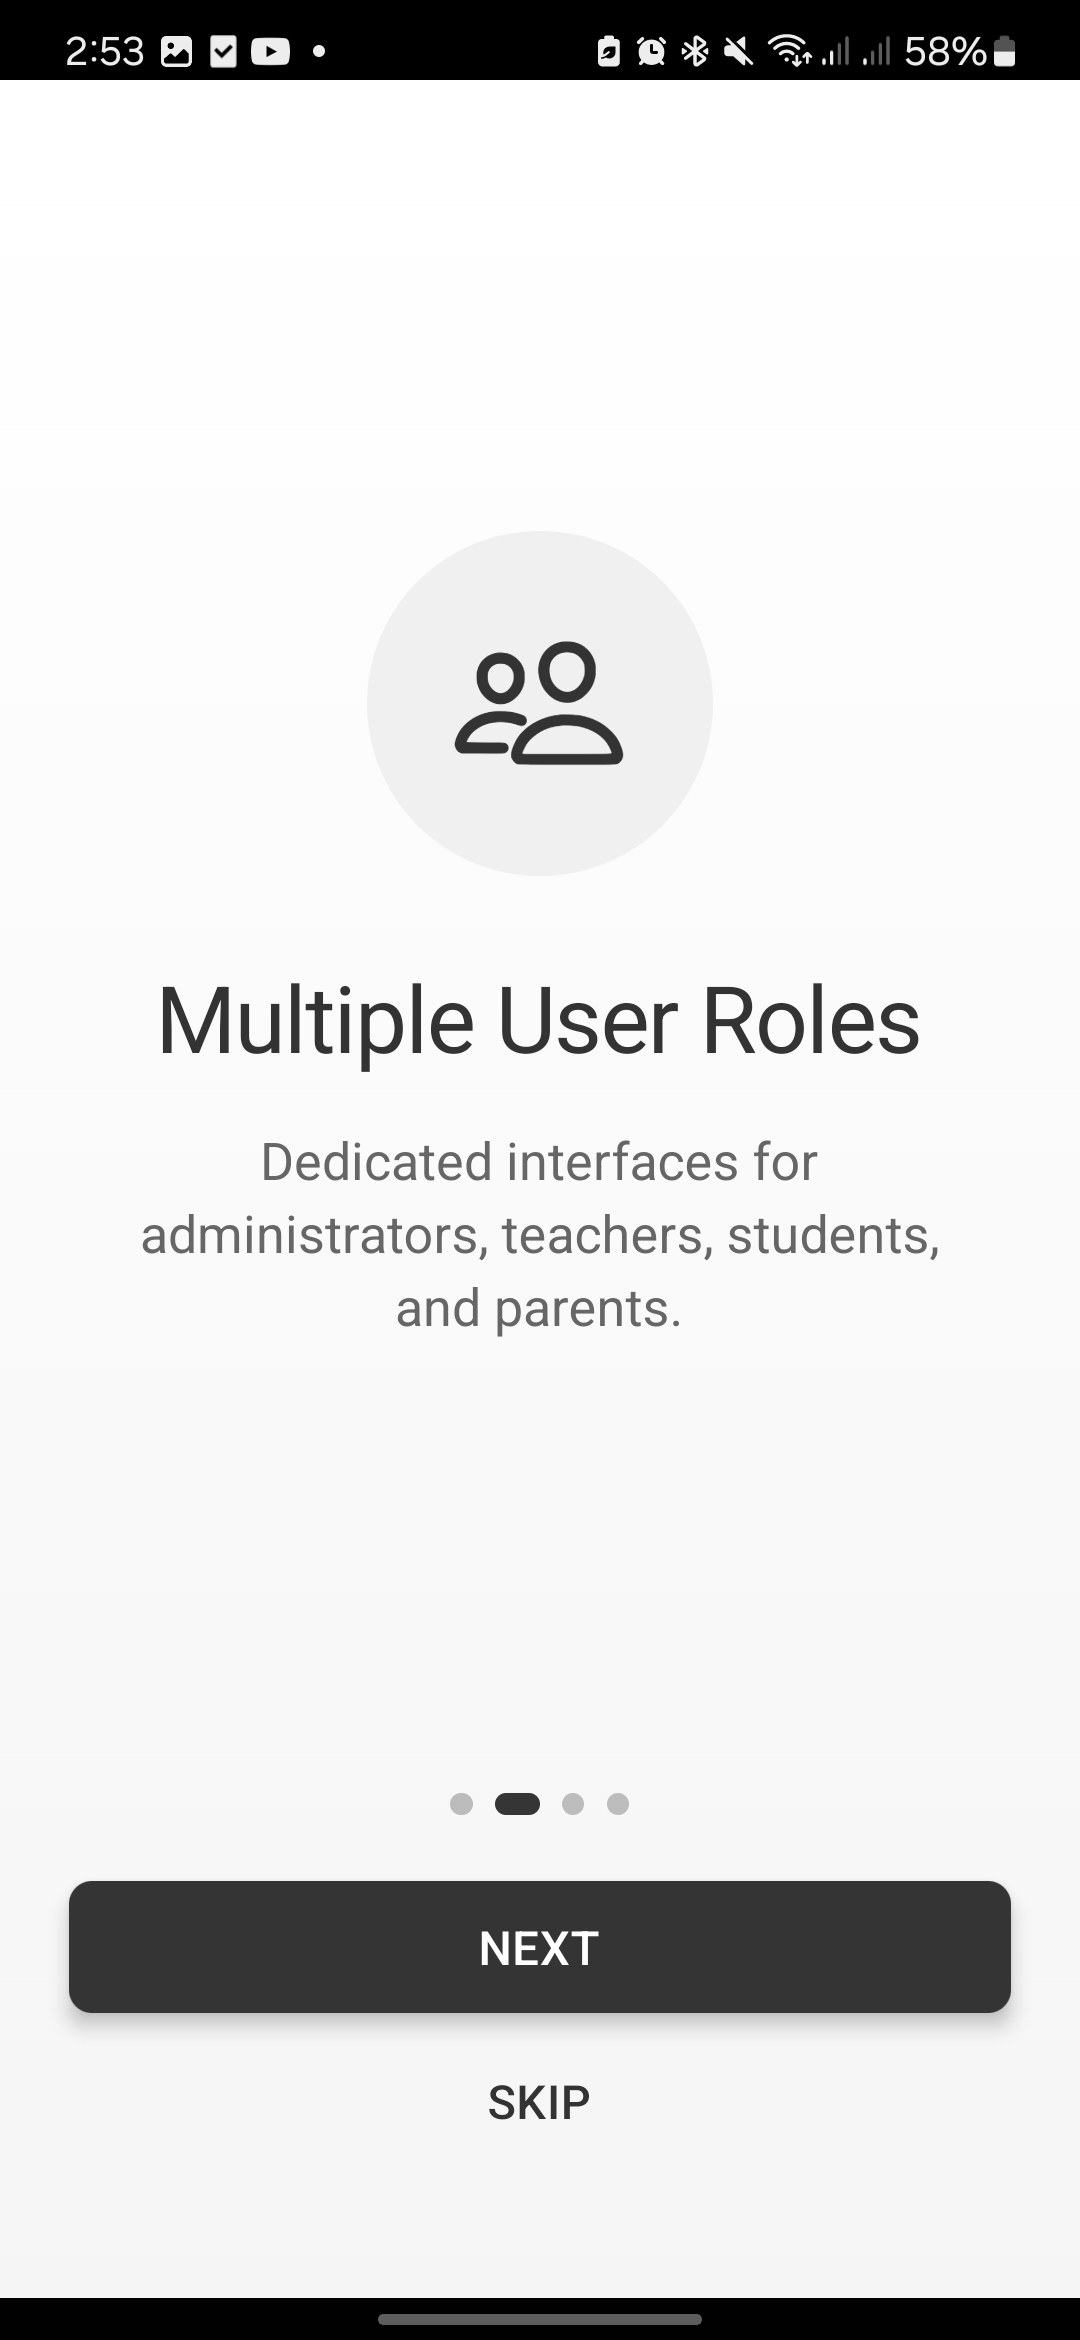
\includegraphics[width=0.4\textwidth,keepaspectratio]{pfe-pics/Mobile /Auth/Screenshot_20250610_145354_Expo Go.jpg}
  \caption{\textbf{Écrans de connexion et d'inscription} sur l'application mobile.}
  \label{fig:mobile_auth_screens}
\end{figure}

\section{Développement du système de création de profils IA}

Le développement du système de création de profils IA a représenté un défi technique particulier, combinant traitement de documents, intelligence artificielle et interfaces utilisateur intuitives.

\subsection{Implémentation du backend}

Le backend du système de création de profils IA a été développé avec FastAPI, un framework Python moderne offrant d'excellentes performances et une documentation automatique :

\begin{itemize}
  \item \textbf{Architecture API-first} : Conception d'une API RESTful complète comme fondation du système
  
  \item \textbf{Modèle de données} : Utilisation de Pydantic pour la validation et la sérialisation des données
  
  \item \textbf{Gestion asynchrone} : Implémentation d'opérations asynchrones pour optimiser les performances
  
  \item \textbf{Intégration avec OpenAI} : Connexion sécurisée avec l'API OpenAI via OpenRouter pour l'accès aux modèles de langage
  
  \item \textbf{Stockage hybride} : Combinaison de PostgreSQL pour les métadonnées et de stockage objet pour les documents
\end{itemize}

Voici un exemple de structure d'endpoint FastAPI pour la création d'un profil IA :

\begin{lstlisting}[style=codestyle, language=Python]
# app/routers/profiles.py
from fastapi import APIRouter, Depends, HTTPException, status
from sqlalchemy.ext.asyncio import AsyncSession
from typing import List

from app.schemas.profile import ProfileCreate, ProfileResponse
from app.services.profile_service import ProfileService
from app.dependencies import get_db, get_current_user
from app.models.user import User

router = APIRouter(prefix="/profiles", tags=["profiles"])

@router.post("/", response_model=ProfileResponse, status_code=status.HTTP_201_CREATED)
async def create_profile(
    profile_data: ProfileCreate,
    current_user: User = Depends(get_current_user),
    db: AsyncSession = Depends(get_db)
):
    profile_service = ProfileService(db)
    return await profile_service.create_profile(profile_data, current_user.id)

@router.get("/", response_model=List[ProfileResponse])
async def get_profiles(
    current_user: User = Depends(get_current_user),
    db: AsyncSession = Depends(get_db)
):
    profile_service = ProfileService(db)
    return await profile_service.get_user_profiles(current_user.id)
\end{lstlisting}

\subsection{Développement de l'interface utilisateur}

L'interface utilisateur du système de création de profils IA a été conçue pour être intuitive et efficace, permettant aux utilisateurs de créer et gérer facilement leurs profils IA :

\subsubsection{Page d'accueil et tableau de bord}

\begin{figure}[H]
  \centering
  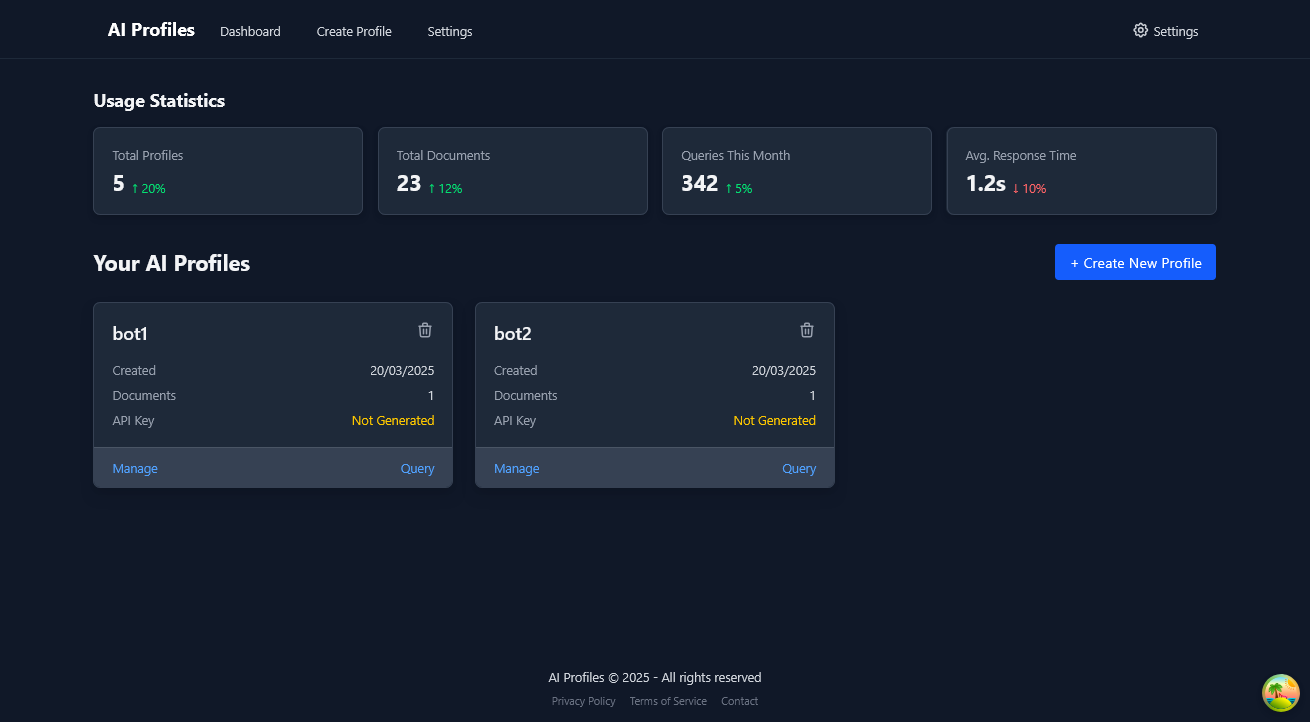
\includegraphics[width=0.85\textwidth,keepaspectratio]{pfe-pics/ai-profile-creation/dashboared_befor_adding_a_new_ai_profile.png}
  \caption{\textbf{Tableau de bord} du système de création de profils IA avant l'ajout d'un nouveau profil.}
  \label{fig:ai_dashboard}
\end{figure}

Le tableau de bord offre une vue d'ensemble des profils créés par l'utilisateur, avec des métriques clés comme :

\begin{itemize}
  \item Nombre de profils actifs
  \item Statistiques d'utilisation récente
  \item État de traitement des documents
  \item Accès rapide aux profils favoris
\end{itemize}

\subsubsection{Création et configuration de profil}

\begin{figure}[H]
  \centering
  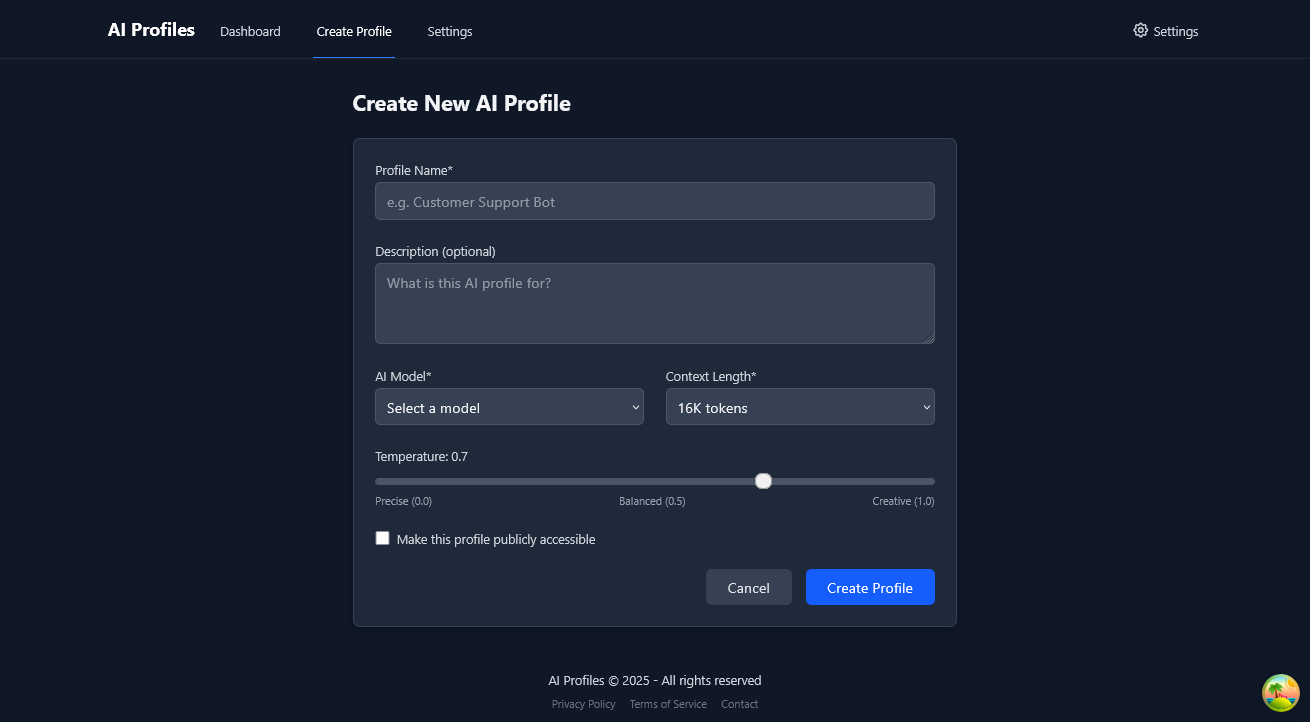
\includegraphics[width=0.85\textwidth,keepaspectratio]{pfe-pics/ai-profile-creation/creating_and_ai_prifile.png}
  \caption{\textbf{Interface de création de profil IA} avec options de configuration.}
  \label{fig:profile_creation}
\end{figure}

L'interface de création de profil permet aux utilisateurs de :

\begin{itemize}
  \item Définir les informations de base du profil (nom, description, domaine)
  \item Configurer le comportement de l'IA (ton, style de réponse, niveau de détail)
  \item Sélectionner des catégories et tags pour organiser les profils
  \item Définir les paramètres de confidentialité et d'accès
\end{itemize}

\subsubsection{Upload et gestion des documents}

\begin{figure}[H]
  \centering
  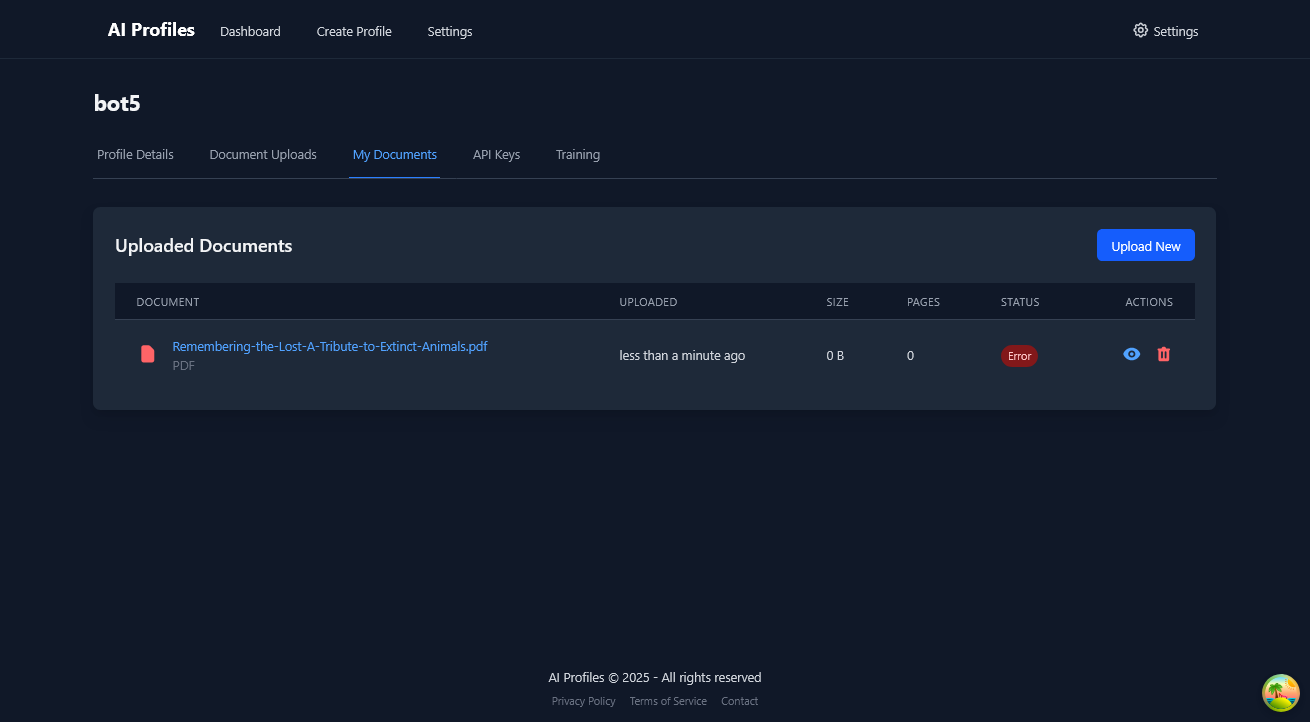
\includegraphics[width=0.85\textwidth,keepaspectratio]{pfe-pics/ai-profile-creation/see_upladed_documents_knoladge.png}
  \caption{\textbf{Interface de visualisation des documents uploadés} et leur connaissance associée.}
  \label{fig:document_knowledge}
\end{figure}

\begin{figure}[H]
  \centering
  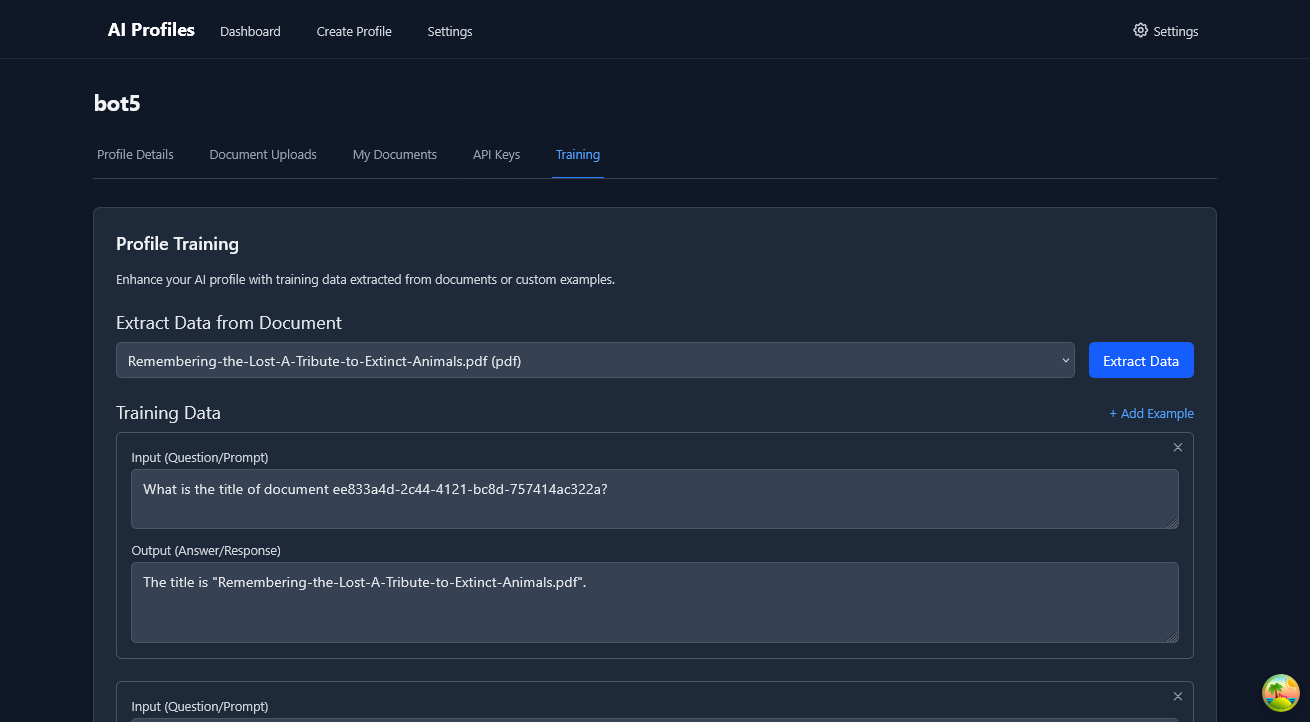
\includegraphics[width=0.85\textwidth,keepaspectratio]{pfe-pics/ai-profile-creation/extract_info_from_file_and_training_pfrile.png}
  \caption{\textbf{Interface d'extraction d'information} à partir des fichiers et entrainement du profil.}
  \label{fig:document_extraction}
\end{figure}

L'interface de gestion des documents offre des fonctionnalités avancées :

\begin{itemize}
  \item Upload par glisser-déposer de multiples formats (PDF, DOCX, TXT)
  \item Visualisation de l'état de traitement en temps réel
  \item Organisation des documents par catégories
  \item Prévisualisation du contenu extrait
  \item Possibilité d'ajouter des métadonnées et annotations
\end{itemize}

\begin{figure}[H]
  \centering
  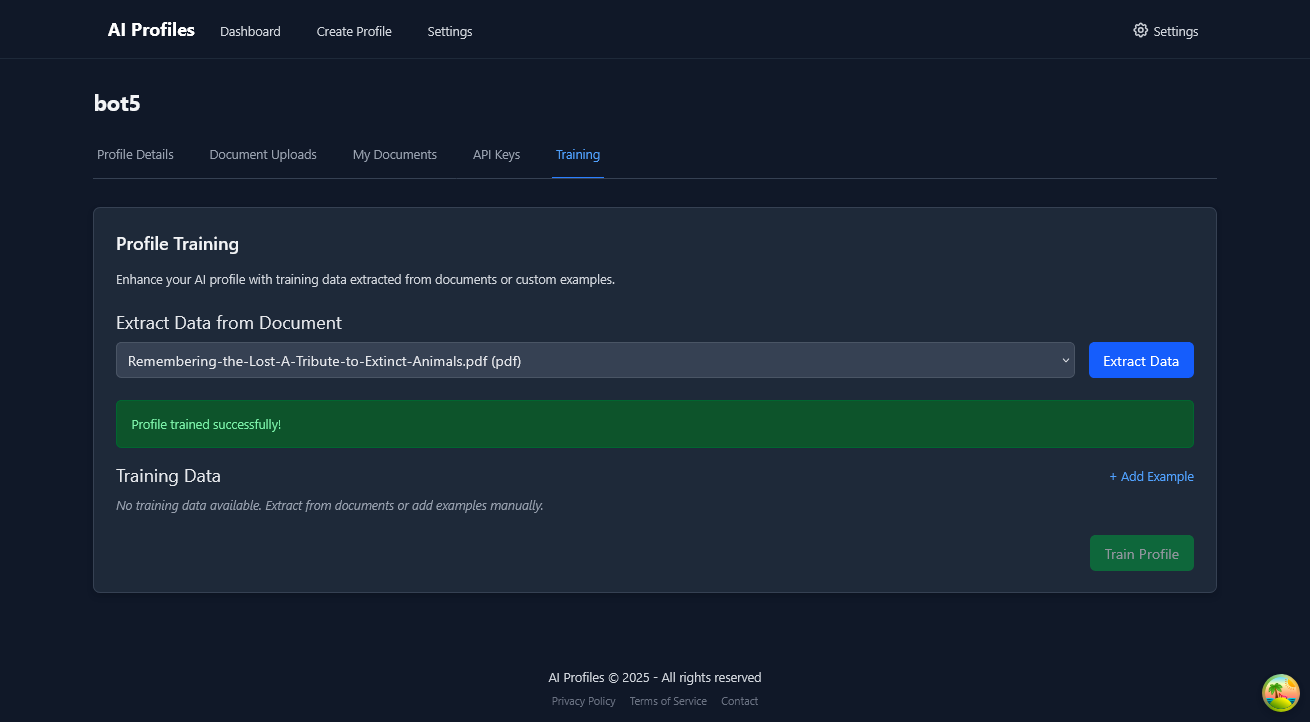
\includegraphics[width=0.85\textwidth,keepaspectratio]{pfe-pics/ai-profile-creation/succesful_knoladge_integration.png}
  \caption{\textbf{Confirmation d'intégration réussie} des connaissances extraites dans le profil IA.}
  \label{fig:knowledge_integration}
\end{figure}

\subsubsection{Interface de test et conversation}

\begin{figure}[H]
  \centering
  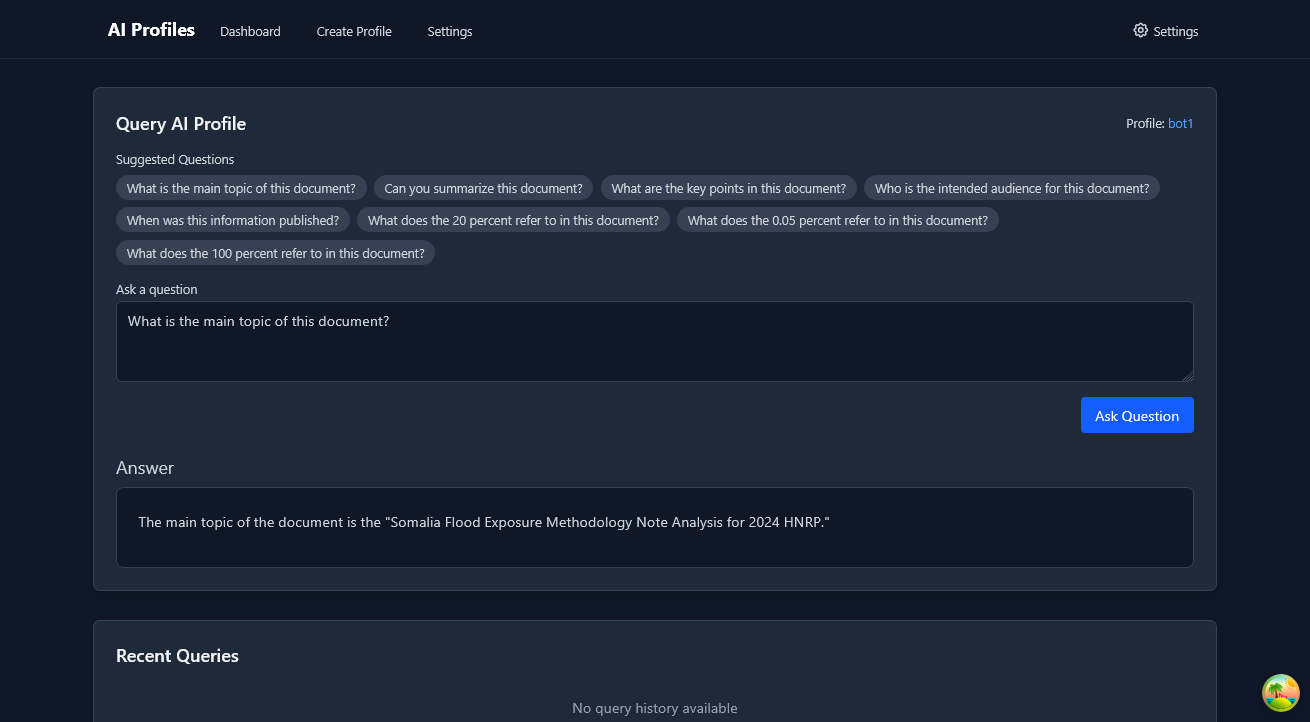
\includegraphics[width=0.85\textwidth,keepaspectratio]{pfe-pics/ai-profile-creation/chat_interface_to_test_the_profile.png}
  \caption{\textbf{Interface de conversation pour tester le profil IA} créé.}
  \label{fig:profile_testing}
\end{figure}

\begin{figure}[H]
  \centering
  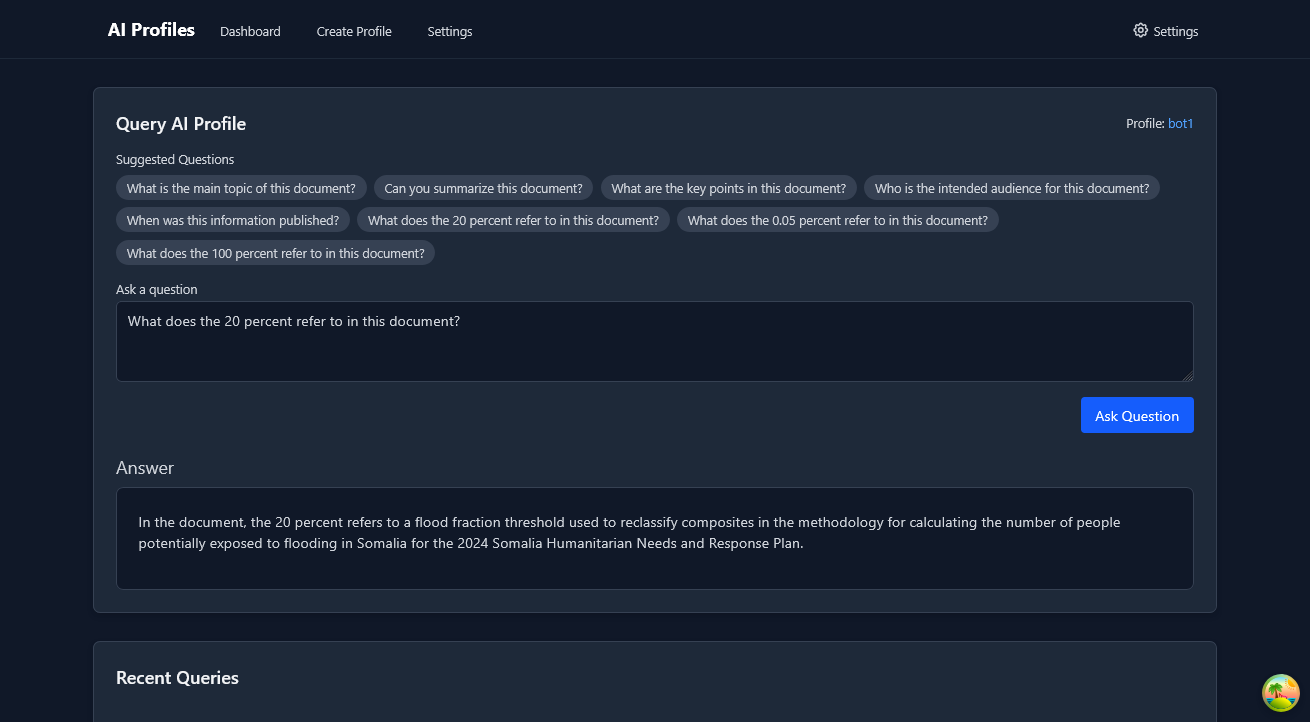
\includegraphics[width=0.85\textwidth,keepaspectratio]{pfe-pics/ai-profile-creation/chat_interface_for_testing_profile_2_test_prompt_succes.png}
  \caption{\textbf{Résultat réussi de test du profil} avec des prompts de vérification.}
  \label{fig:profile_test_success}
\end{figure}

L'interface de conversation permet une interaction naturelle avec les profils IA :

\begin{itemize}
  \item Design inspiré des applications de messagerie modernes
  \item Historique des conversations sauvegardé
  \item Affichage des sources documentaires pour les réponses
  \item Options de feedback pour améliorer les réponses
  \item Possibilité de partager des conversations
\end{itemize}

\subsubsection{Gestion des API et intégrations}

\begin{figure}[H]
  \centering
  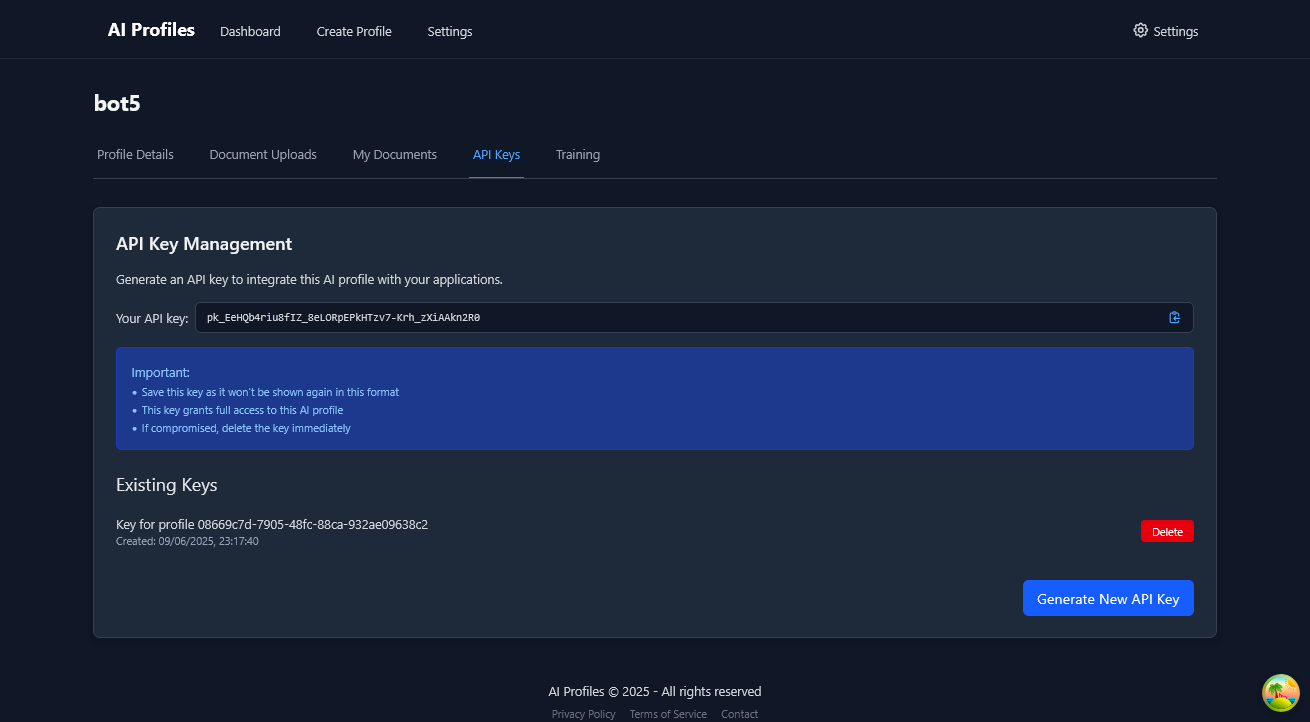
\includegraphics[width=0.85\textwidth,keepaspectratio]{pfe-pics/ai-profile-creation/create_and_api_key_for_trained_profile.png}
  \caption{\textbf{Interface de création de clé API} pour un profil IA entrainé.}
  \label{fig:api_key_creation}
\end{figure}

\begin{figure}[H]
  \centering
  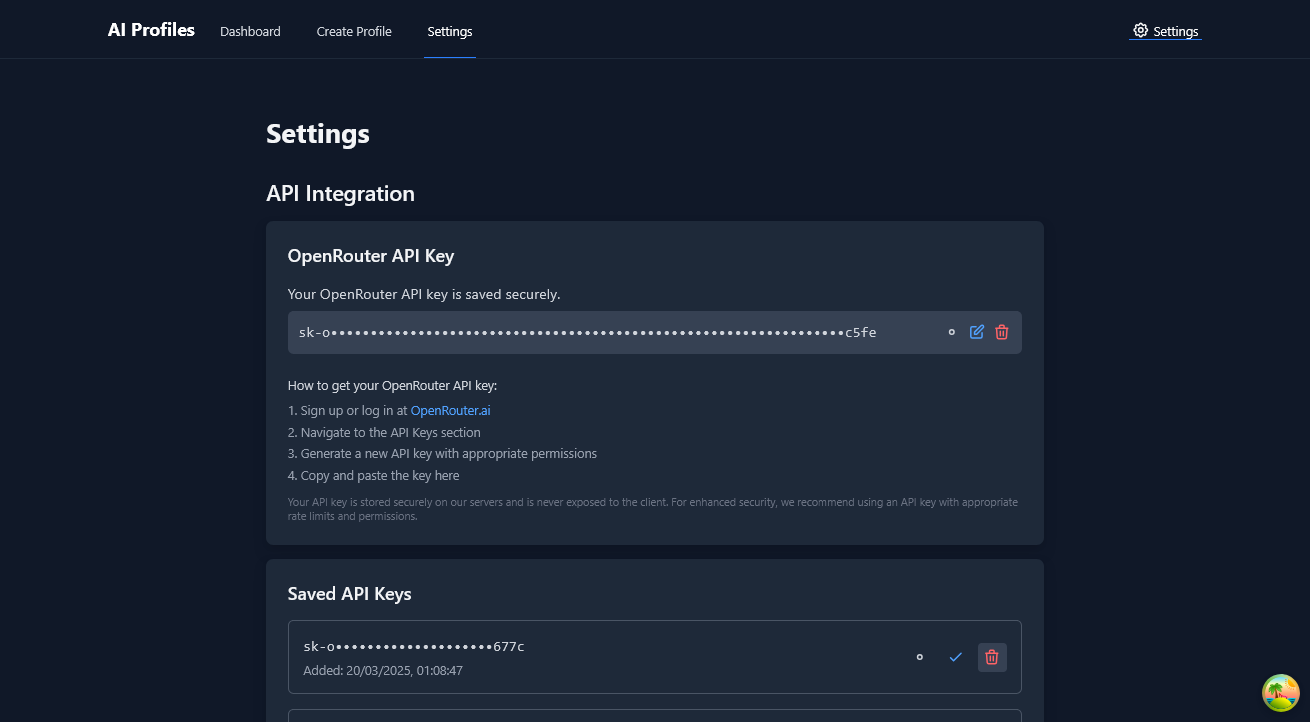
\includegraphics[width=0.85\textwidth,keepaspectratio]{pfe-pics/ai-profile-creation/adding_openRouter_api.png}
  \caption{\textbf{Interface d'ajout d'une clé API OpenRouter} pour l'accès aux modèles de langage.}
  \label{fig:openrouter_api_addition}
\end{figure}

\begin{figure}[H]
  \centering
  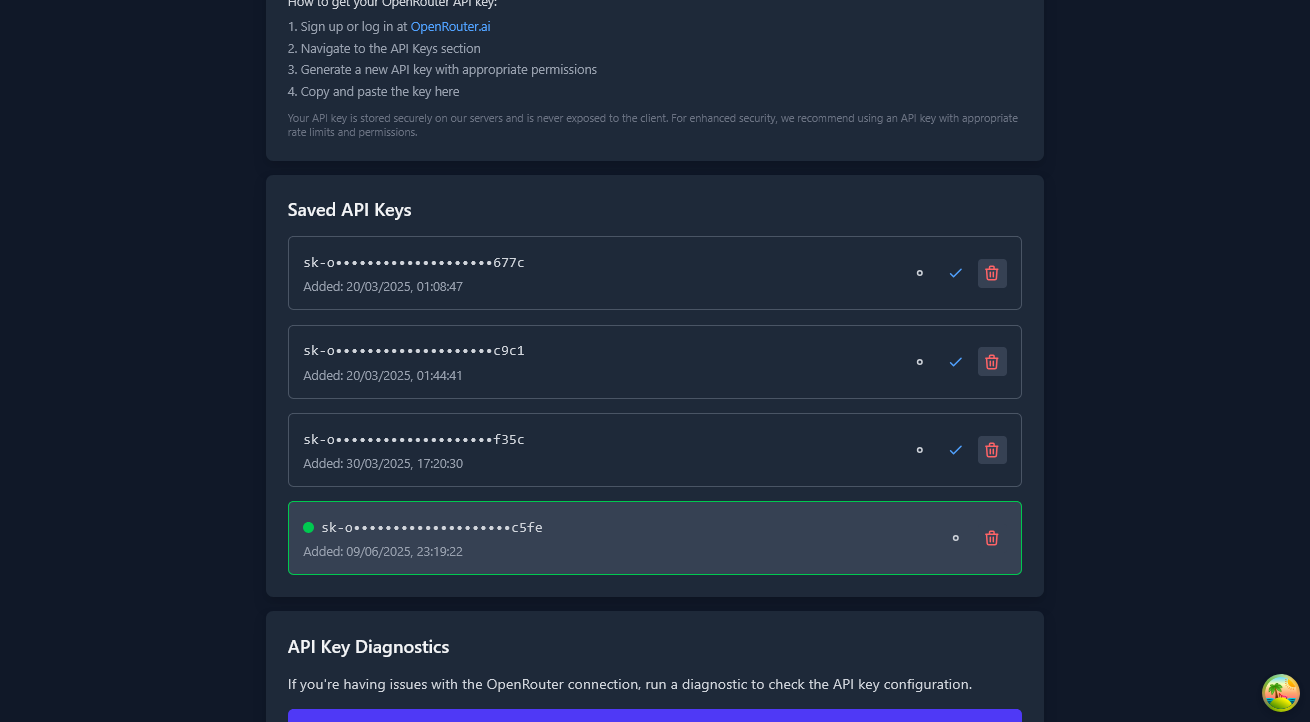
\includegraphics[width=0.85\textwidth,keepaspectratio]{pfe-pics/ai-profile-creation/oneRouter_keys_hestory.png}
  \caption{\textbf{Historique des clés API OpenRouter} utilisées par le système.}
  \label{fig:api_keys_history}
\end{figure}

Pour les utilisateurs souhaitant intégrer leurs profils IA dans d'autres applications :

\begin{itemize}
  \item Création et gestion de clés API avec permissions spécifiques
  \item Documentation interactive des endpoints disponibles
  \item Exemples de code pour différents langages de programmation
  \item Suivi de l'utilisation et des quotas
\end{itemize}

\begin{figure}[H]
  \centering
  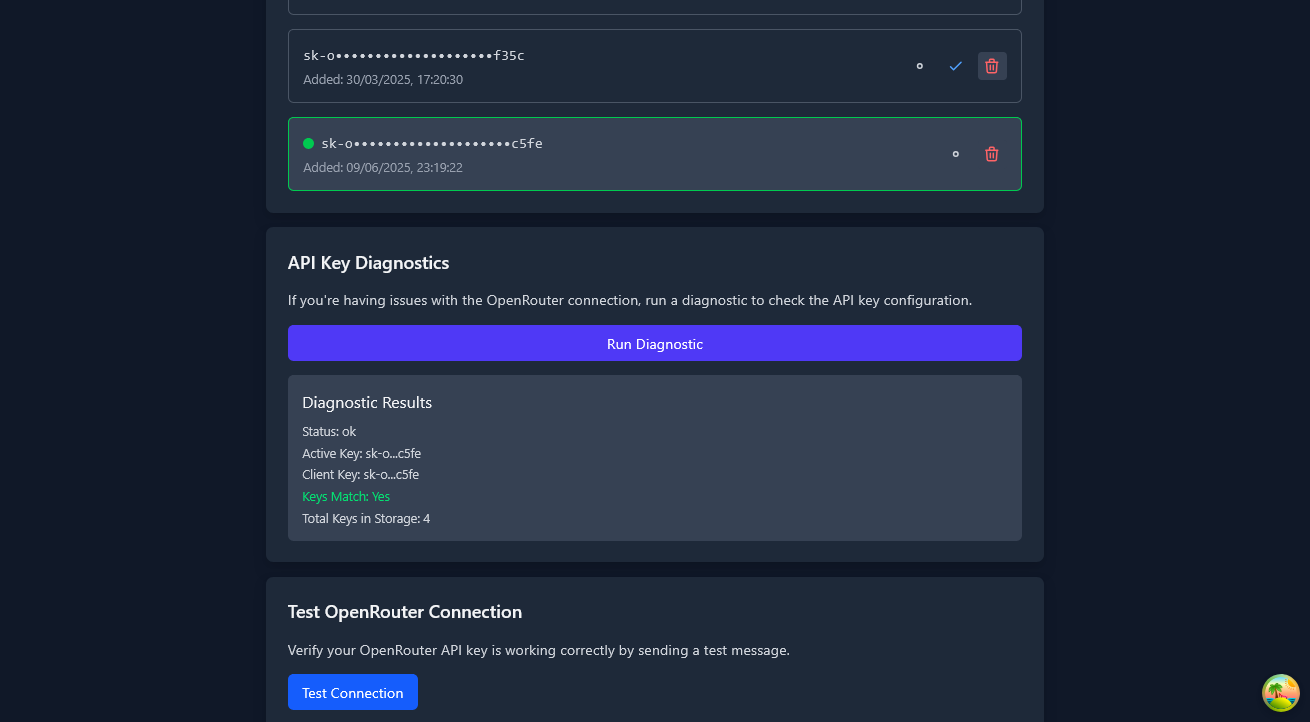
\includegraphics[width=0.85\textwidth,keepaspectratio]{pfe-pics/ai-profile-creation/api_diagnostics.png}
  \caption{\textbf{Interface de diagnostics API} pour la vérification des problèmes d'intégration.}
  \label{fig:api_diagnostics}
\end{figure}

\begin{figure}[H]
  \centering
  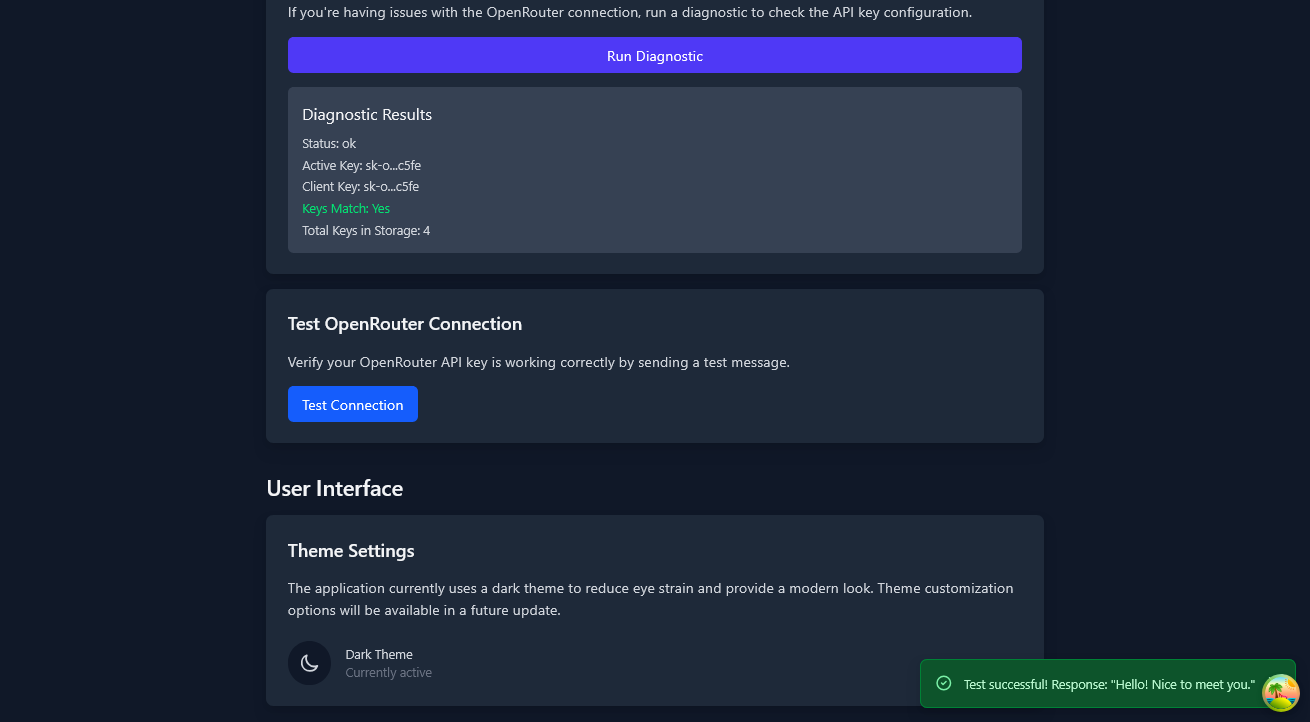
\includegraphics[width=0.85\textwidth,keepaspectratio]{pfe-pics/ai-profile-creation/test_openRouter_connection.png}
  \caption{\textbf{Test de connexion OpenRouter} pour vérifier la configuration du service.}
  \label{fig:openrouter_test}
\end{figure}

\subsection{Pipeline de traitement des documents}

Le cœur du système de création de profils IA réside dans son pipeline de traitement des documents, qui transforme les documents bruts en base de connaissances structurée pour l'IA.

\subsubsection{Architecture du pipeline}

Le pipeline de traitement a été conçu comme un système asynchrone à plusieurs étapes :

\begin{itemize}
  \item \textbf{Réception et validation} : Vérification des formats et de l'intégrité des documents
  
  \item \textbf{Extraction de texte} : Conversion des différents formats en texte brut
  
  \item \textbf{Analyse structurelle} : Identification des sections, titres et éléments spéciaux
  
  \item \textbf{Segmentation intelligente} : Découpage en chunks optimisés pour la recherche sémantique
  
  \item \textbf{Génération d'embeddings} : Création de représentations vectorielles pour chaque segment
  
  \item \textbf{Indexation} : Stockage optimisé pour la recherche rapide
\end{itemize}

\subsubsection{Optimisation du chunking}

Une attention particulière a été portée à l'optimisation de la segmentation des documents :

\begin{itemize}
  \item \textbf{Chunking sémantique} : Découpage respectant la structure logique du contenu
  
  \item \textbf{Chevauchement contrôlé} : Inclusion partielle du contexte entre segments adjacents
  
  \item \textbf{Métadonnées enrichies} : Association de chaque segment à sa position et son contexte
  
  \item \textbf{Traitement spécifique} : Gestion adaptée des tableaux, listes et éléments spéciaux
\end{itemize}

\subsubsection{Intégration avec les modèles LLM}

L'interaction avec les modèles de langage a été optimisée pour obtenir les meilleures performances :

\begin{itemize}
  \item \textbf{Sélection contextuelle} : Identification des segments les plus pertinents pour chaque requête
  
  \item \textbf{Construction de prompts} : Génération dynamique de prompts optimisés incluant le contexte documentaire
  
  \item \textbf{Gestion du contexte conversationnel} : Maintien de la cohérence dans les échanges multi-tours
  
  \item \textbf{Mécanismes de fallback} : Stratégies alternatives en cas d'absence d'information pertinente
\end{itemize}

\section{Intégration et tests}

\subsection{Stratégie d'intégration}

L'intégration entre nos deux systèmes a été réalisée de manière progressive, en suivant une approche par étapes :

\begin{itemize}
  \item \textbf{Authentification unifiée} : Mise en place d'un système SSO permettant aux utilisateurs de naviguer entre les deux plateformes avec un seul compte
  
  \item \textbf{API Gateway commun} : Configuration de Nginx comme point d'entrée unifié pour les requêtes vers les deux systèmes
  
  \item \textbf{Partage de ressources} : Développement de mécanismes permettant l'utilisation des documents pédagogiques du système scolaire comme source pour les profils IA
  
  \item \textbf{Intégration UI} : Création de composants permettant d'accéder aux fonctionnalités des profils IA directement depuis l'interface du système scolaire
\end{itemize}

\subsection{Tests et validation}

Une stratégie de test complète a été mise en place pour garantir la qualité des deux systèmes :

\begin{itemize}
  \item \textbf{Tests unitaires} : Vérification du comportement isolé de chaque composant
  
  \item \textbf{Tests d'intégration} : Validation des interactions entre les différents modules
  
  \item \textbf{Tests end-to-end} : Simulation de scénarios utilisateur complets
  
  \item \textbf{Tests de performance} : Évaluation du comportement sous charge et optimisation
  
  \item \textbf{Tests d'utilisabilité} : Sessions avec des utilisateurs réels pour valider l'expérience utilisateur
\end{itemize}

\section{Déploiement et mise en production}

\subsection{Configuration de l'environnement de production}

La mise en production des systèmes a nécessité une configuration soignée de l'environnement :

\begin{itemize}
  \item \textbf{Infrastructure cloud} : Déploiement sur une infrastructure cloud flexible et évolutive
  
  \item \textbf{Conteneurisation} : Utilisation de Docker pour garantir la cohérence entre environnements
  
  \item \textbf{Équilibrage de charge} : Configuration de load balancers pour distribuer le trafic
  
  \item \textbf{Surveillance} : Mise en place d'outils de monitoring pour suivre la santé et les performances
  
  \item \textbf{Sauvegardes} : Stratégie de sauvegarde régulière des données critiques
\end{itemize}

\subsection{Stratégie de déploiement}

Une approche de déploiement continu a été adoptée pour minimiser les risques :

\begin{itemize}
  \item \textbf{Environnements multiples} : Séparation claire entre développement, test et production
  
  \item \textbf{Déploiement automatisé} : Utilisation de GitHub Actions pour l'intégration et le déploiement continus
  
  \item \textbf{Déploiement bleu-vert} : Stratégie permettant des mises à jour sans interruption de service
  
  \item \textbf{Rollback automatisé} : Mécanismes de retour arrière en cas de problème détecté
\end{itemize}

\section{Défis rencontrés et solutions apportées}

\subsection{Défis techniques}

Au cours du développement, plusieurs défis techniques significatifs ont été rencontrés :

\begin{itemize}
  \item \textbf{Traitement de documents hétérogènes} : La diversité des formats et structures de documents a complexifié l'extraction et l'analyse automatisées
  
  \item \textbf{Optimisation des requêtes LLM} : La construction de prompts efficaces pour obtenir des réponses précises et pertinentes a nécessité de nombreuses itérations
  
  \item \textbf{Performance des interfaces riches} : Le chargement et la manipulation de grandes quantités de données dans les interfaces utilisateur ont posé des défis de performance
  
  \item \textbf{Synchronisation mobile-web} : La cohérence des données entre les applications web et mobiles a nécessité une attention particulière
  
  \item \textbf{Sécurité des données sensibles} : La protection des informations personnelles et académiques a requis une approche de sécurité multicouche
\end{itemize}

\subsection{Solutions et optimisations}

Pour surmonter ces défis, plusieurs solutions innovantes ont été mises en œuvre :

\begin{itemize}
  \item \textbf{Pipeline de prétraitement modulaire} : Développement de modules spécialisés pour chaque type de document, avec des stratégies d'extraction adaptées
  
  \item \textbf{Optimisation des prompts par apprentissage} : Mise en place d'un système d'amélioration continue des prompts basé sur le feedback des utilisateurs
  
  \item \textbf{Stratégies de chargement différé} : Implémentation de techniques de virtualisation et pagination pour les interfaces manipulant de grandes quantités de données
  
  \item \textbf{Architecture offline-first} : Conception des applications mobiles avec synchronisation intelligente et fonctionnement hors ligne
  
  \item \textbf{Chiffrement de bout en bout} : Mise en œuvre du chiffrement pour les données sensibles, tant au repos qu'en transit
\end{itemize}

\section{Pages d'accueil et de présentation}

Les pages d'accueil et de présentation de nos systèmes ont été conçues pour être intuitives, informatives et visuellement attrayantes. Ces pages servent de point d'entrée pour les utilisateurs et présentent les principales fonctionnalités des plateformes.

\subsection{Page d'accueil du système de gestion scolaire}

\begin{figure}[H]
  \centering
  
\includegraphics[width=0.85\textwidth,keepaspectratio]{pfe-pics/landing/hero.png}
  \caption{\textbf{Section d'accueil (Hero)} du système de gestion scolaire présentant l'offre principale.}
  \label{fig:landing_hero}
\end{figure}

\begin{figure}[H]
  \centering
  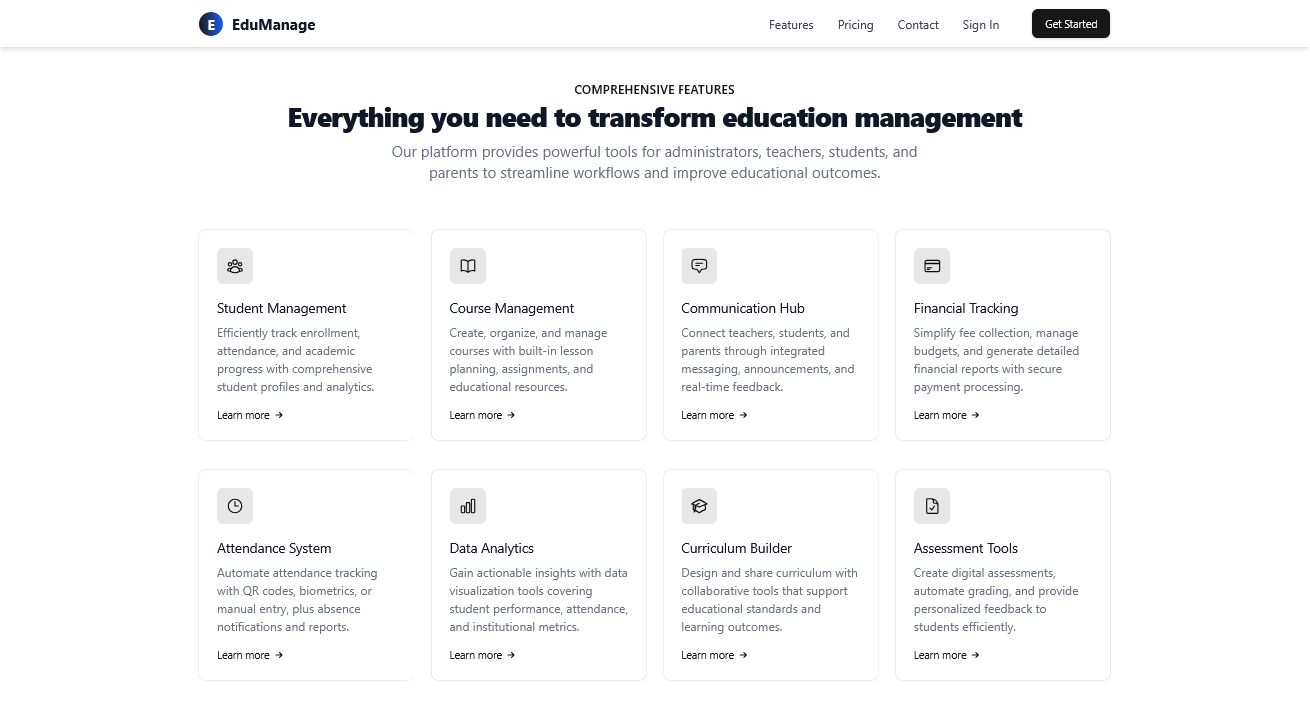
\includegraphics[width=0.85\textwidth,keepaspectratio]{pfe-pics/landing/info.png}
  \caption{\textbf{Section d'information} détaillant les caractéristiques clés de la plateforme.}
  \label{fig:landing_info}
\end{figure}

\begin{figure}[H]
  \centering
  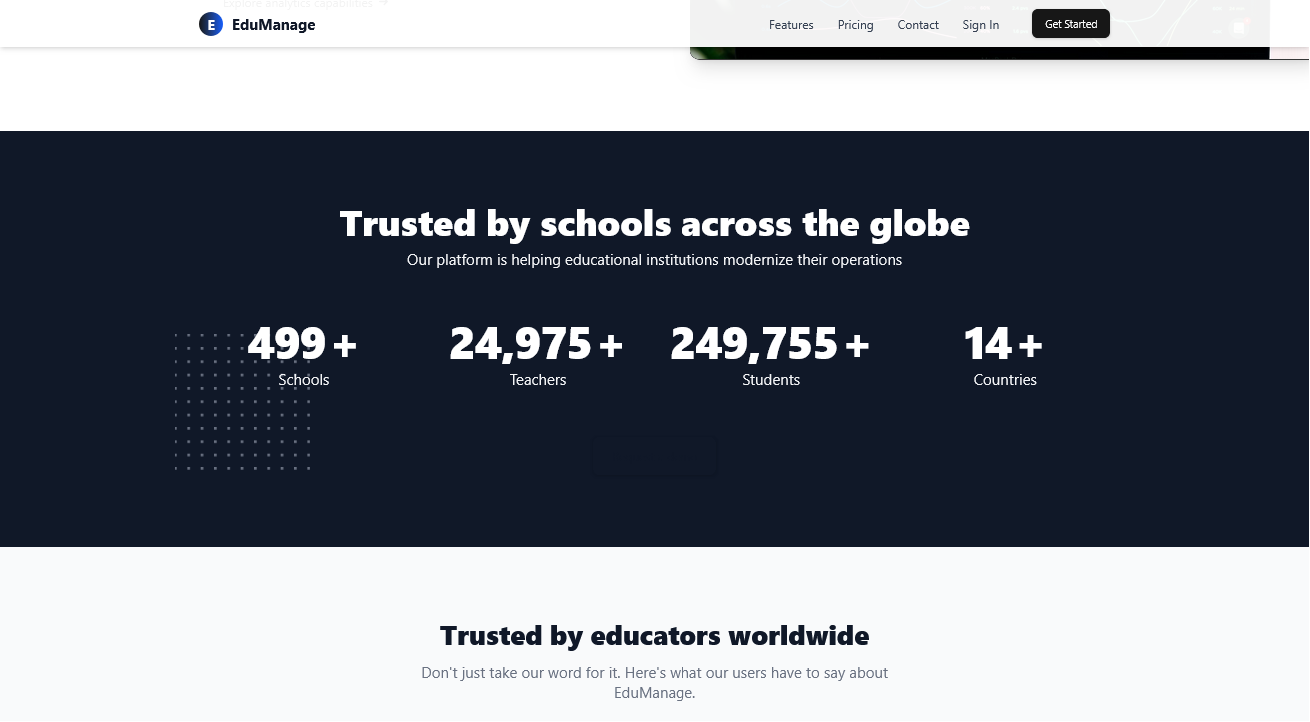
\includegraphics[width=0.85\textwidth,keepaspectratio]{pfe-pics/landing/stats.png}
  \caption{\textbf{Section de statistiques} mettant en avant les résultats et l'impact du système.}
  \label{fig:landing_stats}
\end{figure}

\begin{figure}[H]
  \centering
  
\includegraphics[width=0.85\textwidth,keepaspectratio]{pfe-pics/landing/Screenshot 2025-06-09 at 23-12-47 Vite React TS.png}
  \caption{\textbf{Section de tarification} présentant les différentes options d'abonnement.}
  \label{fig:landing_pricing}
\end{figure}

\begin{figure}[H]
  \centering
  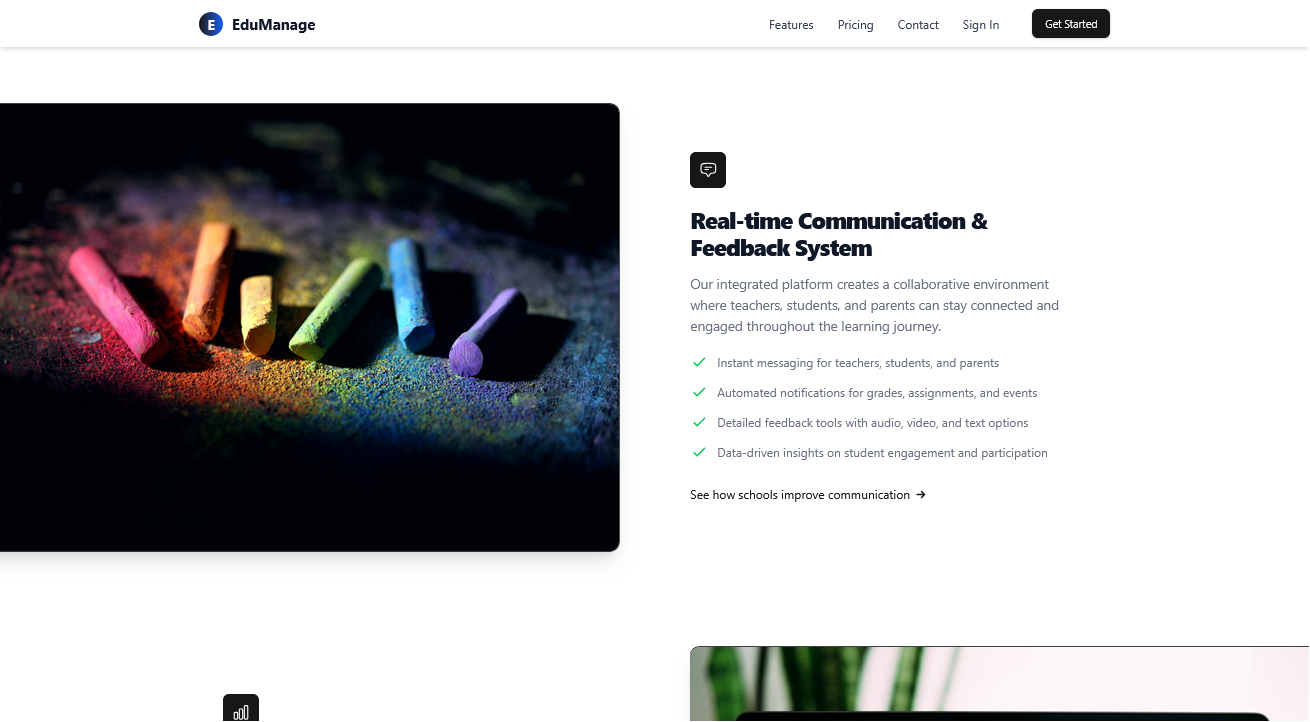
\includegraphics[width=0.85\textwidth,keepaspectratio]{pfe-pics/landing/Screenshot 2025-06-09 at 23-12-17 Vite React TS.png}
  \caption{\textbf{Section des fonctionnalités} du système de gestion scolaire.}
  \label{fig:landing_features}
\end{figure}

\begin{figure}[H]
  \centering
  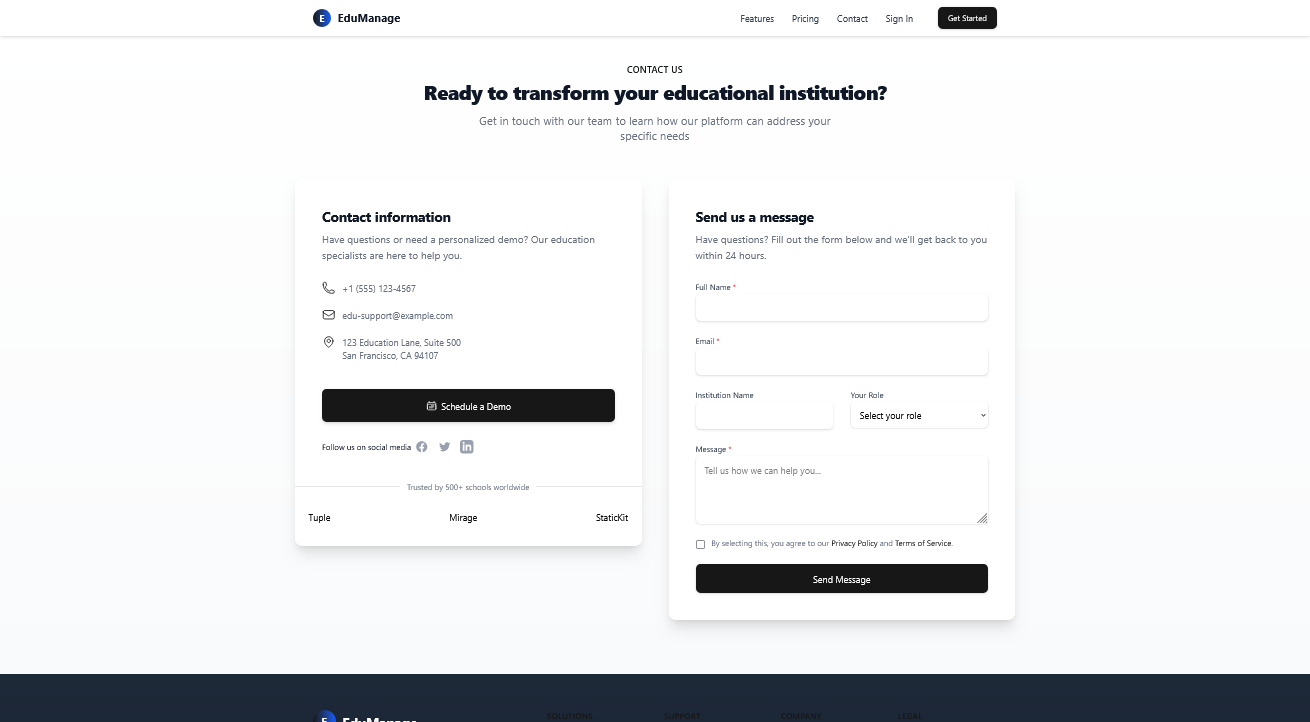
\includegraphics[width=0.85\textwidth,keepaspectratio]{pfe-pics/landing/contact.png}
  \caption{\textbf{Section de contact} avec formulaire permettant aux utilisateurs de demander des informations.}
  \label{fig:landing_contact}
\end{figure}

\begin{figure}[H]
  \centering
  
\includegraphics[width=0.85\textwidth,keepaspectratio]{pfe-pics/landing/fotter.png}
  \caption{\textbf{Pied de page (Footer)} contenant les liens importants et informations légales.}
  \label{fig:landing_footer}
\end{figure}

\subsection{Pages de présentation du système de gestion scolaire}

Les composants de la page d'accueil et de présentation du système de gestion scolaire travaillent ensemble pour offrir une expérience utilisateur cohérente et informative, guidant les visiteurs depuis la découverte initiale jusqu'à la prise de contact ou l'inscription.

\section{Environnement de développement personnel}

Pour le développement de ces deux systèmes complémentaires, un environnement de développement personnel optimisé a été configuré, permettant une productivité maximale et une expérience de développement fluide.

\subsection{Système d'exploitation et outils principaux}

\begin{itemize}
  \item \textbf{Système d'exploitation} : Arch Linux, choisi pour sa flexibilité, sa légèreté et sa capacité de personnalisation avancée
  
  \item \textbf{Éditeur de code principal} : Neovim avec une configuration personnalisée incluant des plugins pour le développement web, Python et TypeScript
  
  \item \textbf{Éditeur secondaire} : VSCodium (version open-source de VS Code), utilisé principalement pour le débogage et les fonctionnalités d'édition collaboratives
  
  \item \textbf{Terminal} : Alacritty avec configuration tmux pour la gestion efficace des sessions multiples
  
  \item \textbf{Shell} : Zsh avec le framework Oh My Zsh et des plugins pour Git, Docker et Node.js
\end{itemize}

\subsection{Environnement de base de données}

\begin{itemize}
  \item \textbf{MySQL} : Utilisé comme système de gestion de base de données relationnelle principal pour le système de gestion scolaire
  
  \item \textbf{XAMPP} : Suite de développement local intégrant Apache, MariaDB et PHP pour le développement rapide
  
  \item \textbf{PostgreSQL} : Utilisé pour le système de création de profils IA
  
  \item \textbf{MongoDB} : Utilisé pour certaines fonctionnalités spécifiques nécessitant une structure de données plus flexible
  
  \item \textbf{Redis} : Utilisé pour la mise en cache et la gestion des sessions
\end{itemize}

\subsection{Outils de développement frontend}

\begin{itemize}
  \item \textbf{Node.js} et \textbf{npm} : Pour la gestion des dépendances et l'exécution des scripts
  
  \item \textbf{Vite} : Comme outil de build rapide pour le développement frontend
  
  \item \textbf{React Developer Tools} : Pour le débogage des composants React
  
  \item \textbf{TypeScript} : Pour un développement typé et plus robuste
  
  \item \textbf{ESLint} et \textbf{Prettier} : Pour le linting et le formatage automatique du code
\end{itemize}

\subsection{Outils de développement backend}

\begin{itemize}
  \item \textbf{Postman} : Pour tester et documenter les API
  
  \item \textbf{Python avec pyenv} : Pour la gestion de plusieurs versions de Python
  
  \item \textbf{Docker} et \textbf{Docker Compose} : Pour la conteneurisation des services
  
  \item \textbf{Swagger UI} : Pour la documentation interactive des API
\end{itemize}

\section{Glossaire des abréviations}

\begin{itemize}
  \item \textbf{API} : Application Programming Interface - Interface de programmation d'application permettant la communication entre différents logiciels
  
  \item \textbf{CSS} : Cascading Style Sheets - Langage de feuille de style utilisé pour décrire la présentation d'un document écrit en HTML
  
  \item \textbf{CRUD} : Create, Read, Update, Delete - Opérations de base pour la persistance des données
  
  \item \textbf{DOM} : Document Object Model - Interface de programmation pour les documents HTML et XML
  
  \item \textbf{IA} : Intelligence Artificielle - Ensemble des théories et techniques développant des programmes informatiques complexes capables de simuler certains traits de l'intelligence humaine
  
  \item \textbf{JWT} : JSON Web Token - Standard ouvert basé sur JSON pour créer des jetons d'accès
  
  \item \textbf{LLM} : Large Language Model - Modèle de langage de grande taille utilisé pour générer et comprendre le langage naturel
  
  \item \textbf{ORM} : Object-Relational Mapping - Technique de programmation informatique qui crée une couche d'abstraction entre la base de données relationnelle et le modèle objet
  
  \item \textbf{REST} : Representational State Transfer - Style d'architecture pour les systèmes distribués
  
  \item \textbf{SSO} : Single Sign-On - Méthode permettant à un utilisateur d'accéder à plusieurs applications avec un seul identifiant
  
  \item \textbf{UI} : User Interface - Interface utilisateur, partie visible d'une application avec laquelle interagit l'utilisateur
  
  \item \textbf{UX} : User Experience - Expérience utilisateur, ensemble des interactions et expériences vécues par l'utilisateur
  
  \item \textbf{WSGI} : Web Server Gateway Interface - Spécification simple et universelle pour l'interface entre les serveurs web et les applications web pour Python
  
  \item \textbf{XAMPP} : Cross-Platform (X), Apache, MariaDB, PHP, Perl - Suite logicielle constituant un environnement de développement web
\end{itemize}
